\documentclass{article}
\usepackage[left=2cm,right=2cm,top=3cm,bottom=3cm,letterpaper]{geometry}
\usepackage[spanish]{babel}
\usepackage[utf8]{inputenc}
\usepackage{graphicx}
\usepackage{enumitem}
\usepackage{hyperref}
\usepackage{graphicx}

\title{Preprocesamiento de los datos}
\author{Juan Carlos López López \and Adolfo Marín Arriaga \and Luis Rodrigo Rojo Morales}
\date{\today\\}

\begin{document}
 \maketitle
 \section{Graficación de Atributos}
 \subsection{Individualmente}
 \begin{center}
   \hbox{\hspace{-5.8em}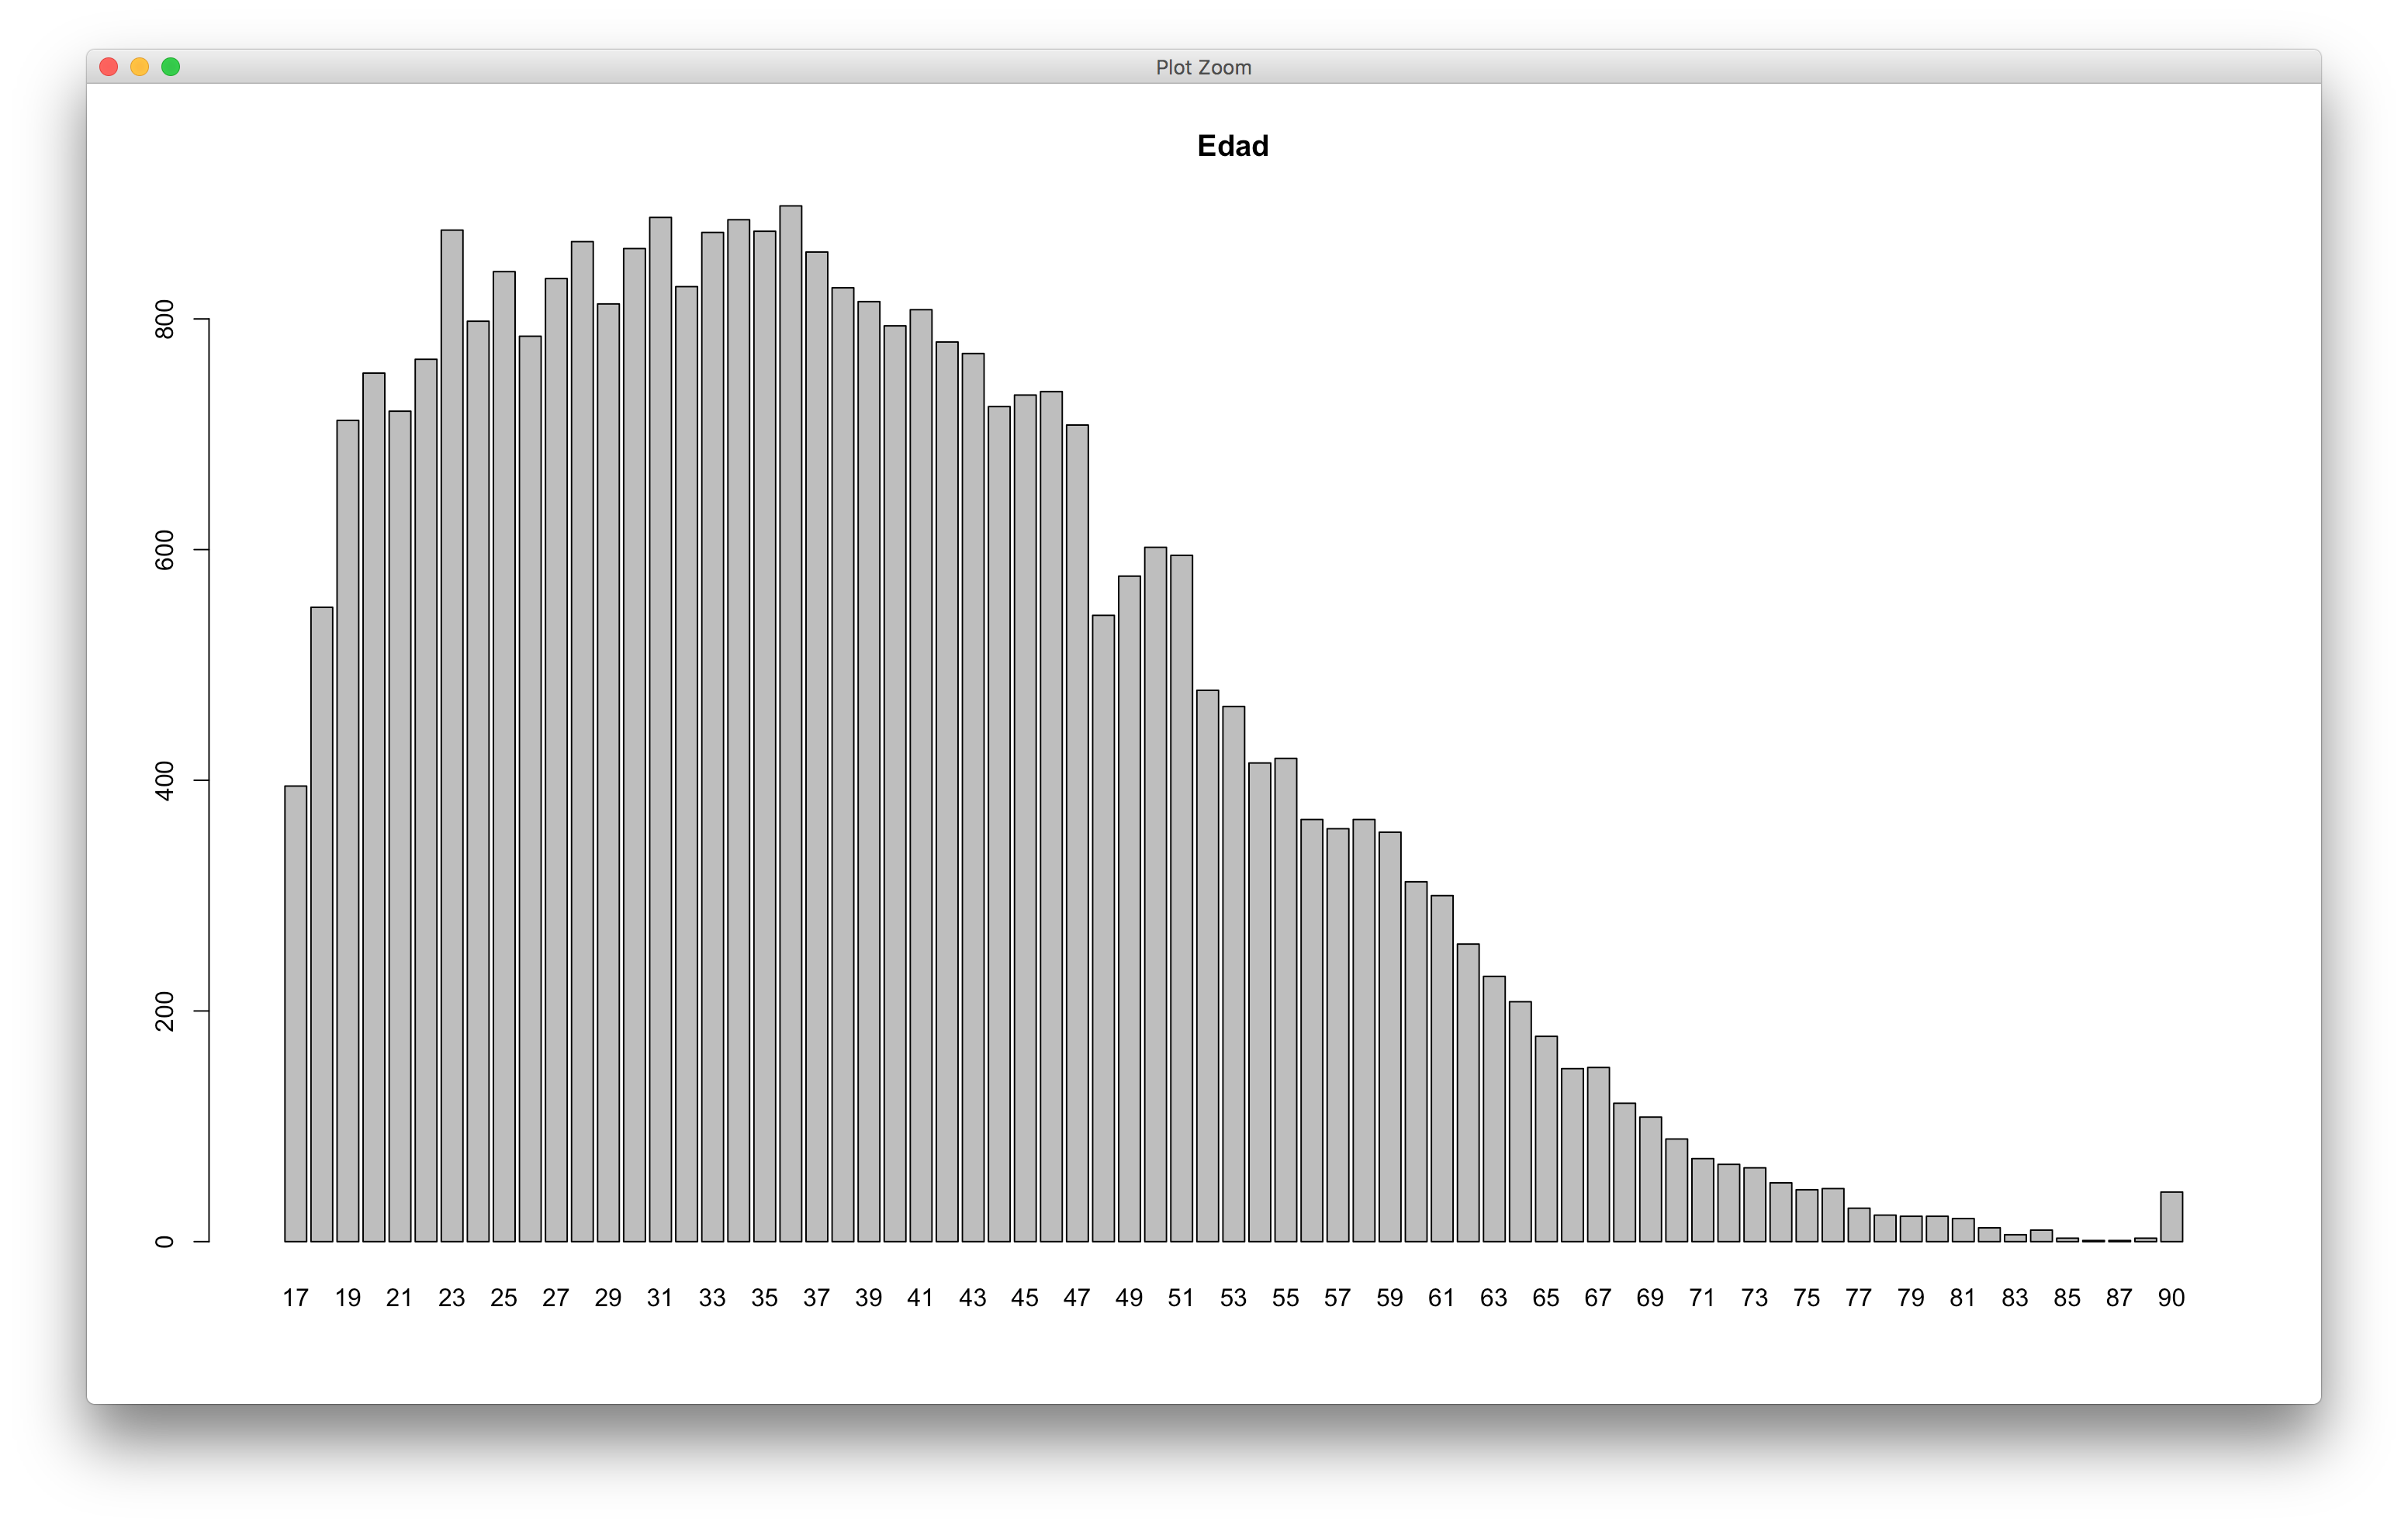
\includegraphics[scale=0.4]{graficas/edad}}
 \end{center}
 Con este atributo tomamos rangos de 10\%, los cuales quedaron de la siguiente manera: 17-21y, 22-25y, 26-29y, 30-33y, 34-37y, 38-41y, 42-45y, 46-50y, 51-57y, 58-88y
 \begin{center}
   \hbox{\hspace{-5.8em}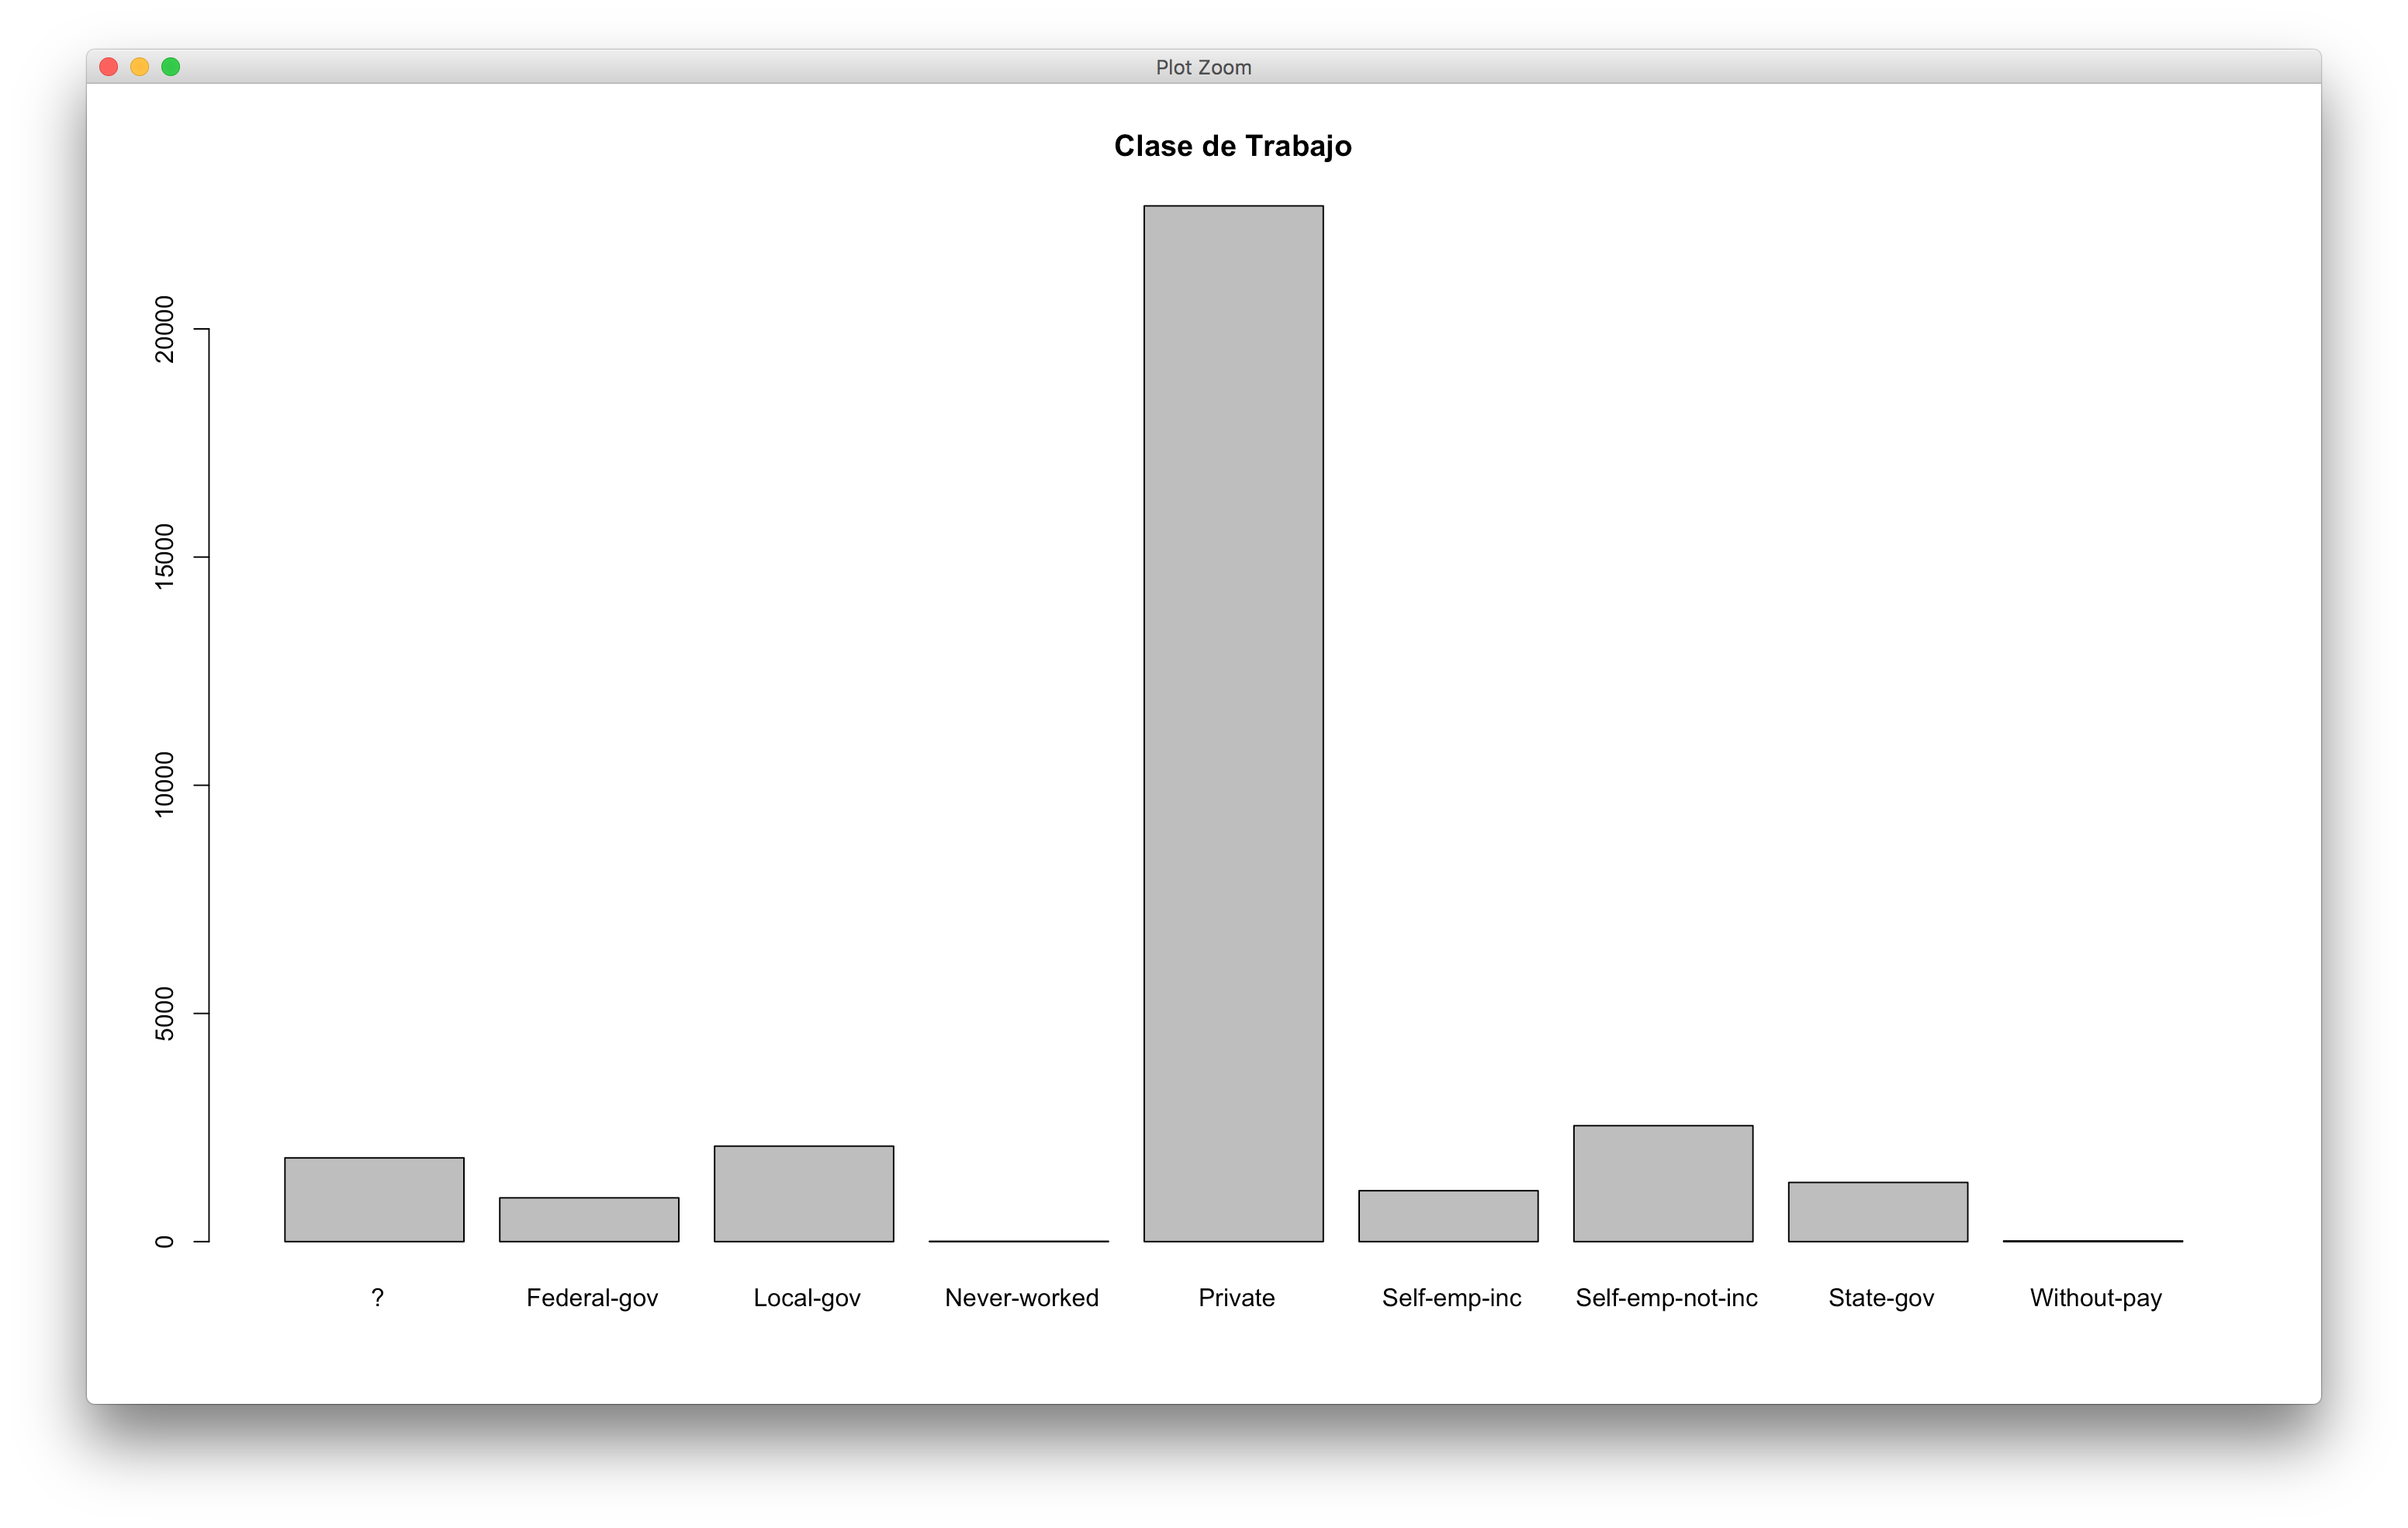
\includegraphics[scale=0.4]{graficas/claseDeTrabajo}}
 \end{center}
 \begin{center}
   \hbox{\hspace{-5.8em}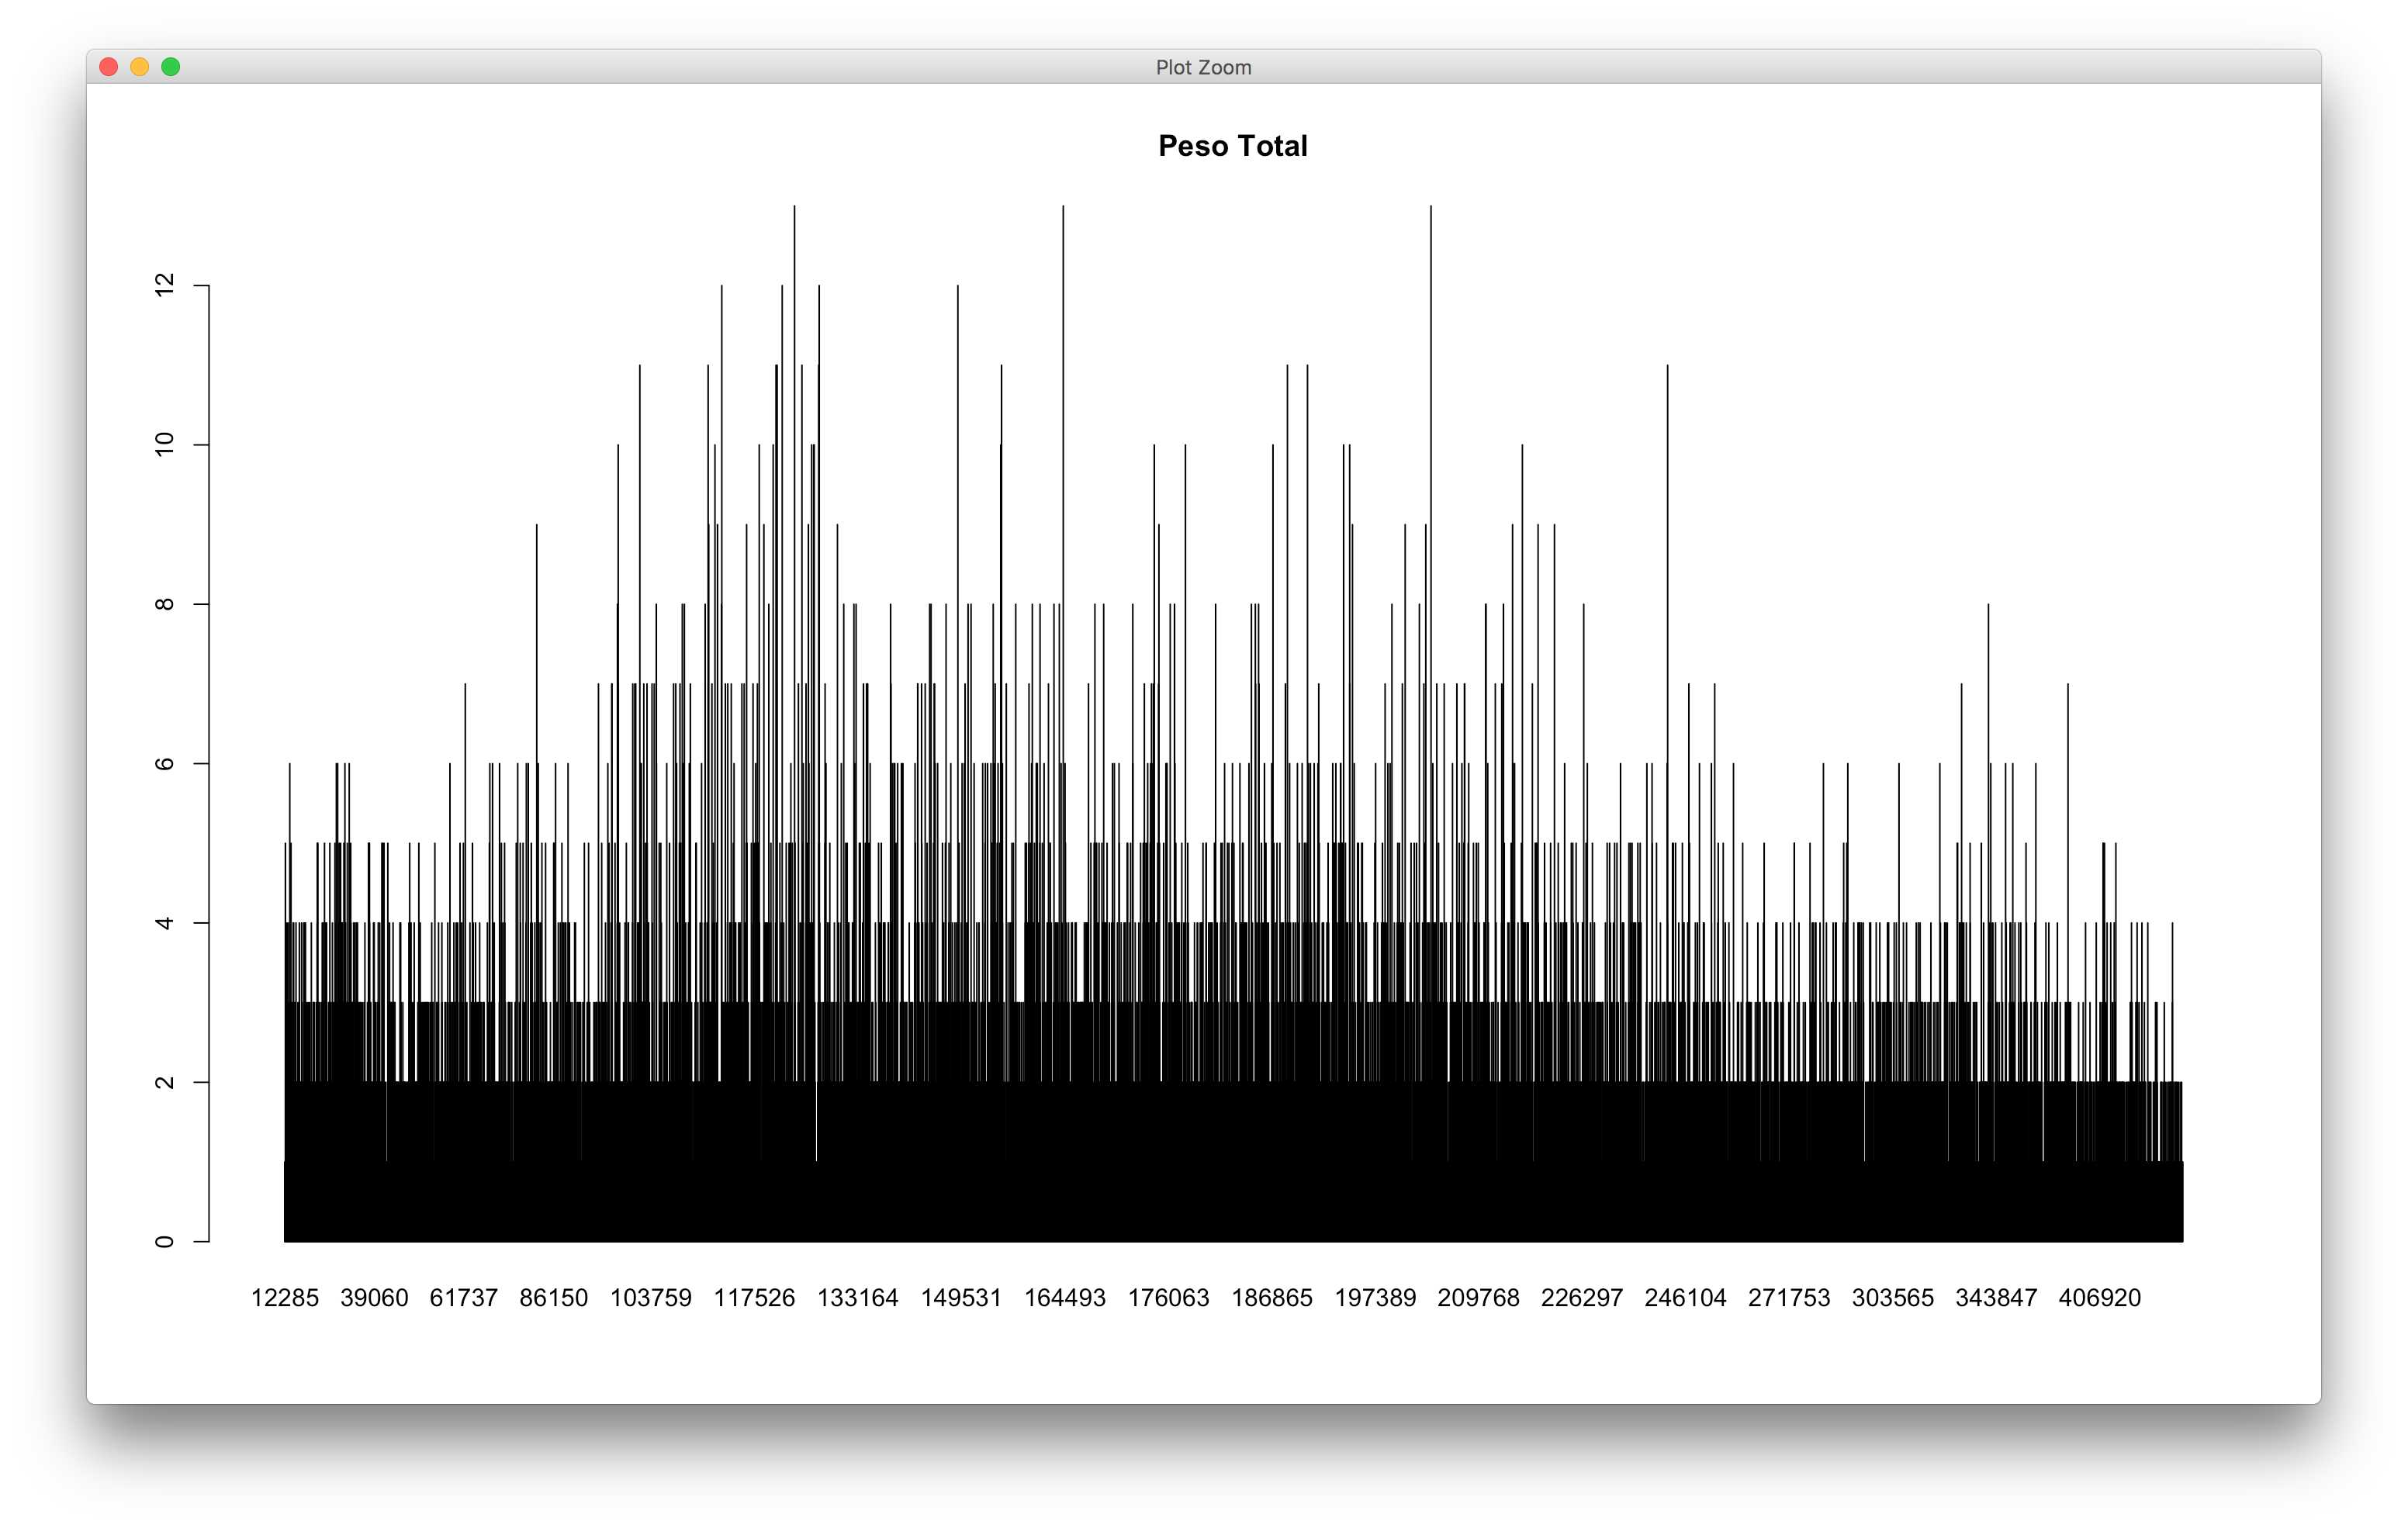
\includegraphics[scale=0.4]{graficas/pesoTotal}}
 \end{center}
 \begin{center}
   \hbox{\hspace{-5.8em}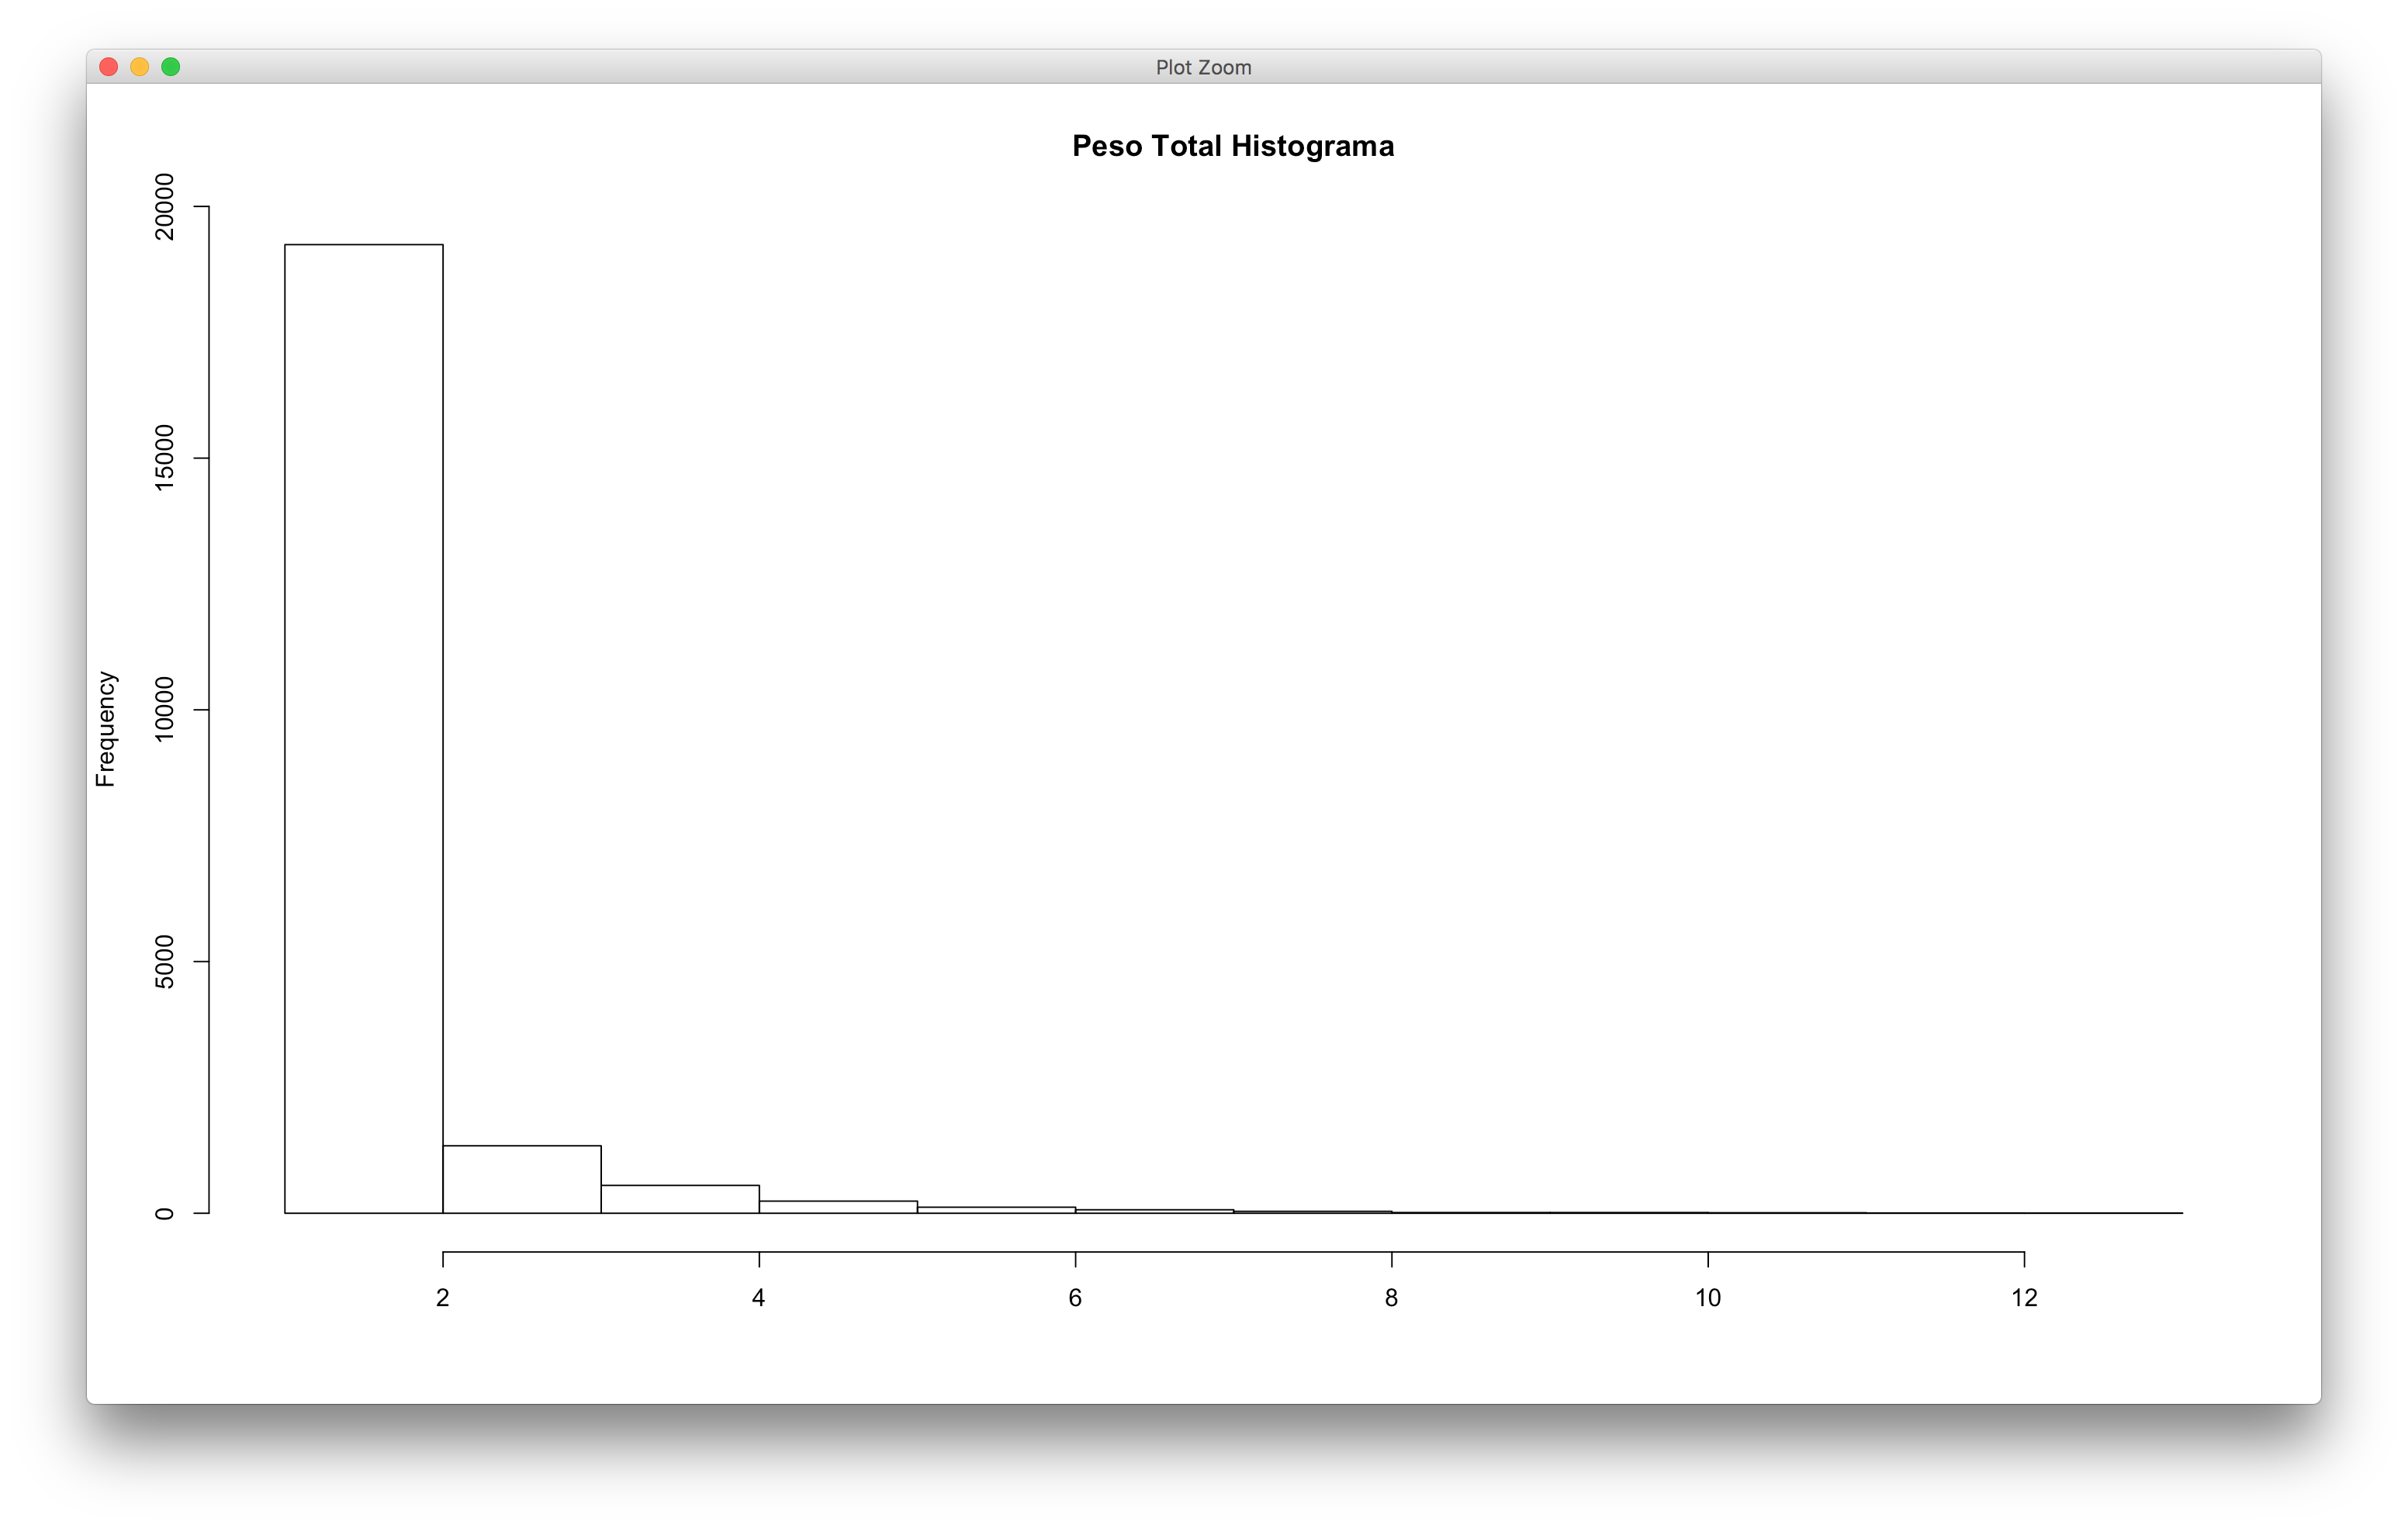
\includegraphics[scale=0.4]{graficas/pesoTotalHist}}
 \end{center}
 \begin{center}
   \hbox{\hspace{-6.1em}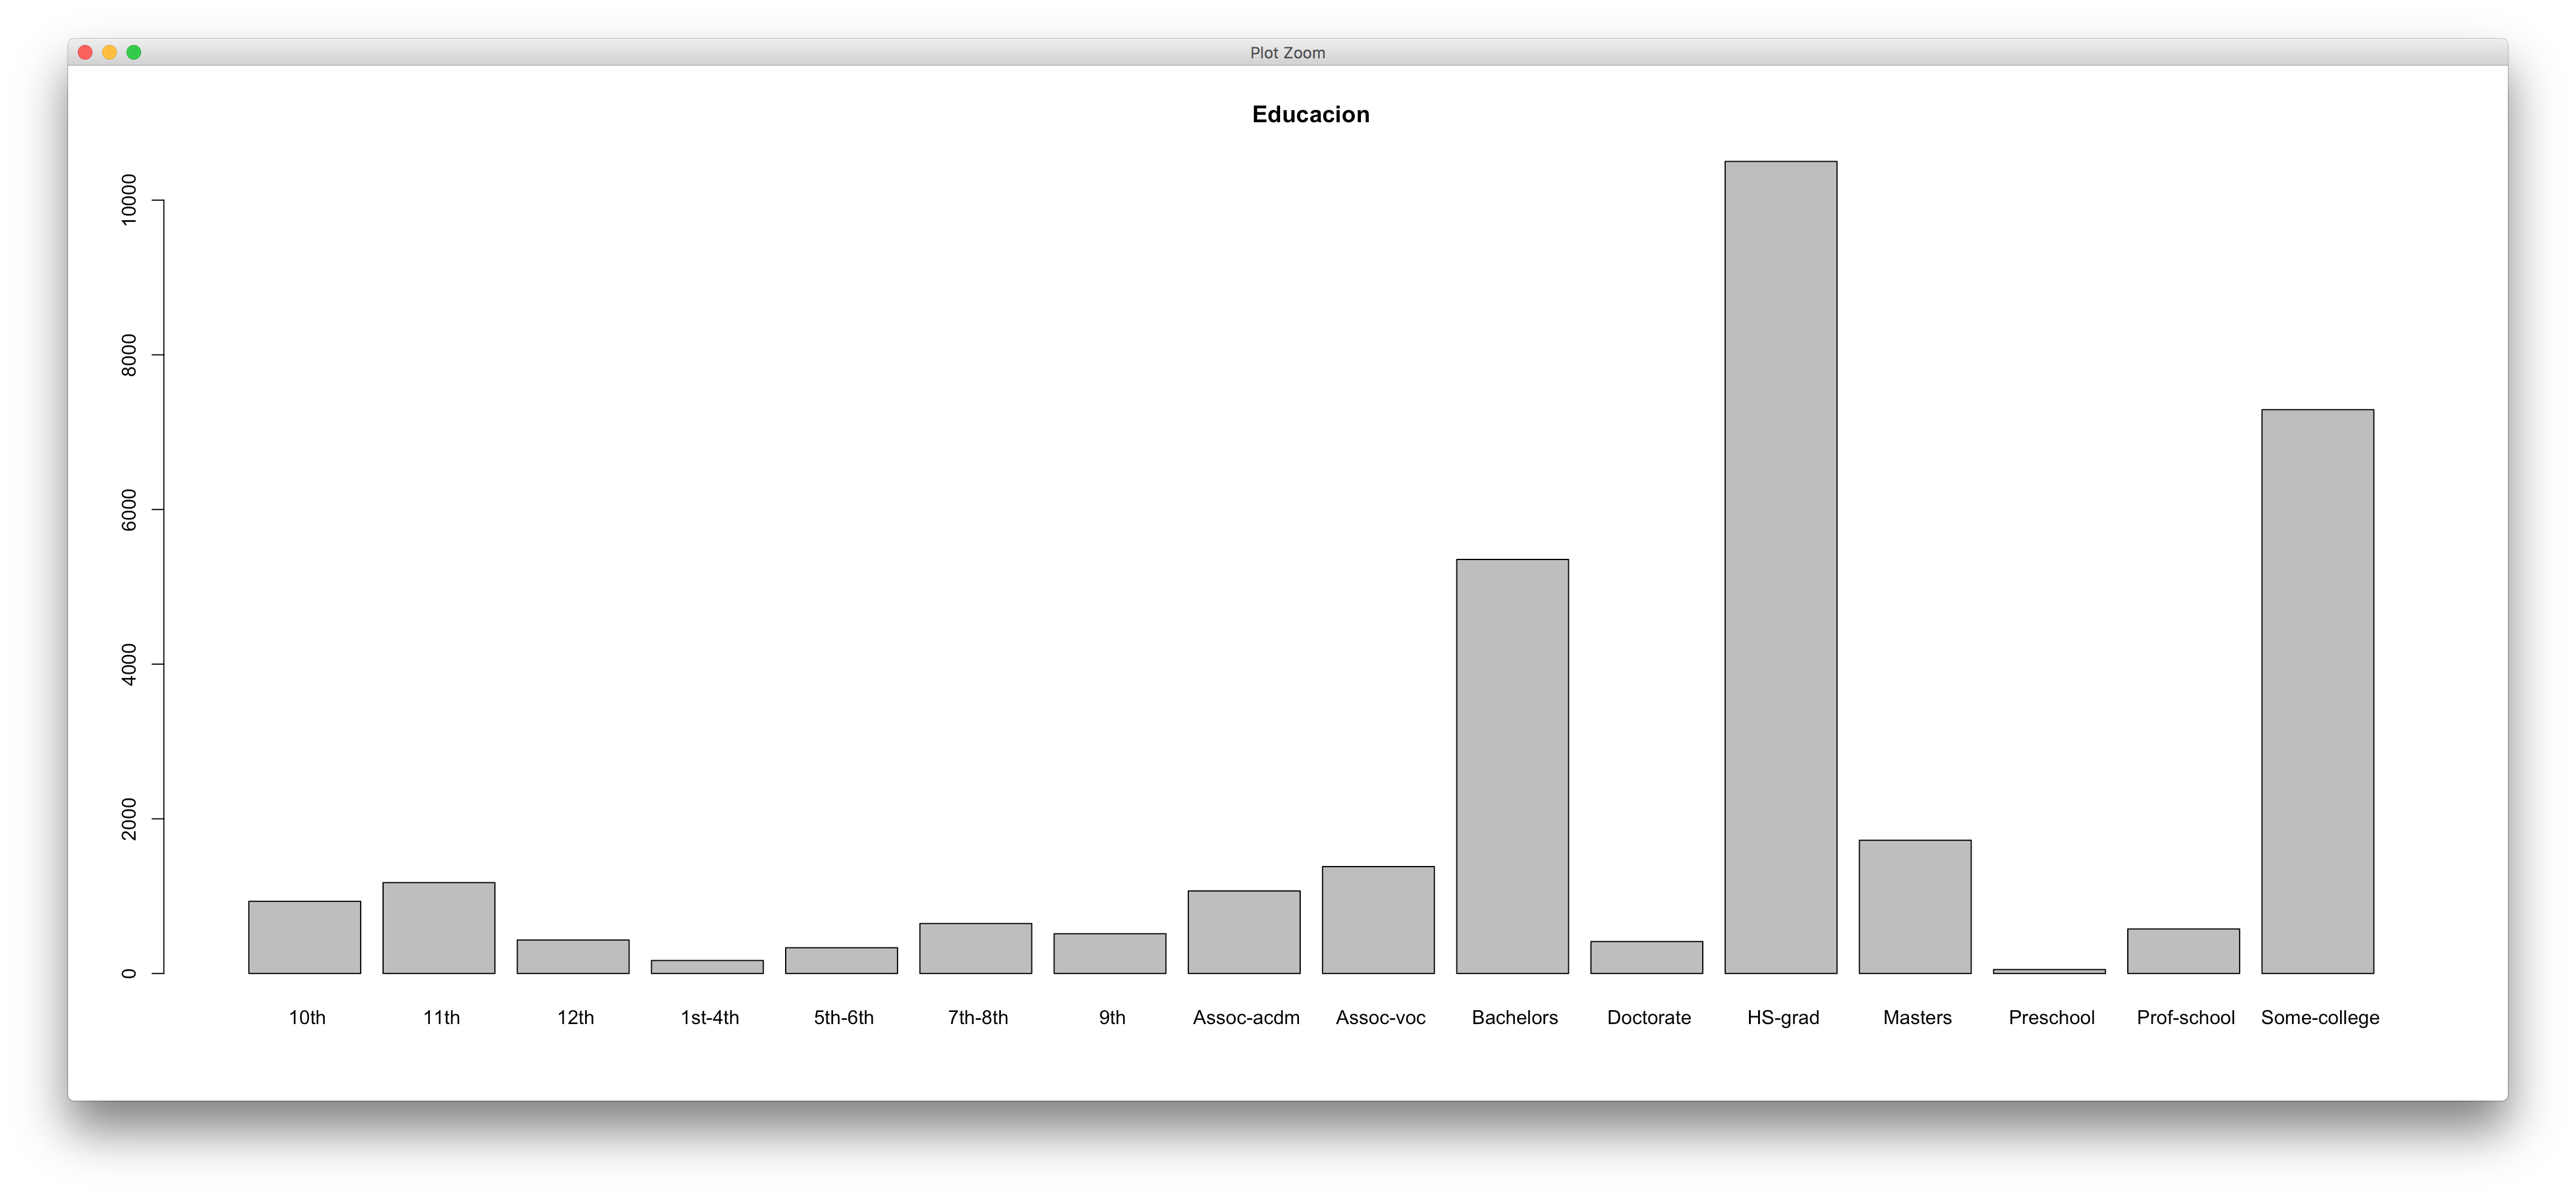
\includegraphics[scale=0.3]{graficas/educacion}}
 \end{center}
 \begin{center}
   \hbox{\hspace{-5.8em}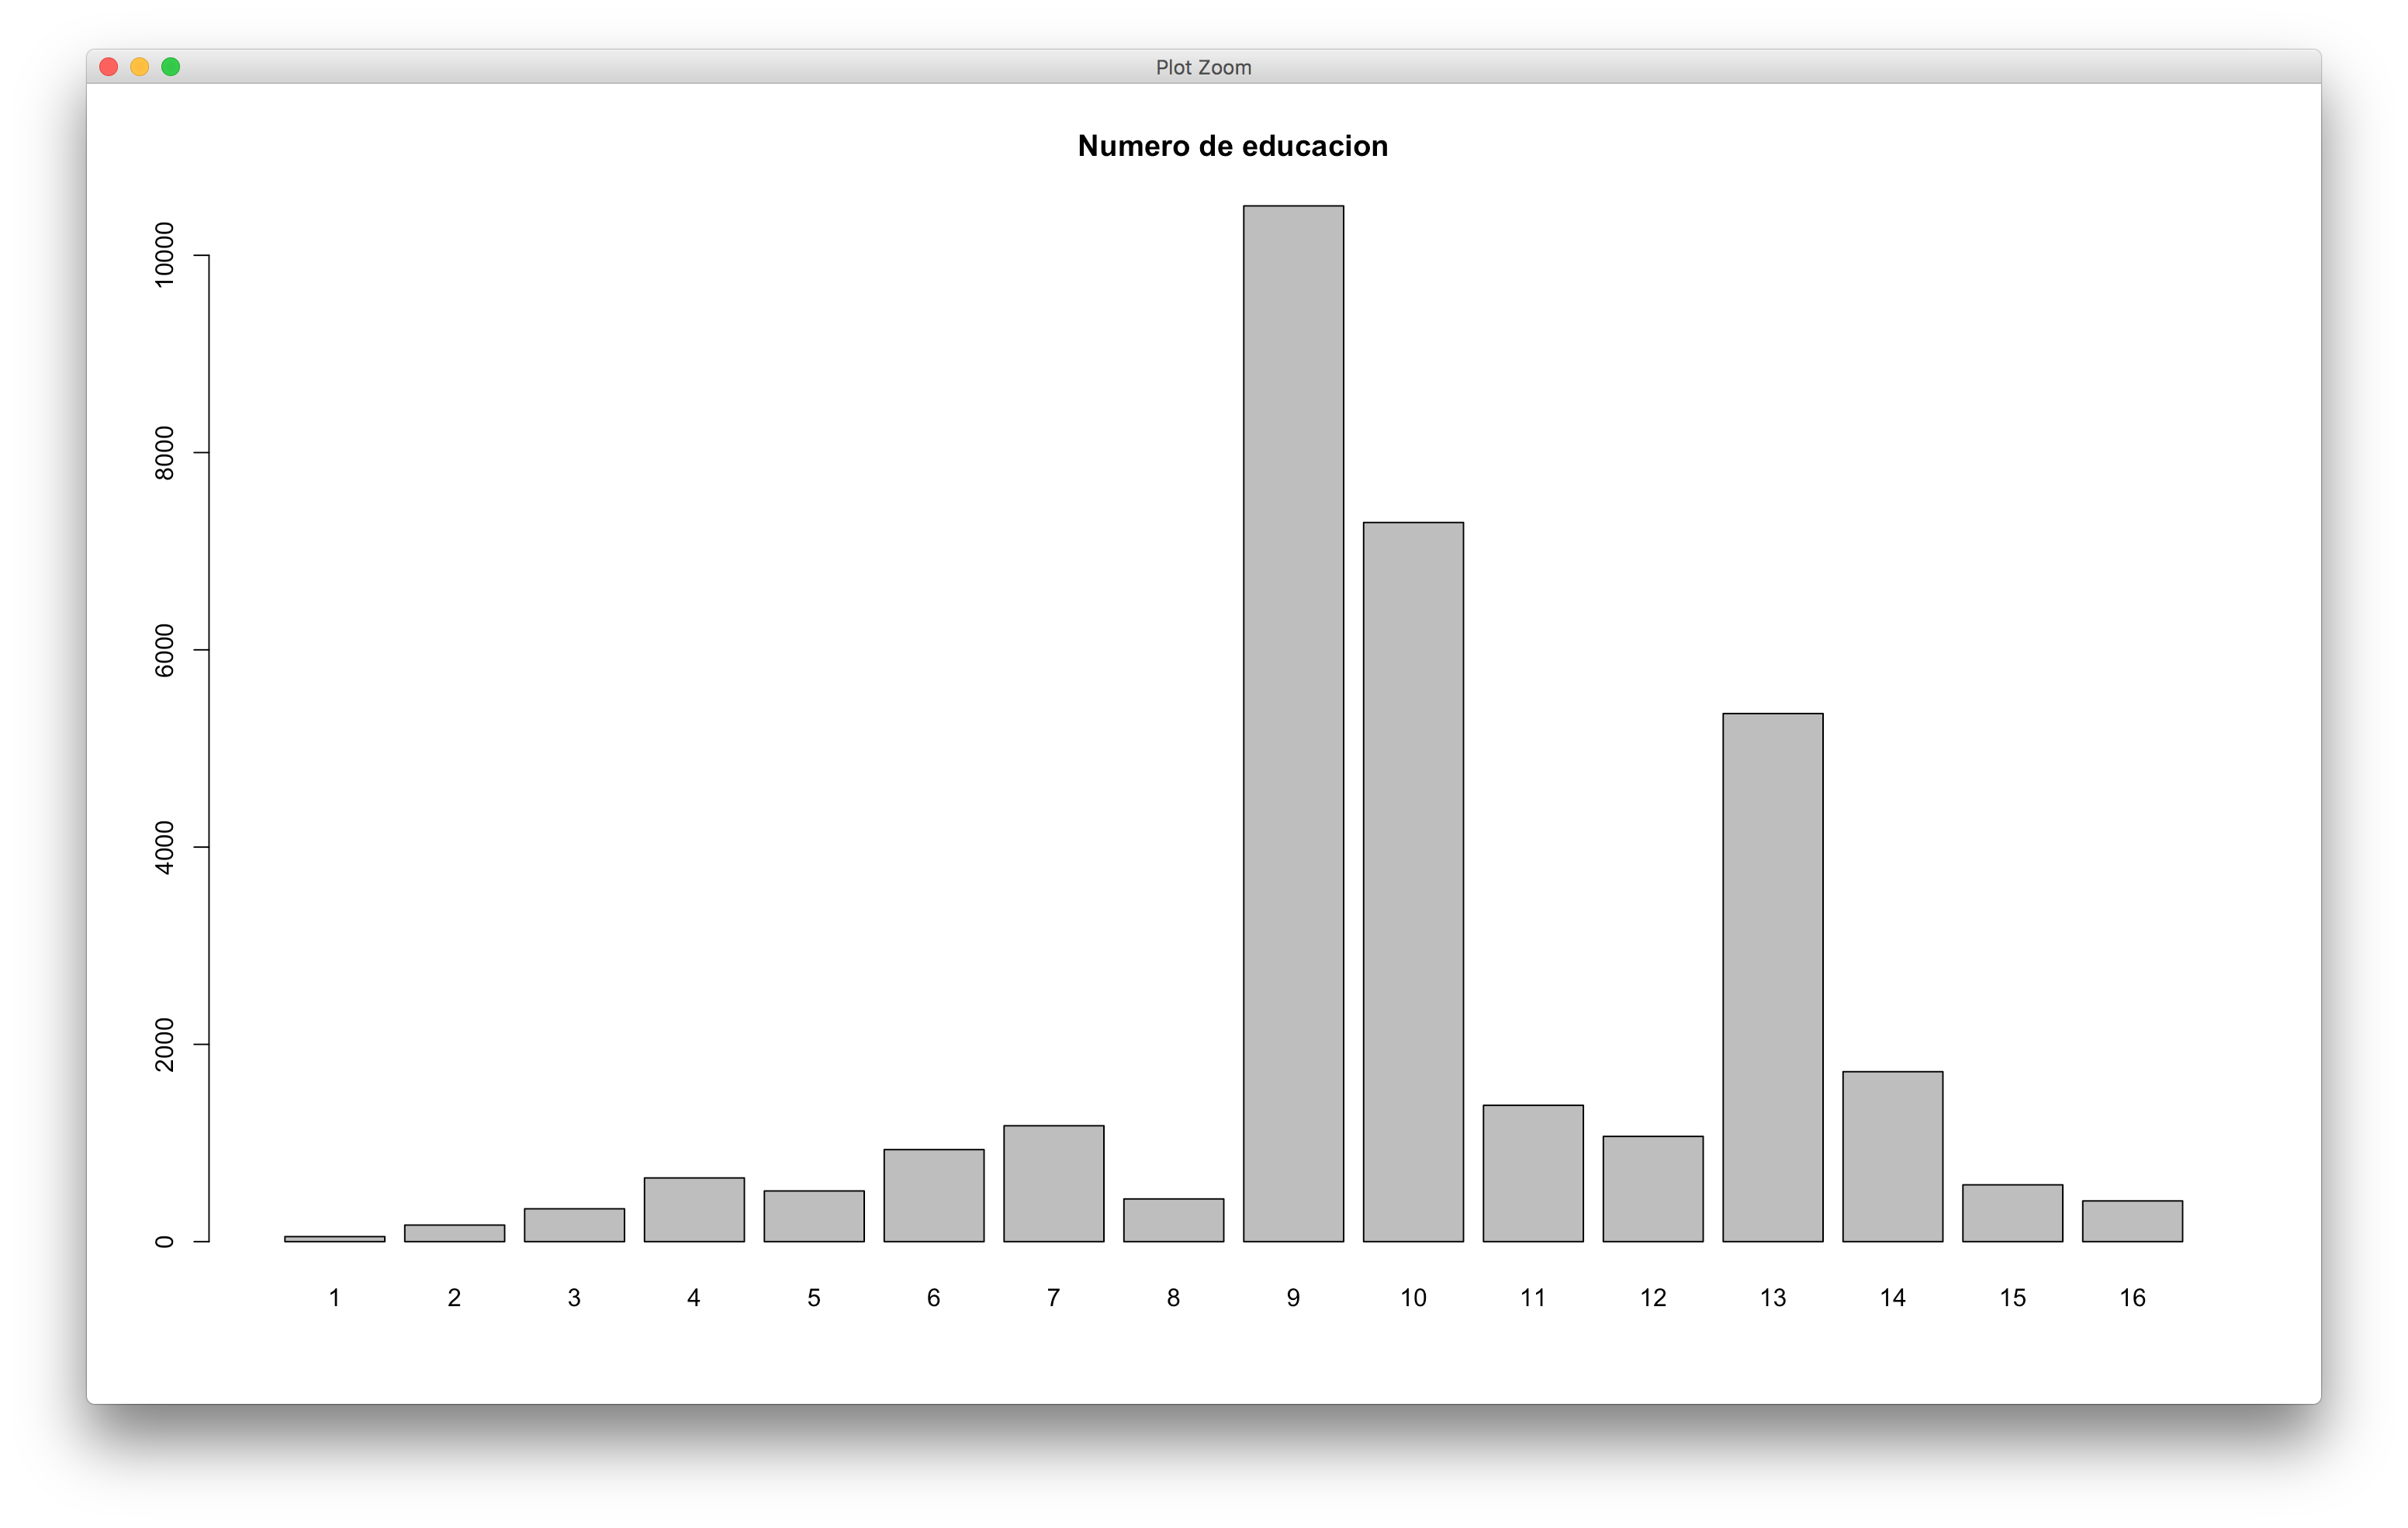
\includegraphics[scale=0.4]{graficas/numeroDeEducacion}}
 \end{center}
 \begin{center}
   \hbox{\hspace{-5.8em}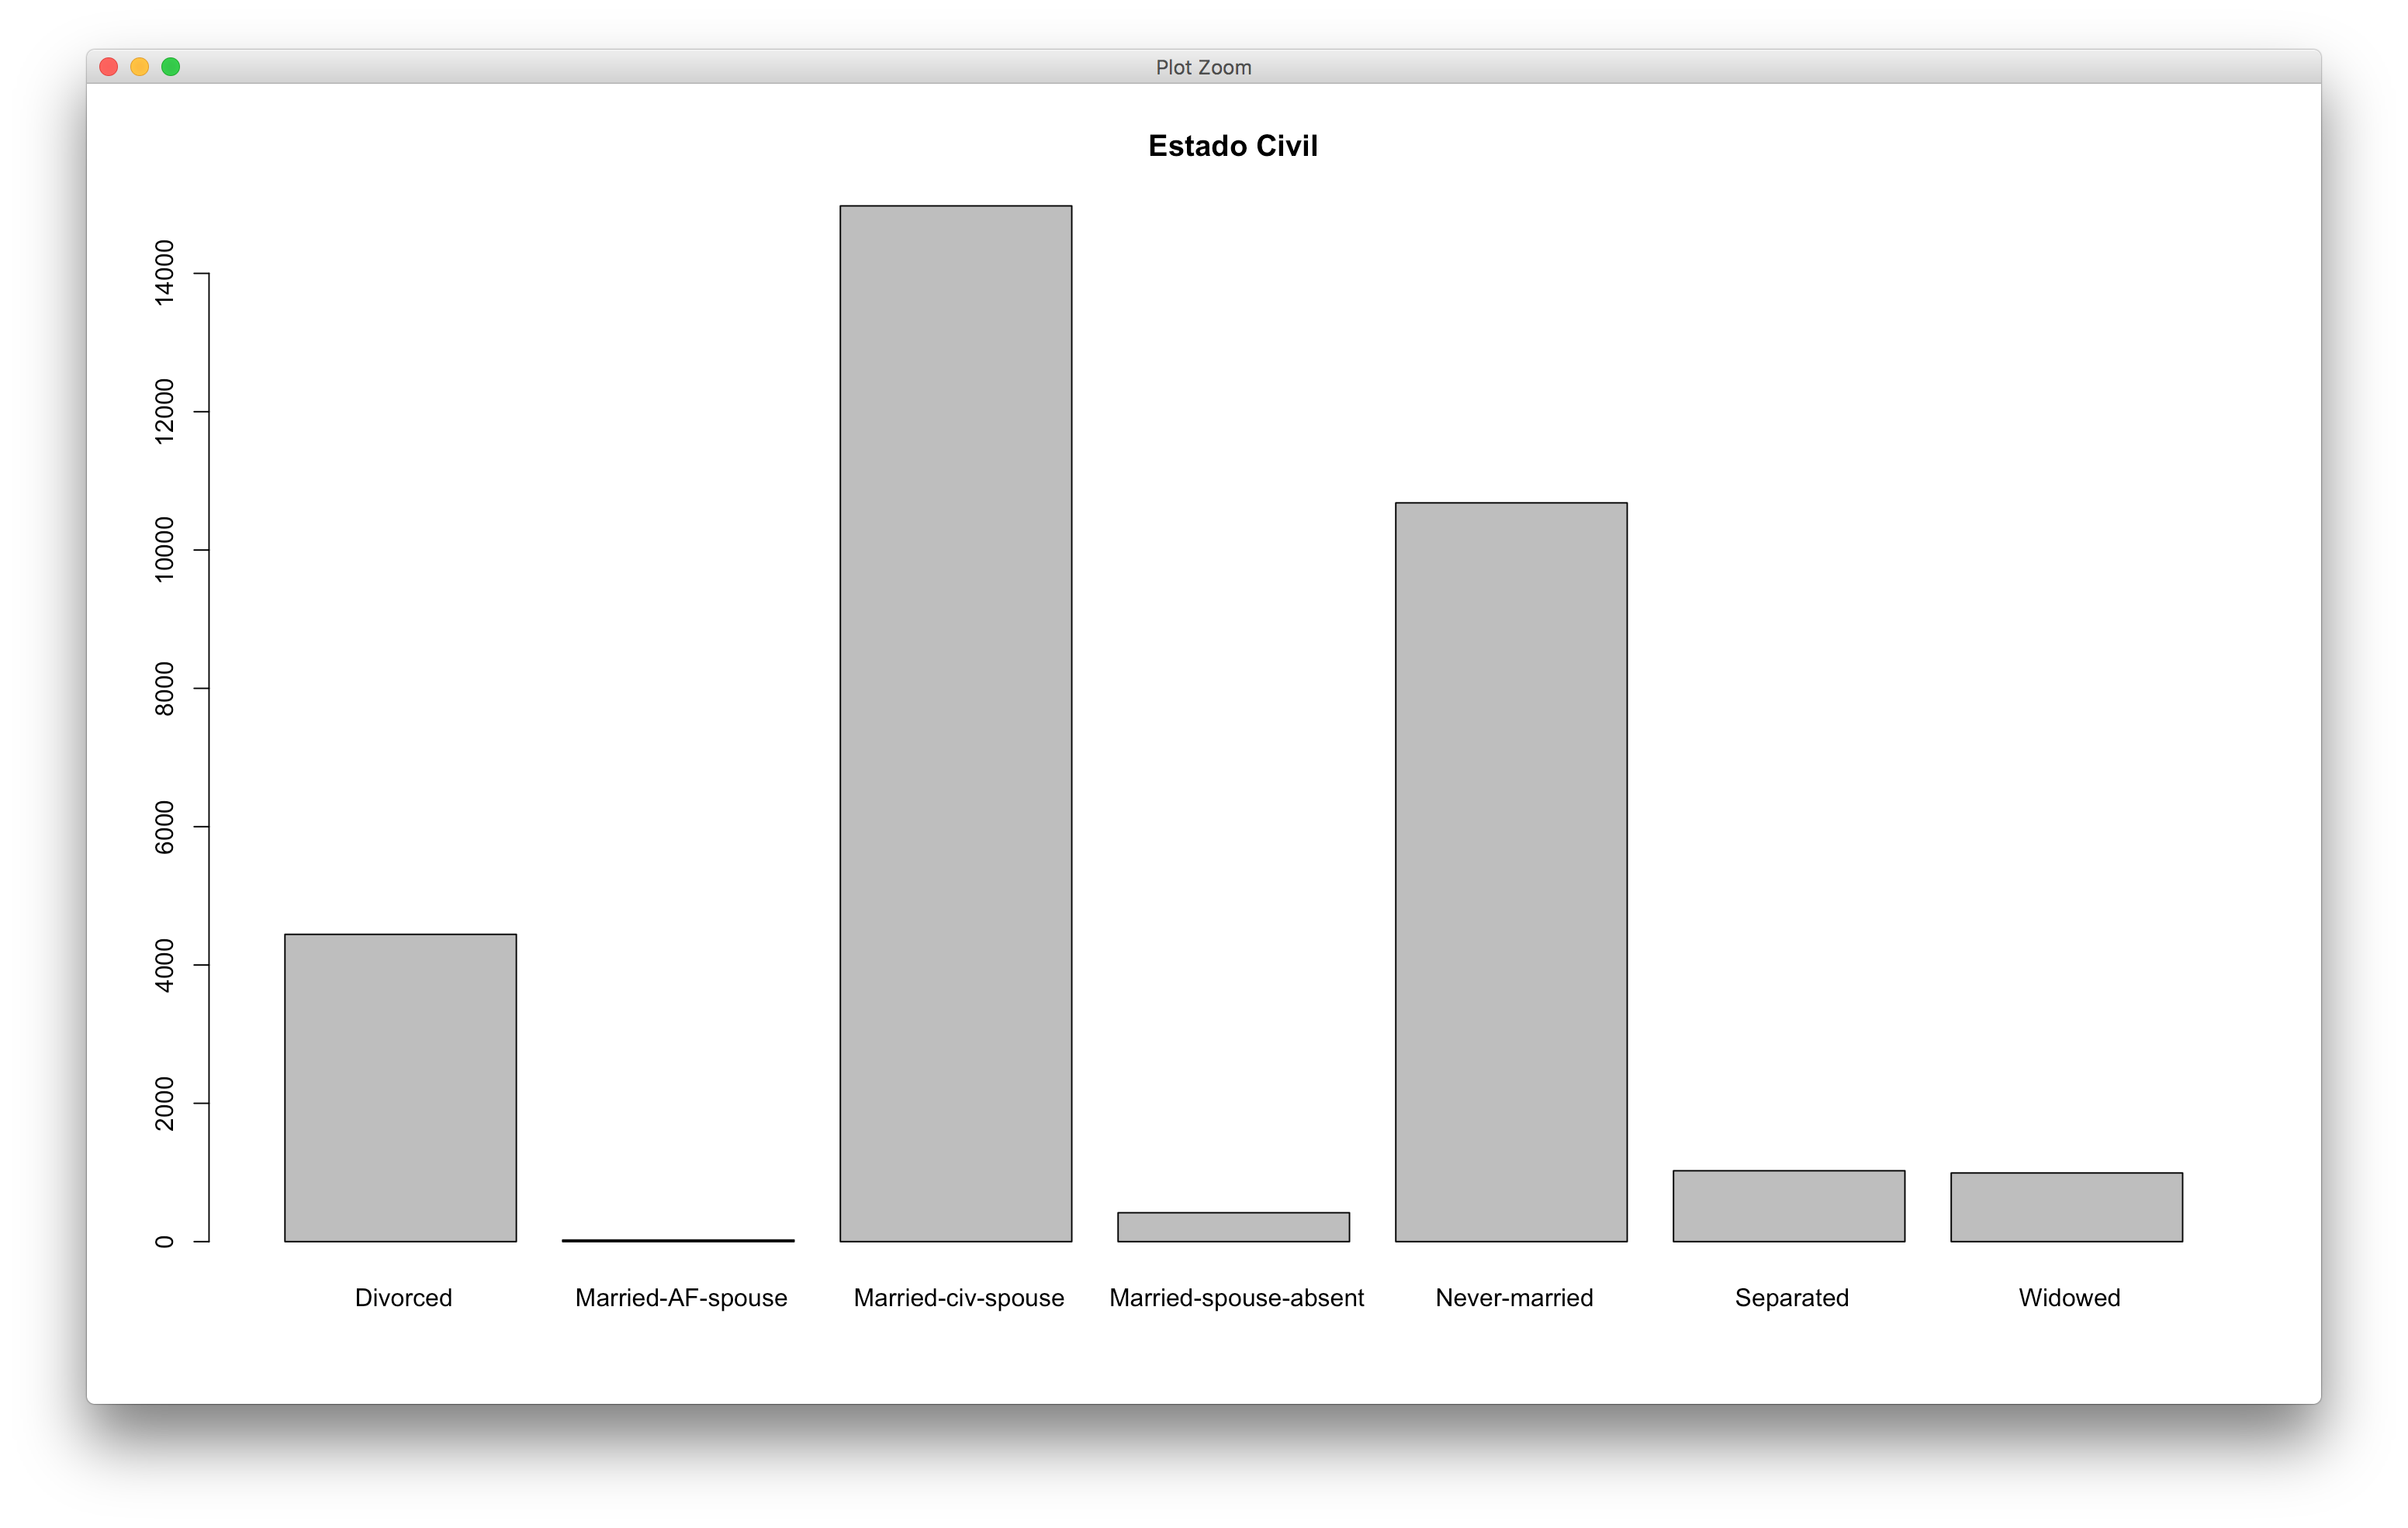
\includegraphics[scale=0.4]{graficas/EstadoCivil}}
 \end{center}
 \begin{center}
   \hbox{\hspace{-5.8em}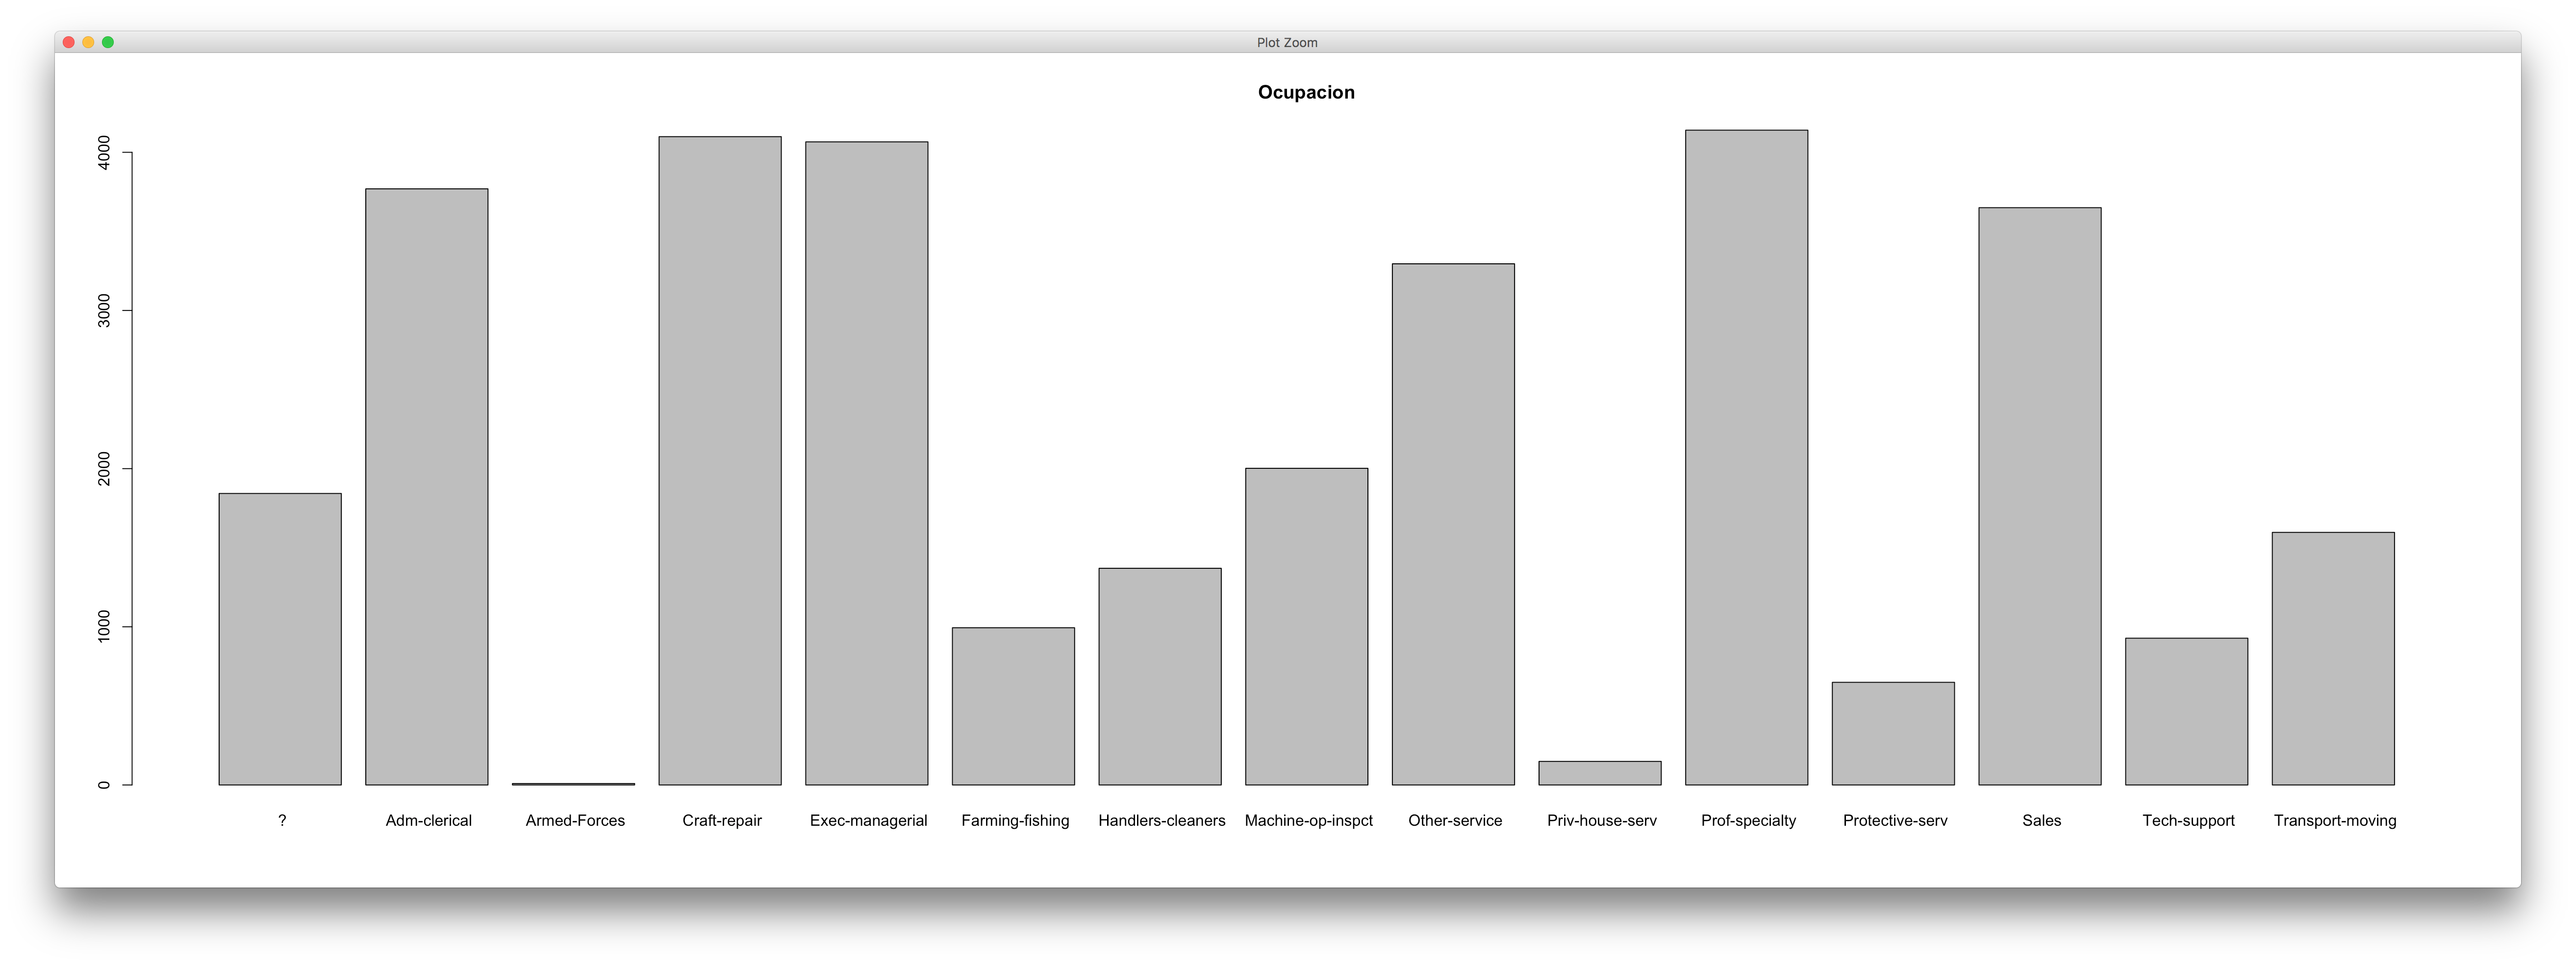
\includegraphics[scale=0.23]{graficas/ocupacion}}
 \end{center}
 \begin{center}
   \hbox{\hspace{-5.8em}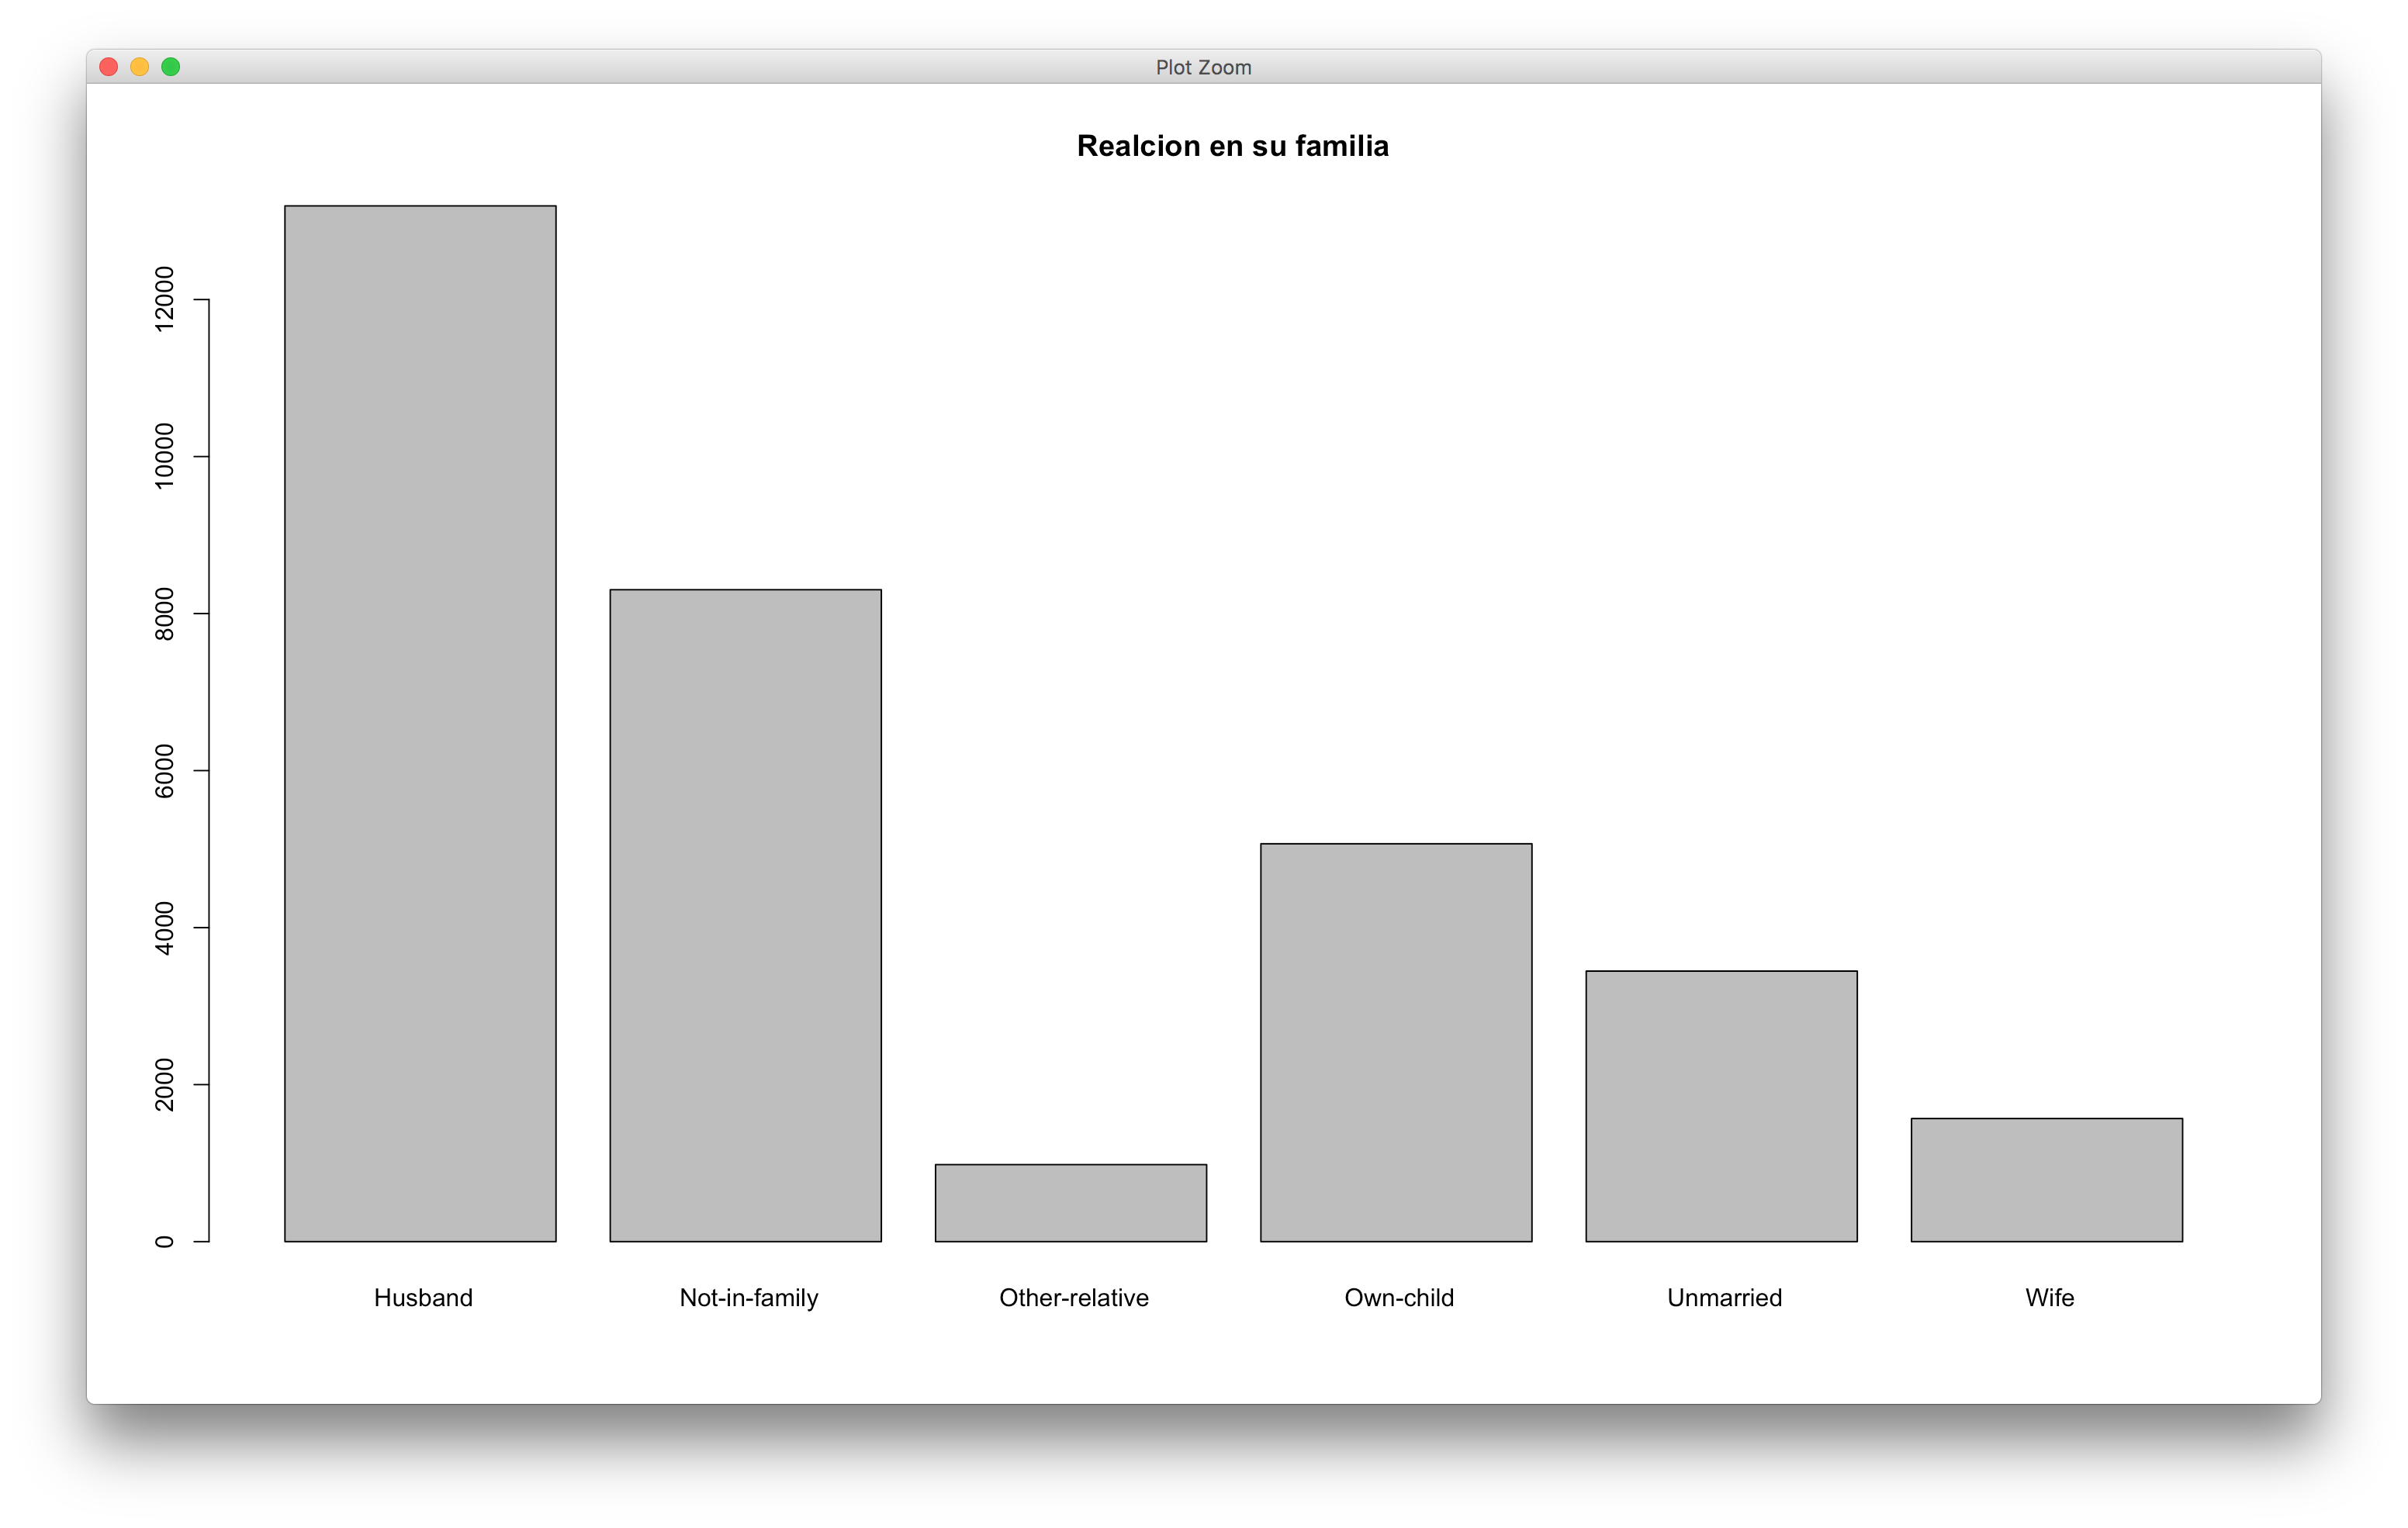
\includegraphics[scale=0.4]{graficas/relacionEnSuFamilia}}
 \end{center}
 \begin{center}
   \hbox{\hspace{-5.8em}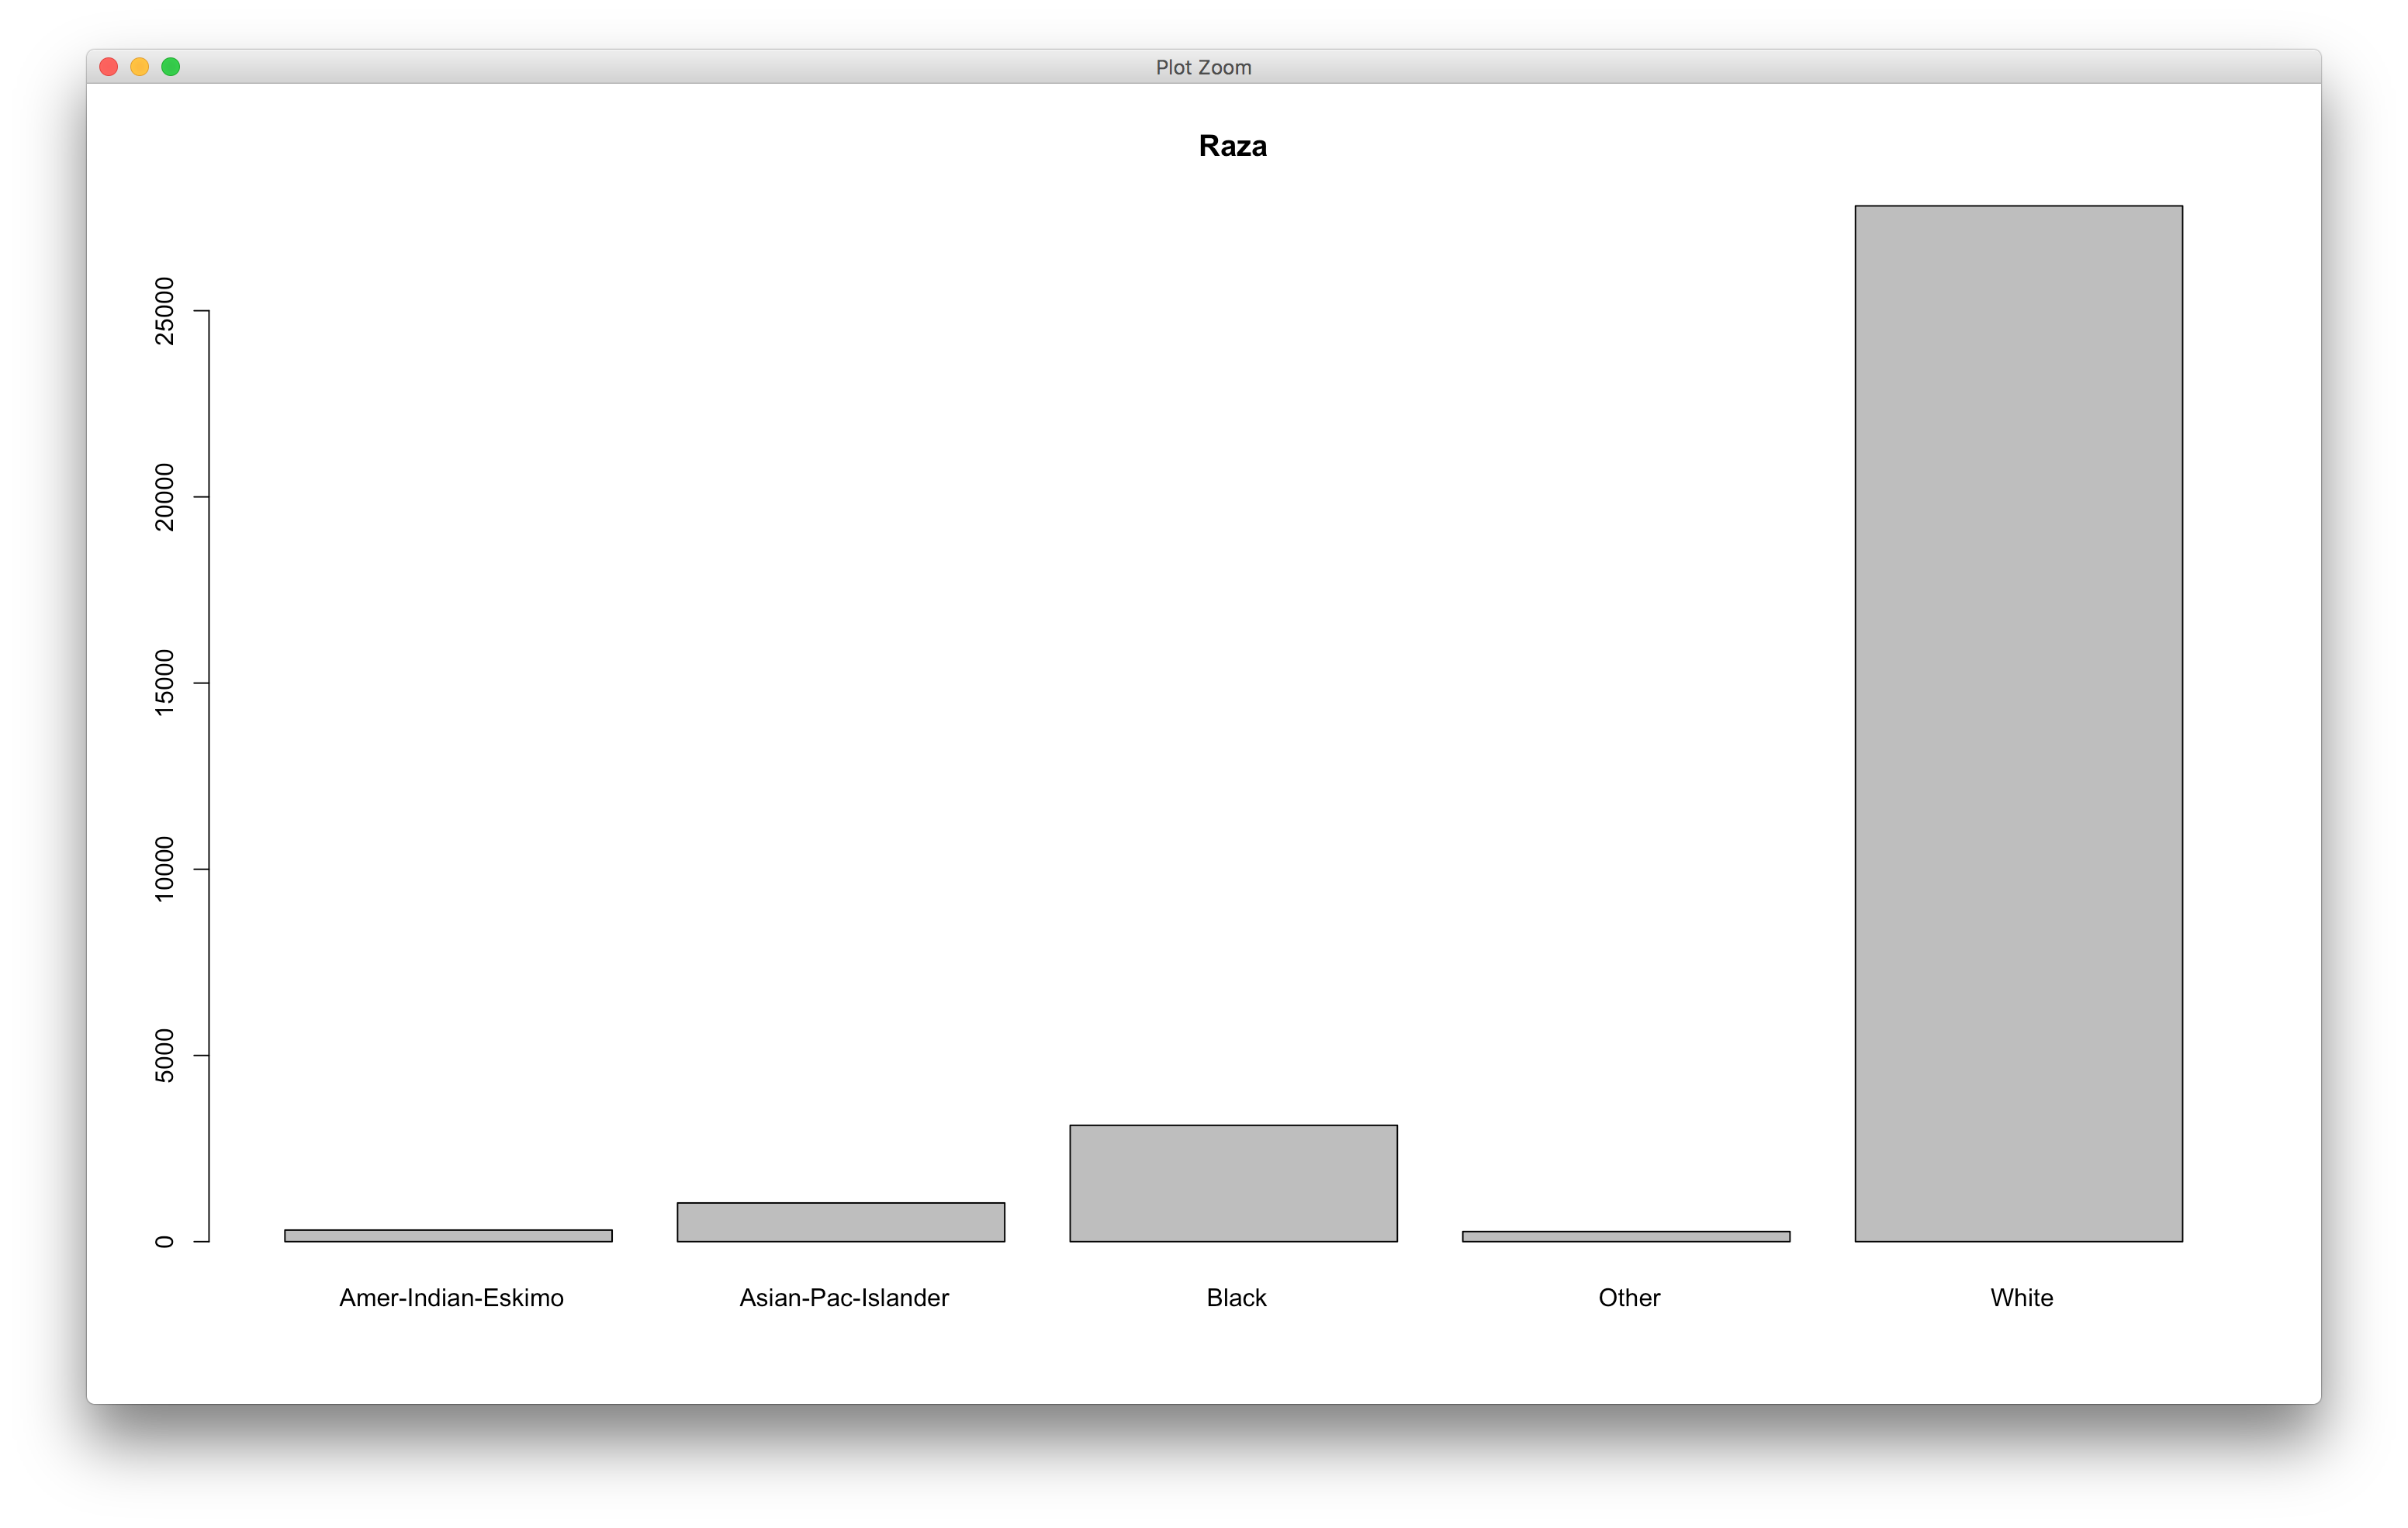
\includegraphics[scale=0.4]{graficas/raza}}
 \end{center}
 \begin{center}
   \hbox{\hspace{-5.8em}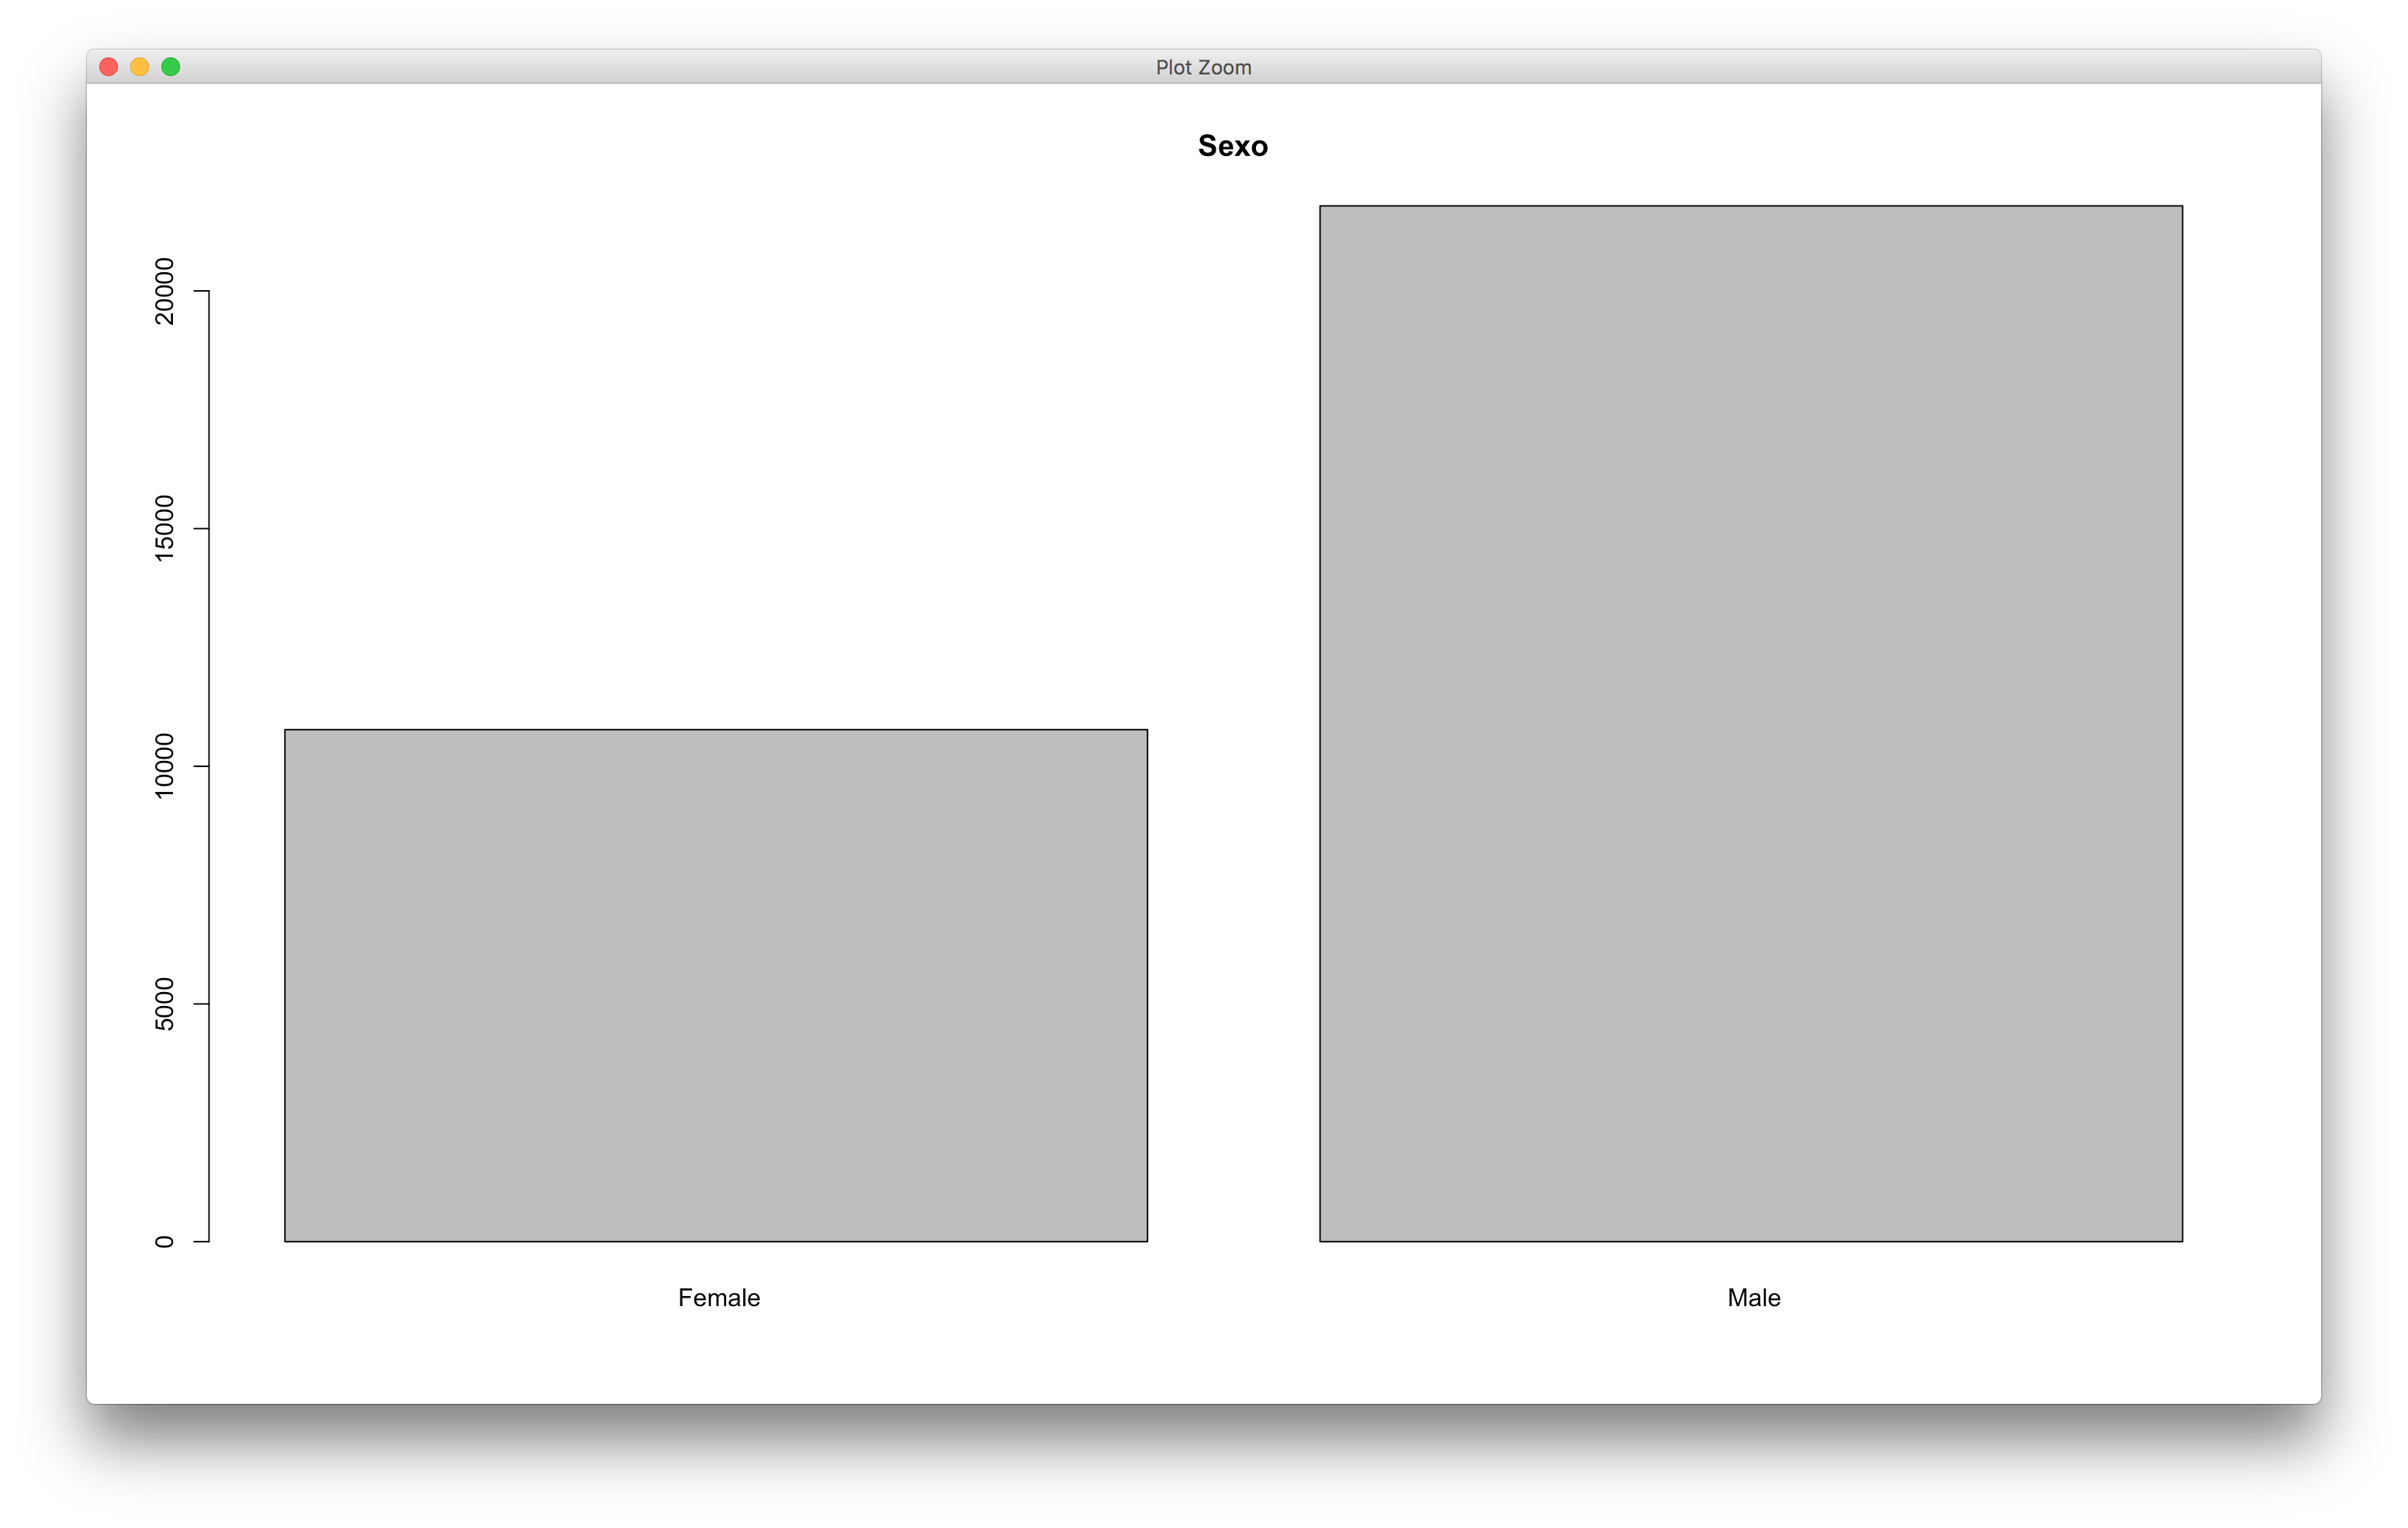
\includegraphics[scale=0.4]{graficas/sexo}}
 \end{center}
 \begin{center}
   \hbox{\hspace{-5.8em}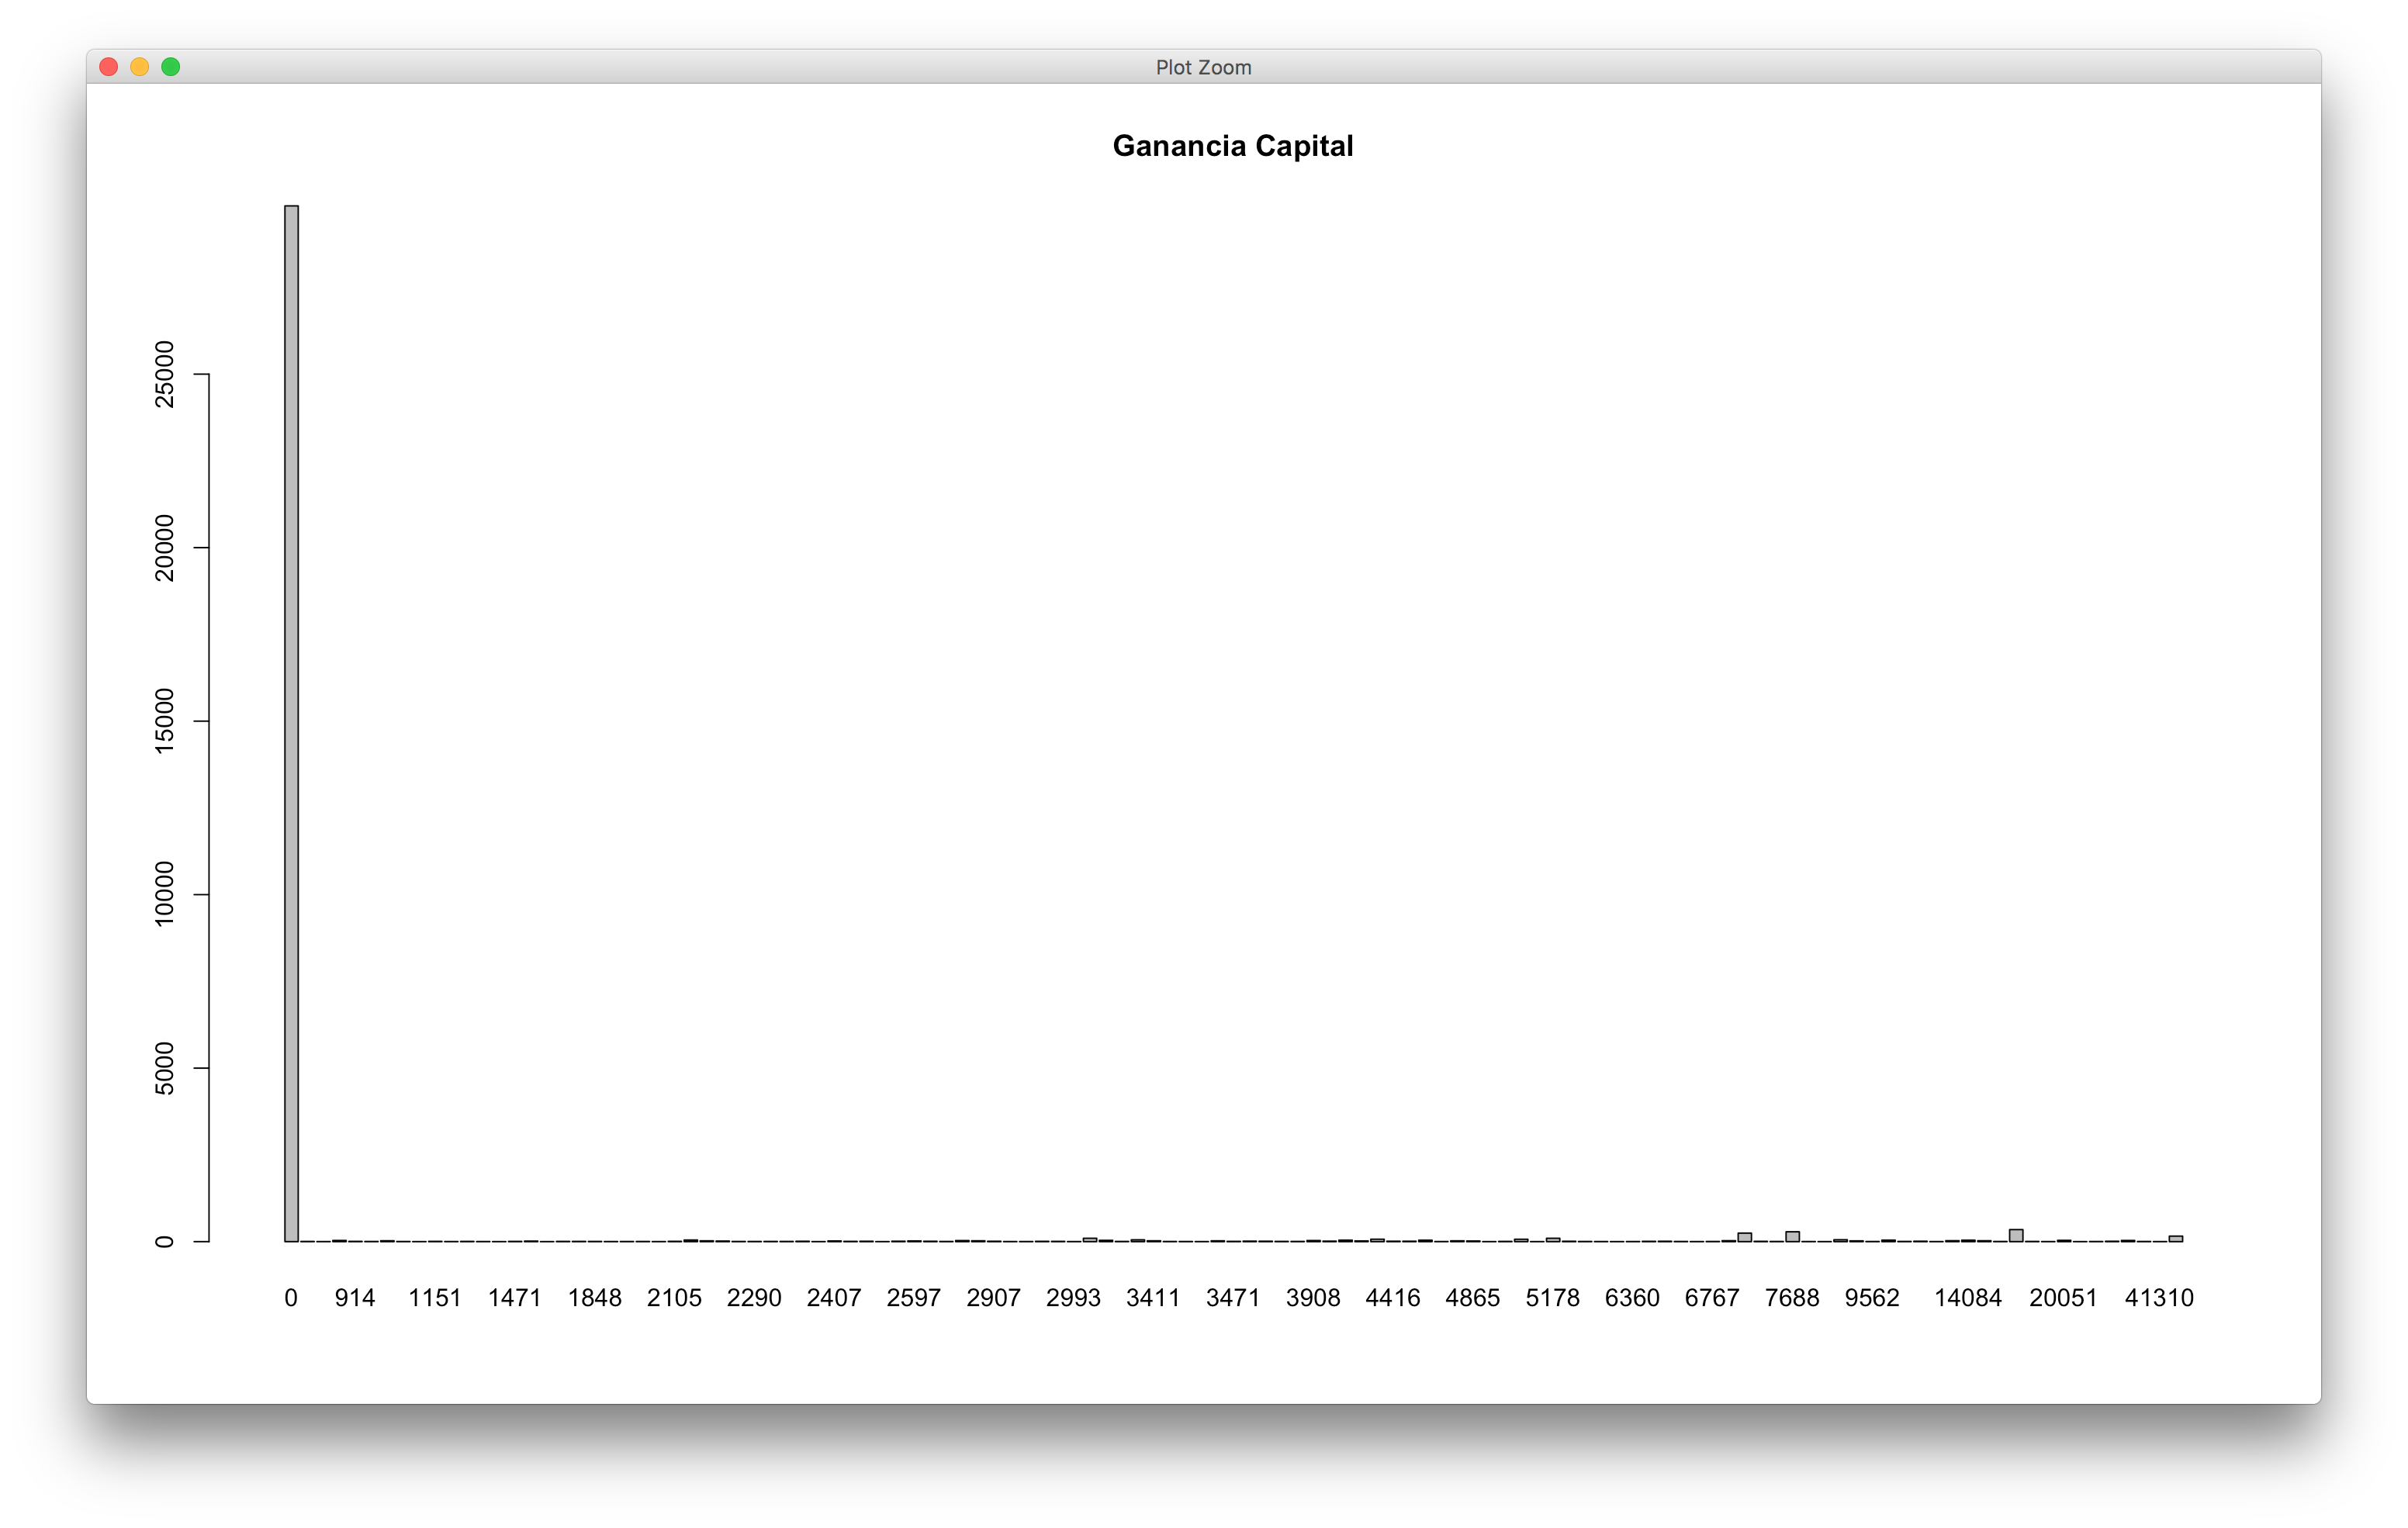
\includegraphics[scale=0.4]{graficas/gananciaCapital}}
 \end{center}
 \begin{center}
   \hbox{\hspace{-5.8em}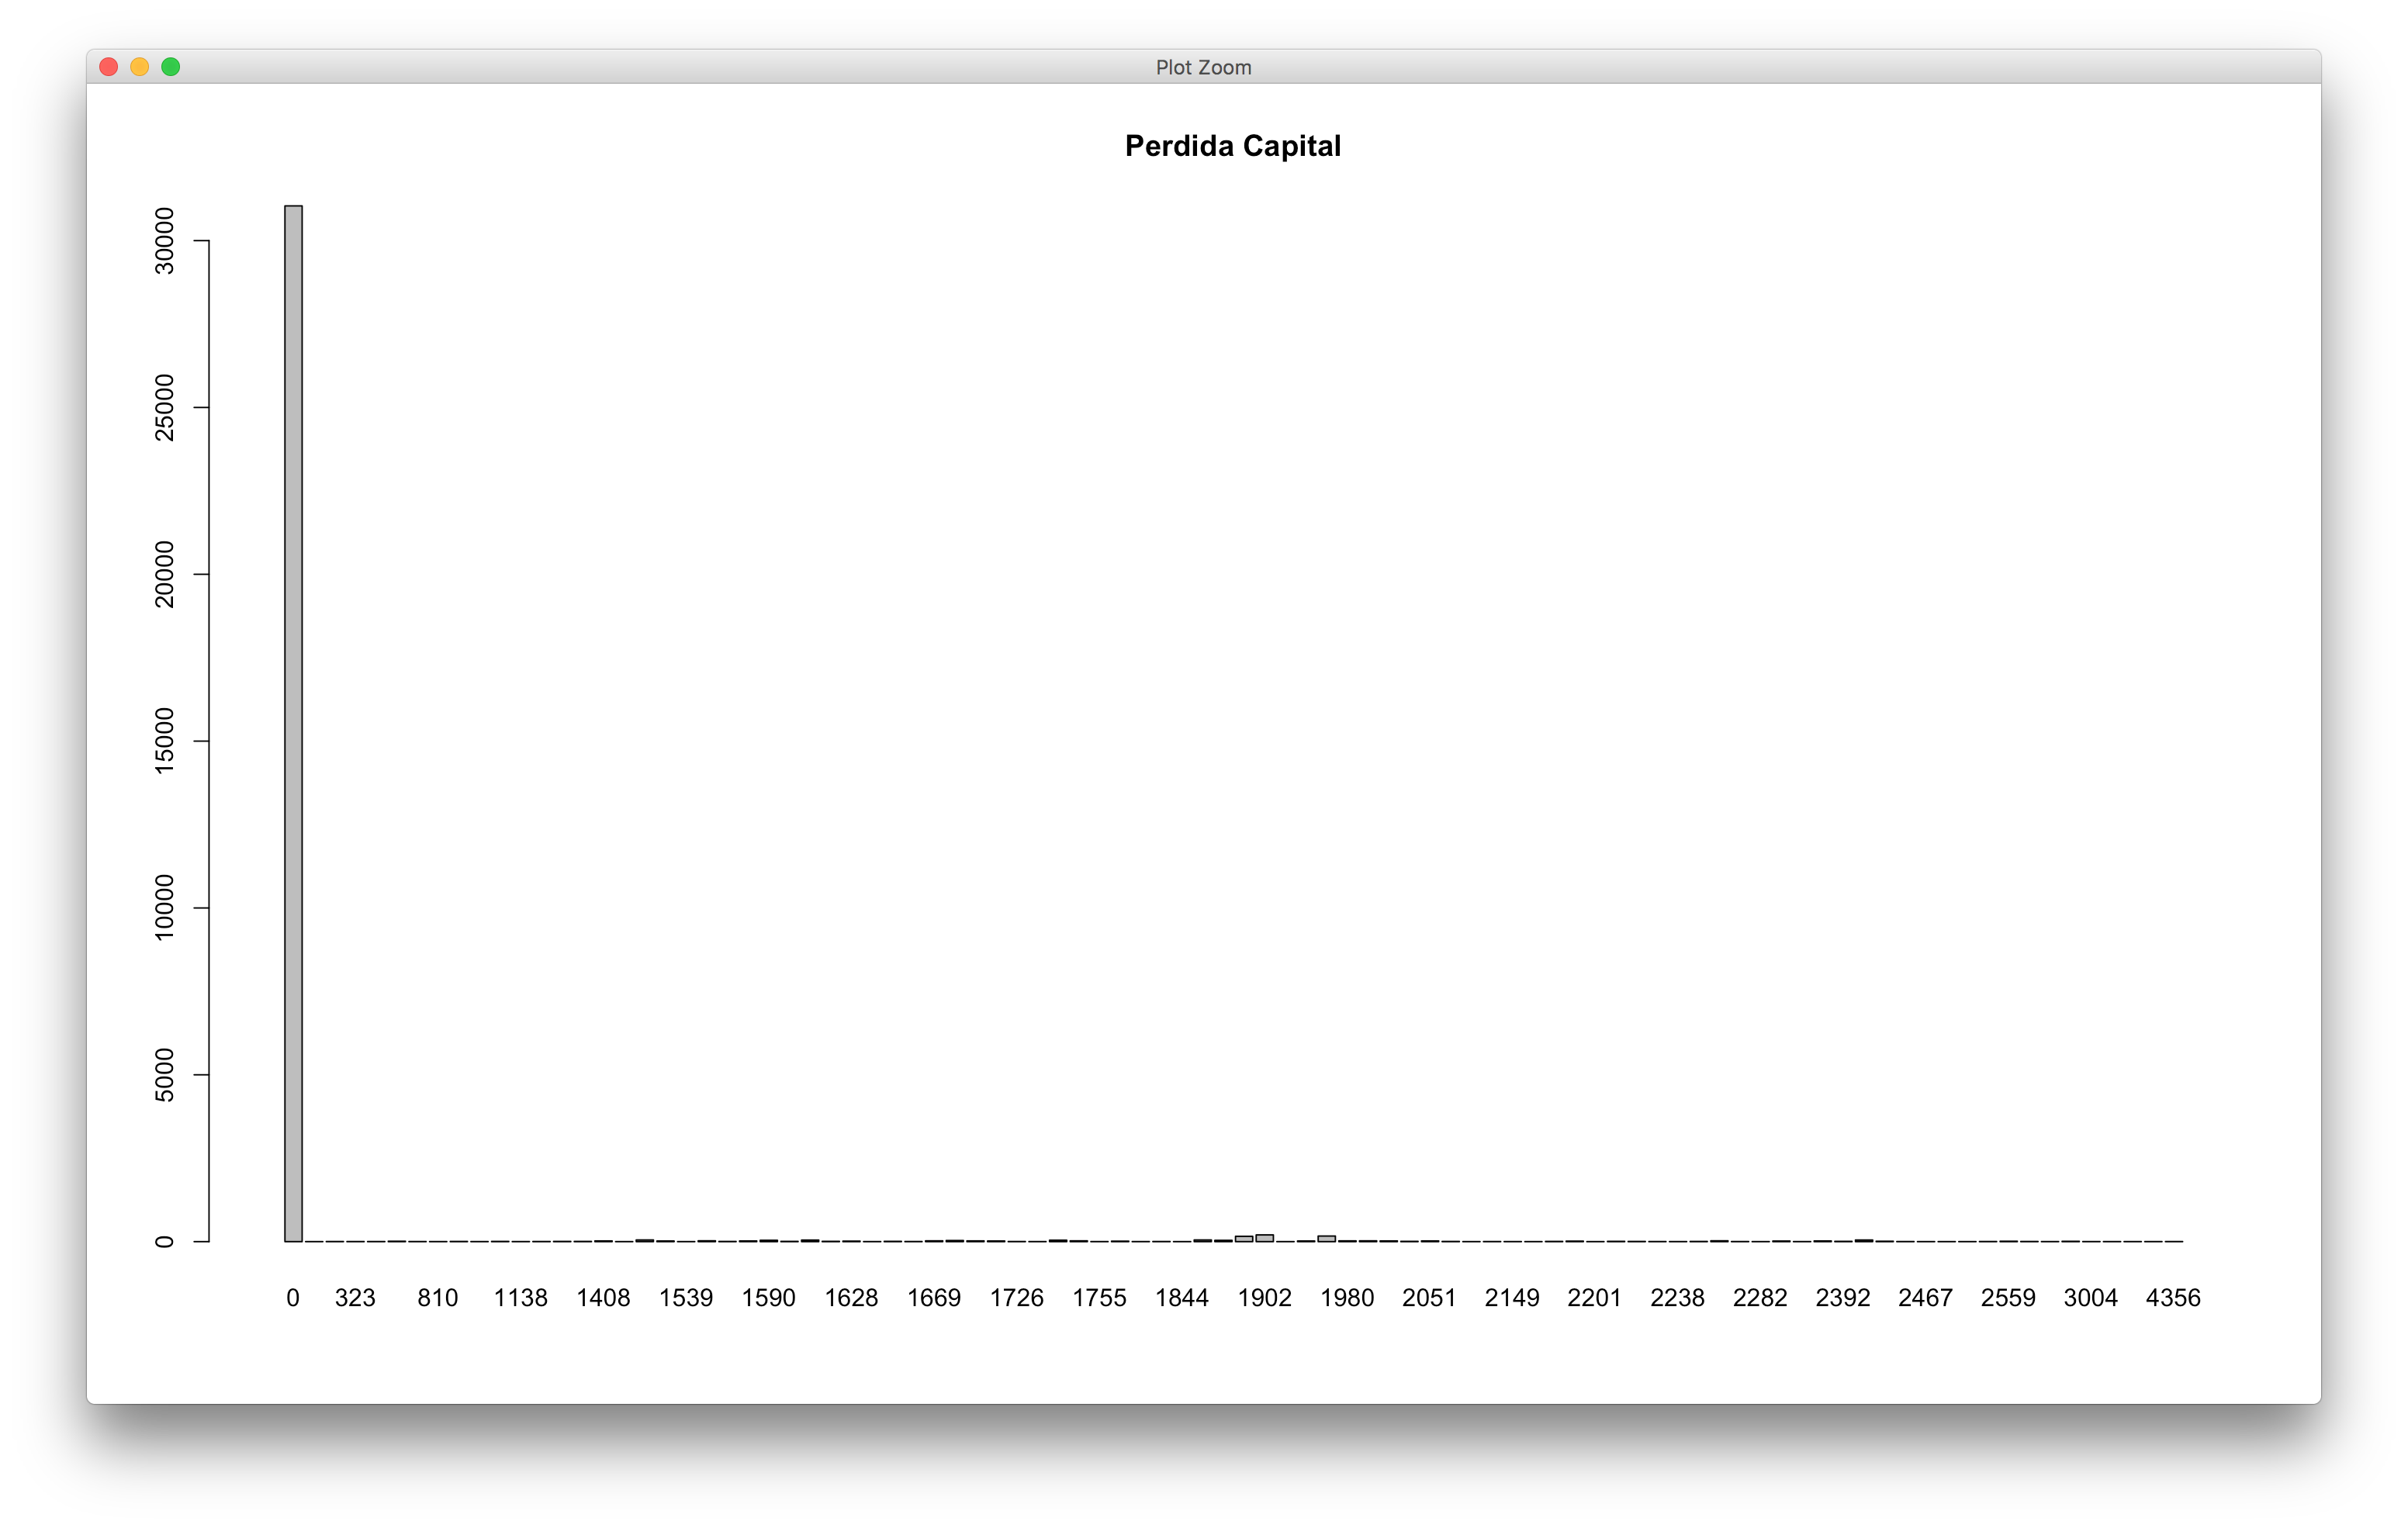
\includegraphics[scale=0.4]{graficas/perdidaCapital}}
 \end{center}
 \begin{center}
   \hbox{\hspace{-5.8em}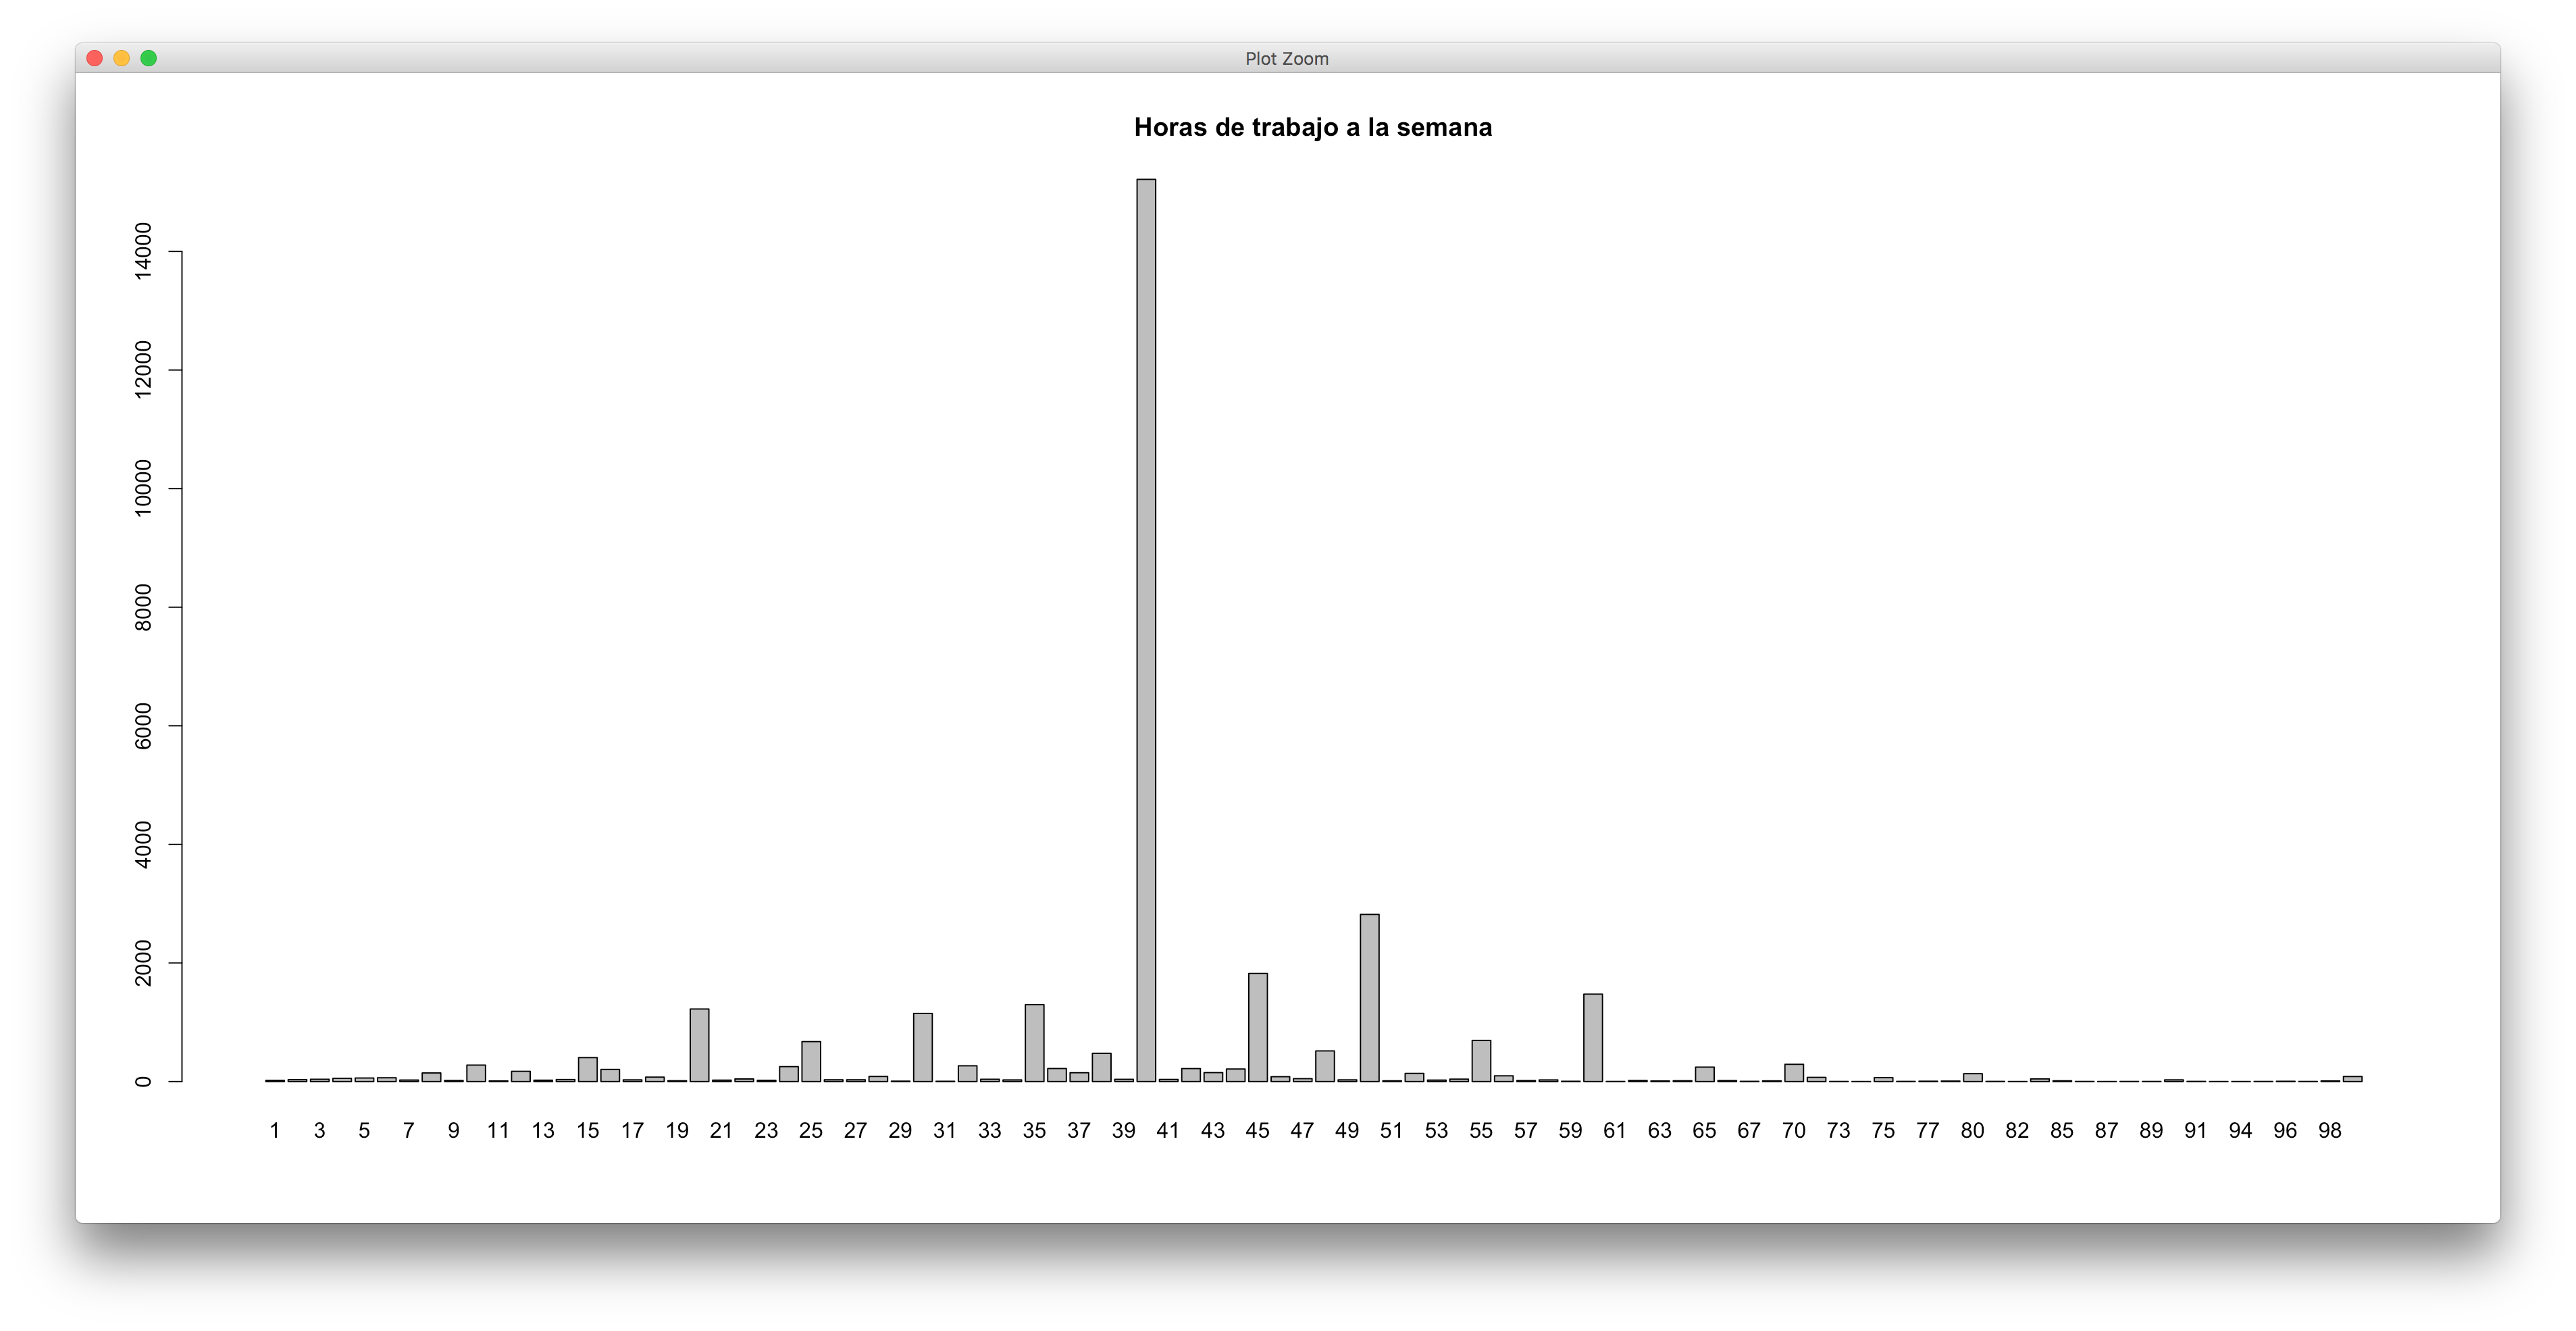
\includegraphics[scale=0.33]{graficas/horasALaSemana}}
 \end{center}
 \begin{center}
   \hbox{\hspace{-5.8em}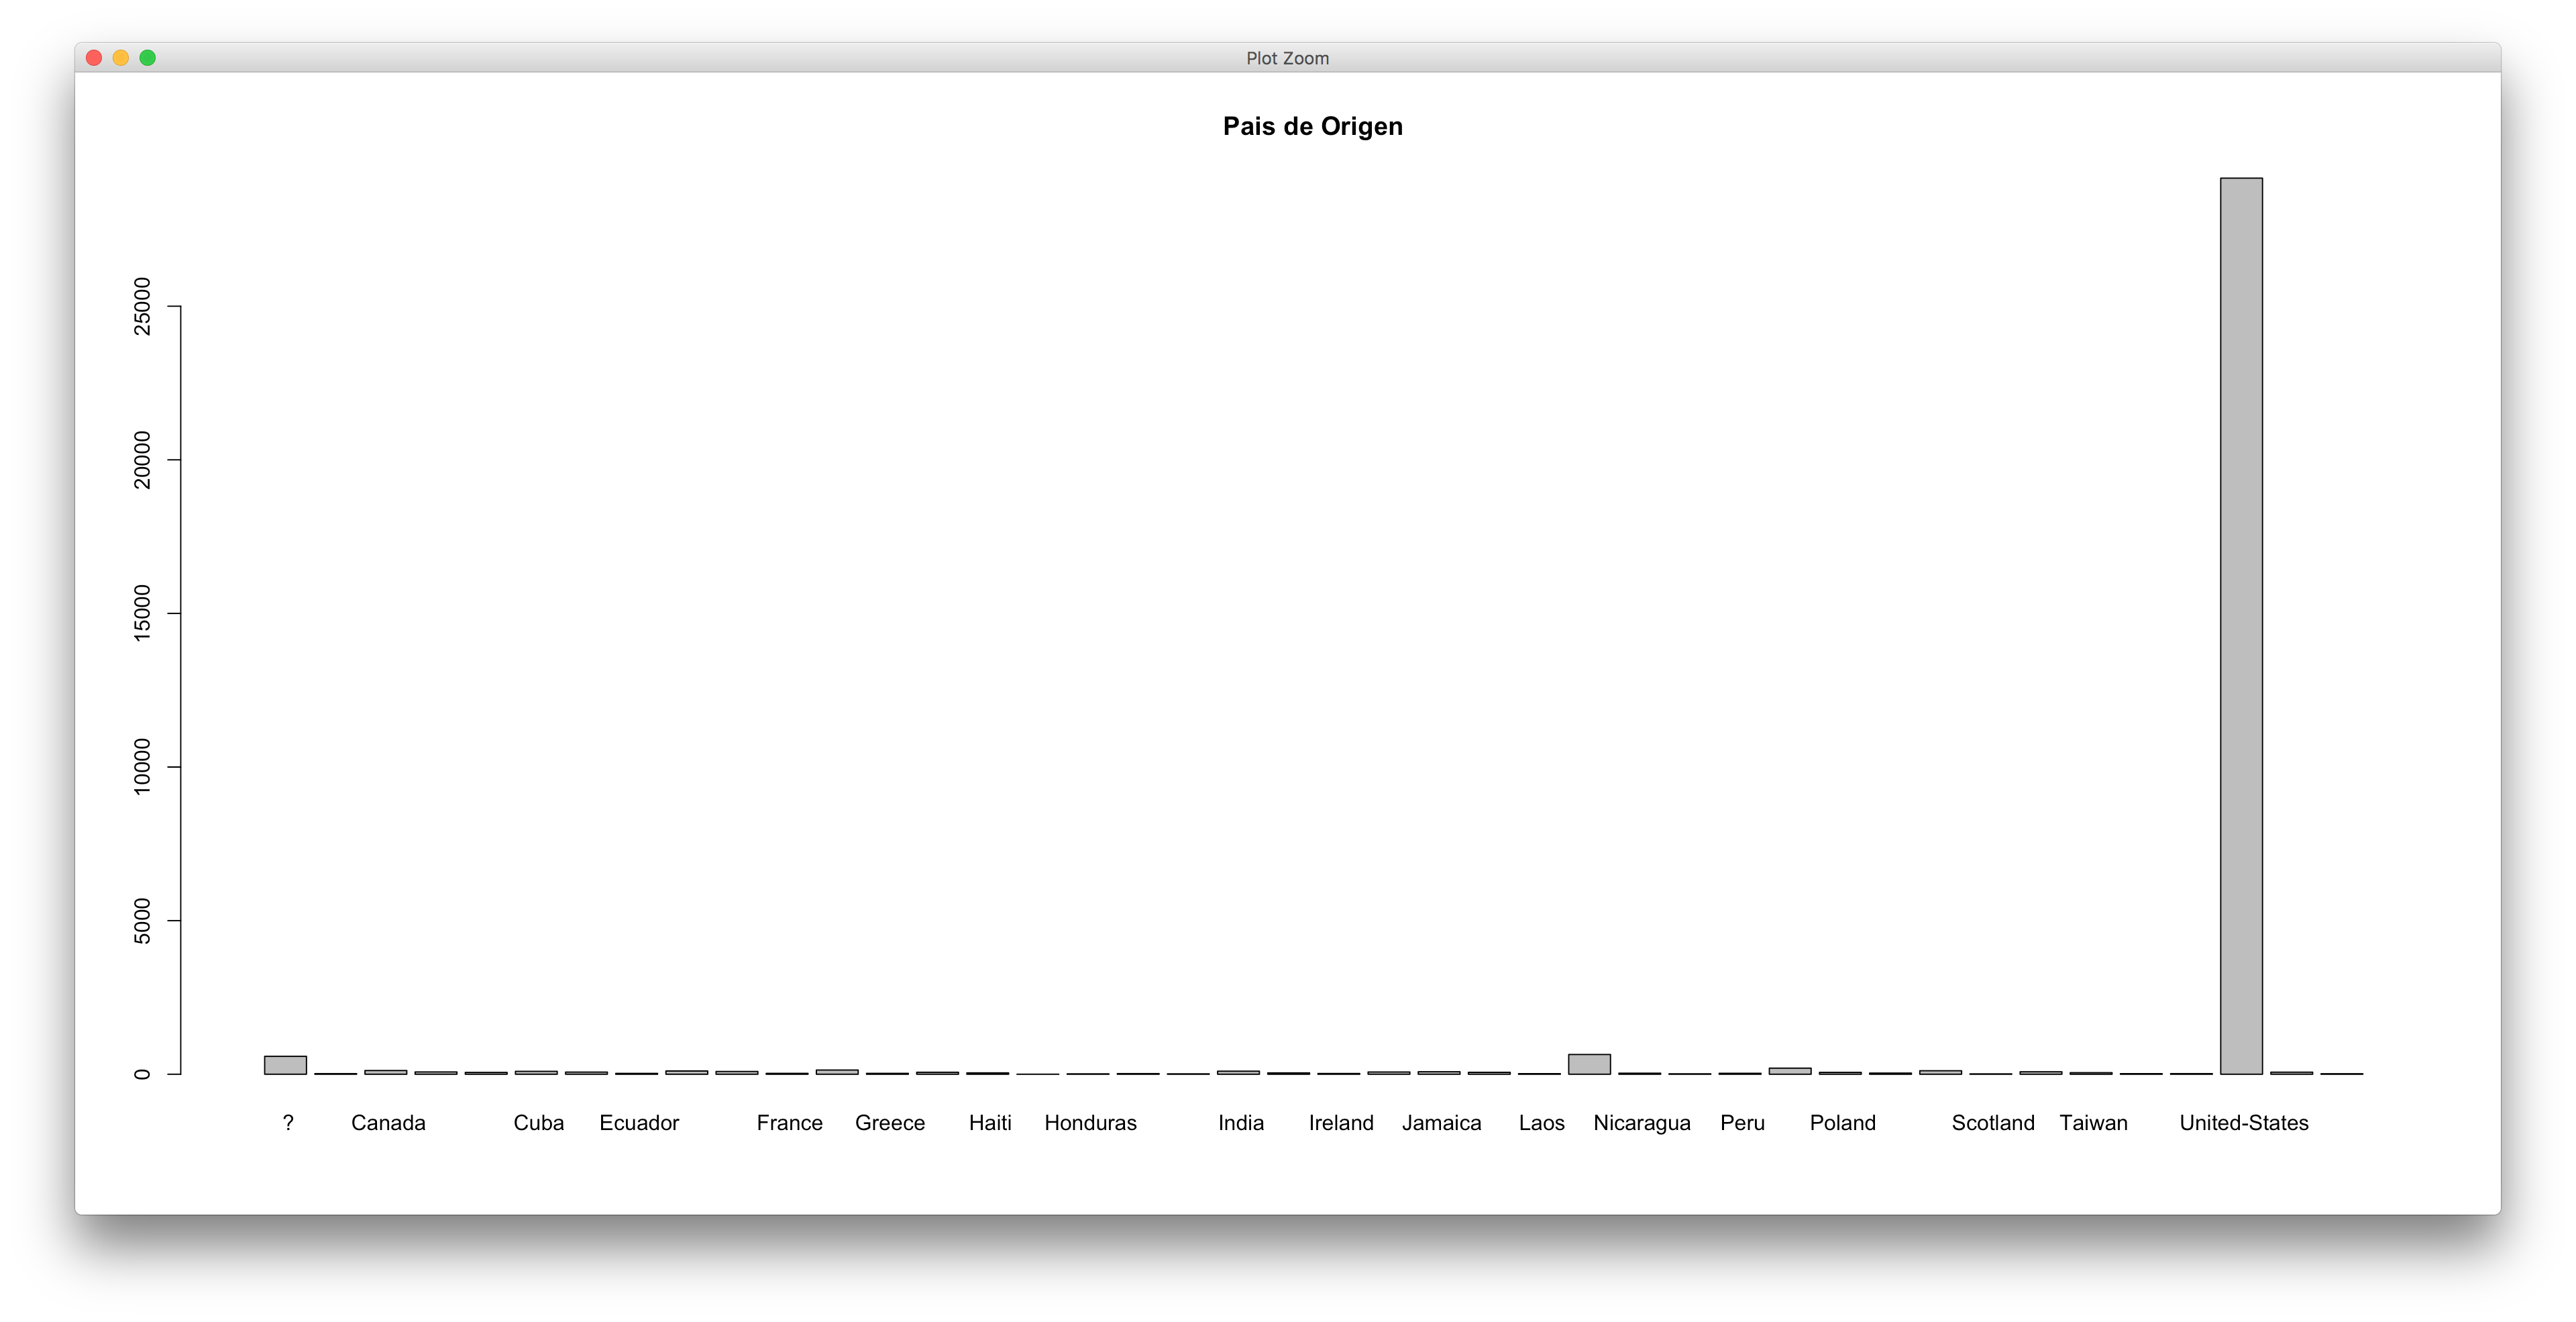
\includegraphics[scale=0.33]{graficas/paisDeOrigen}}
 \end{center}
 \begin{center}
   \hbox{\hspace{-5.8em}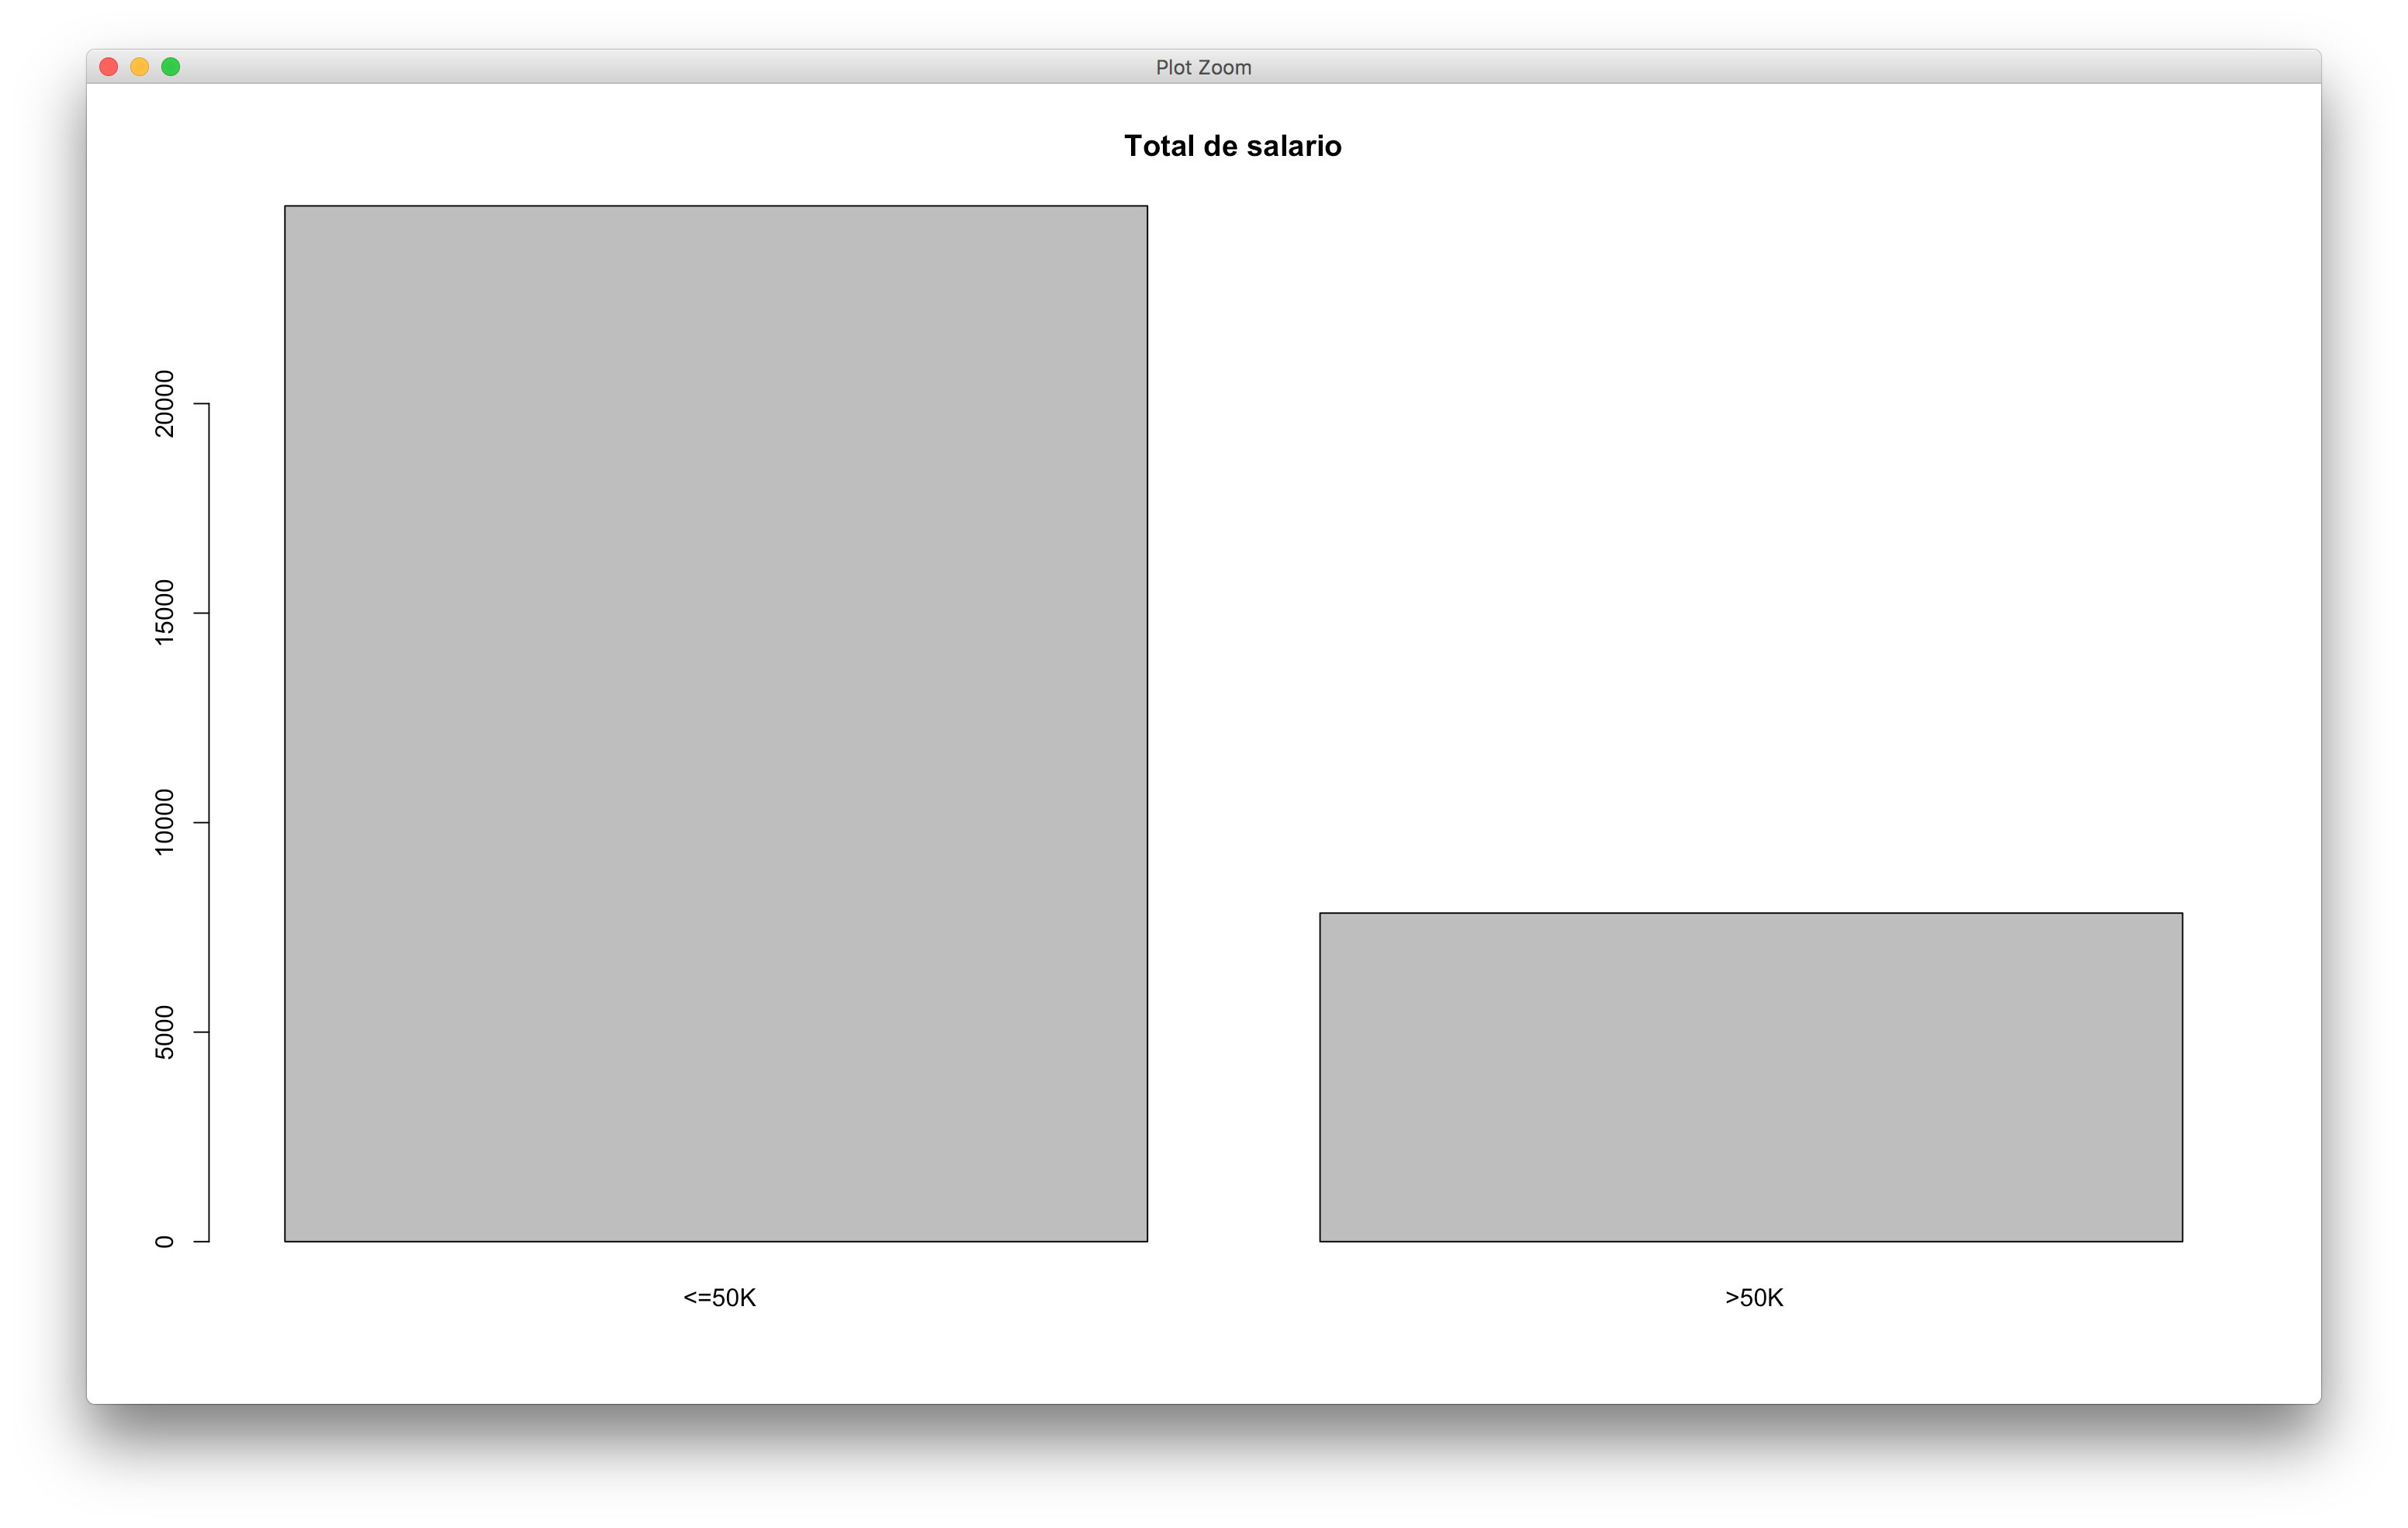
\includegraphics[scale=0.4]{graficas/totalDeSalario}}
 \end{center}

 Después de observar detalladamente estas gráficas pudimos observar que los atributos que más se repiten son los siguientes: son hombres con edad de 23 a 40 años, los cuales trabajan en el sector privado, con un grado de educación de preparatoria, están casados, son de raza blanca, trabajan 40 horas a la semana y su país de origen es Estados Unidos.

\subsection{Por Parejas}
  \begin{center}
    \hbox{\hspace{-5.5em}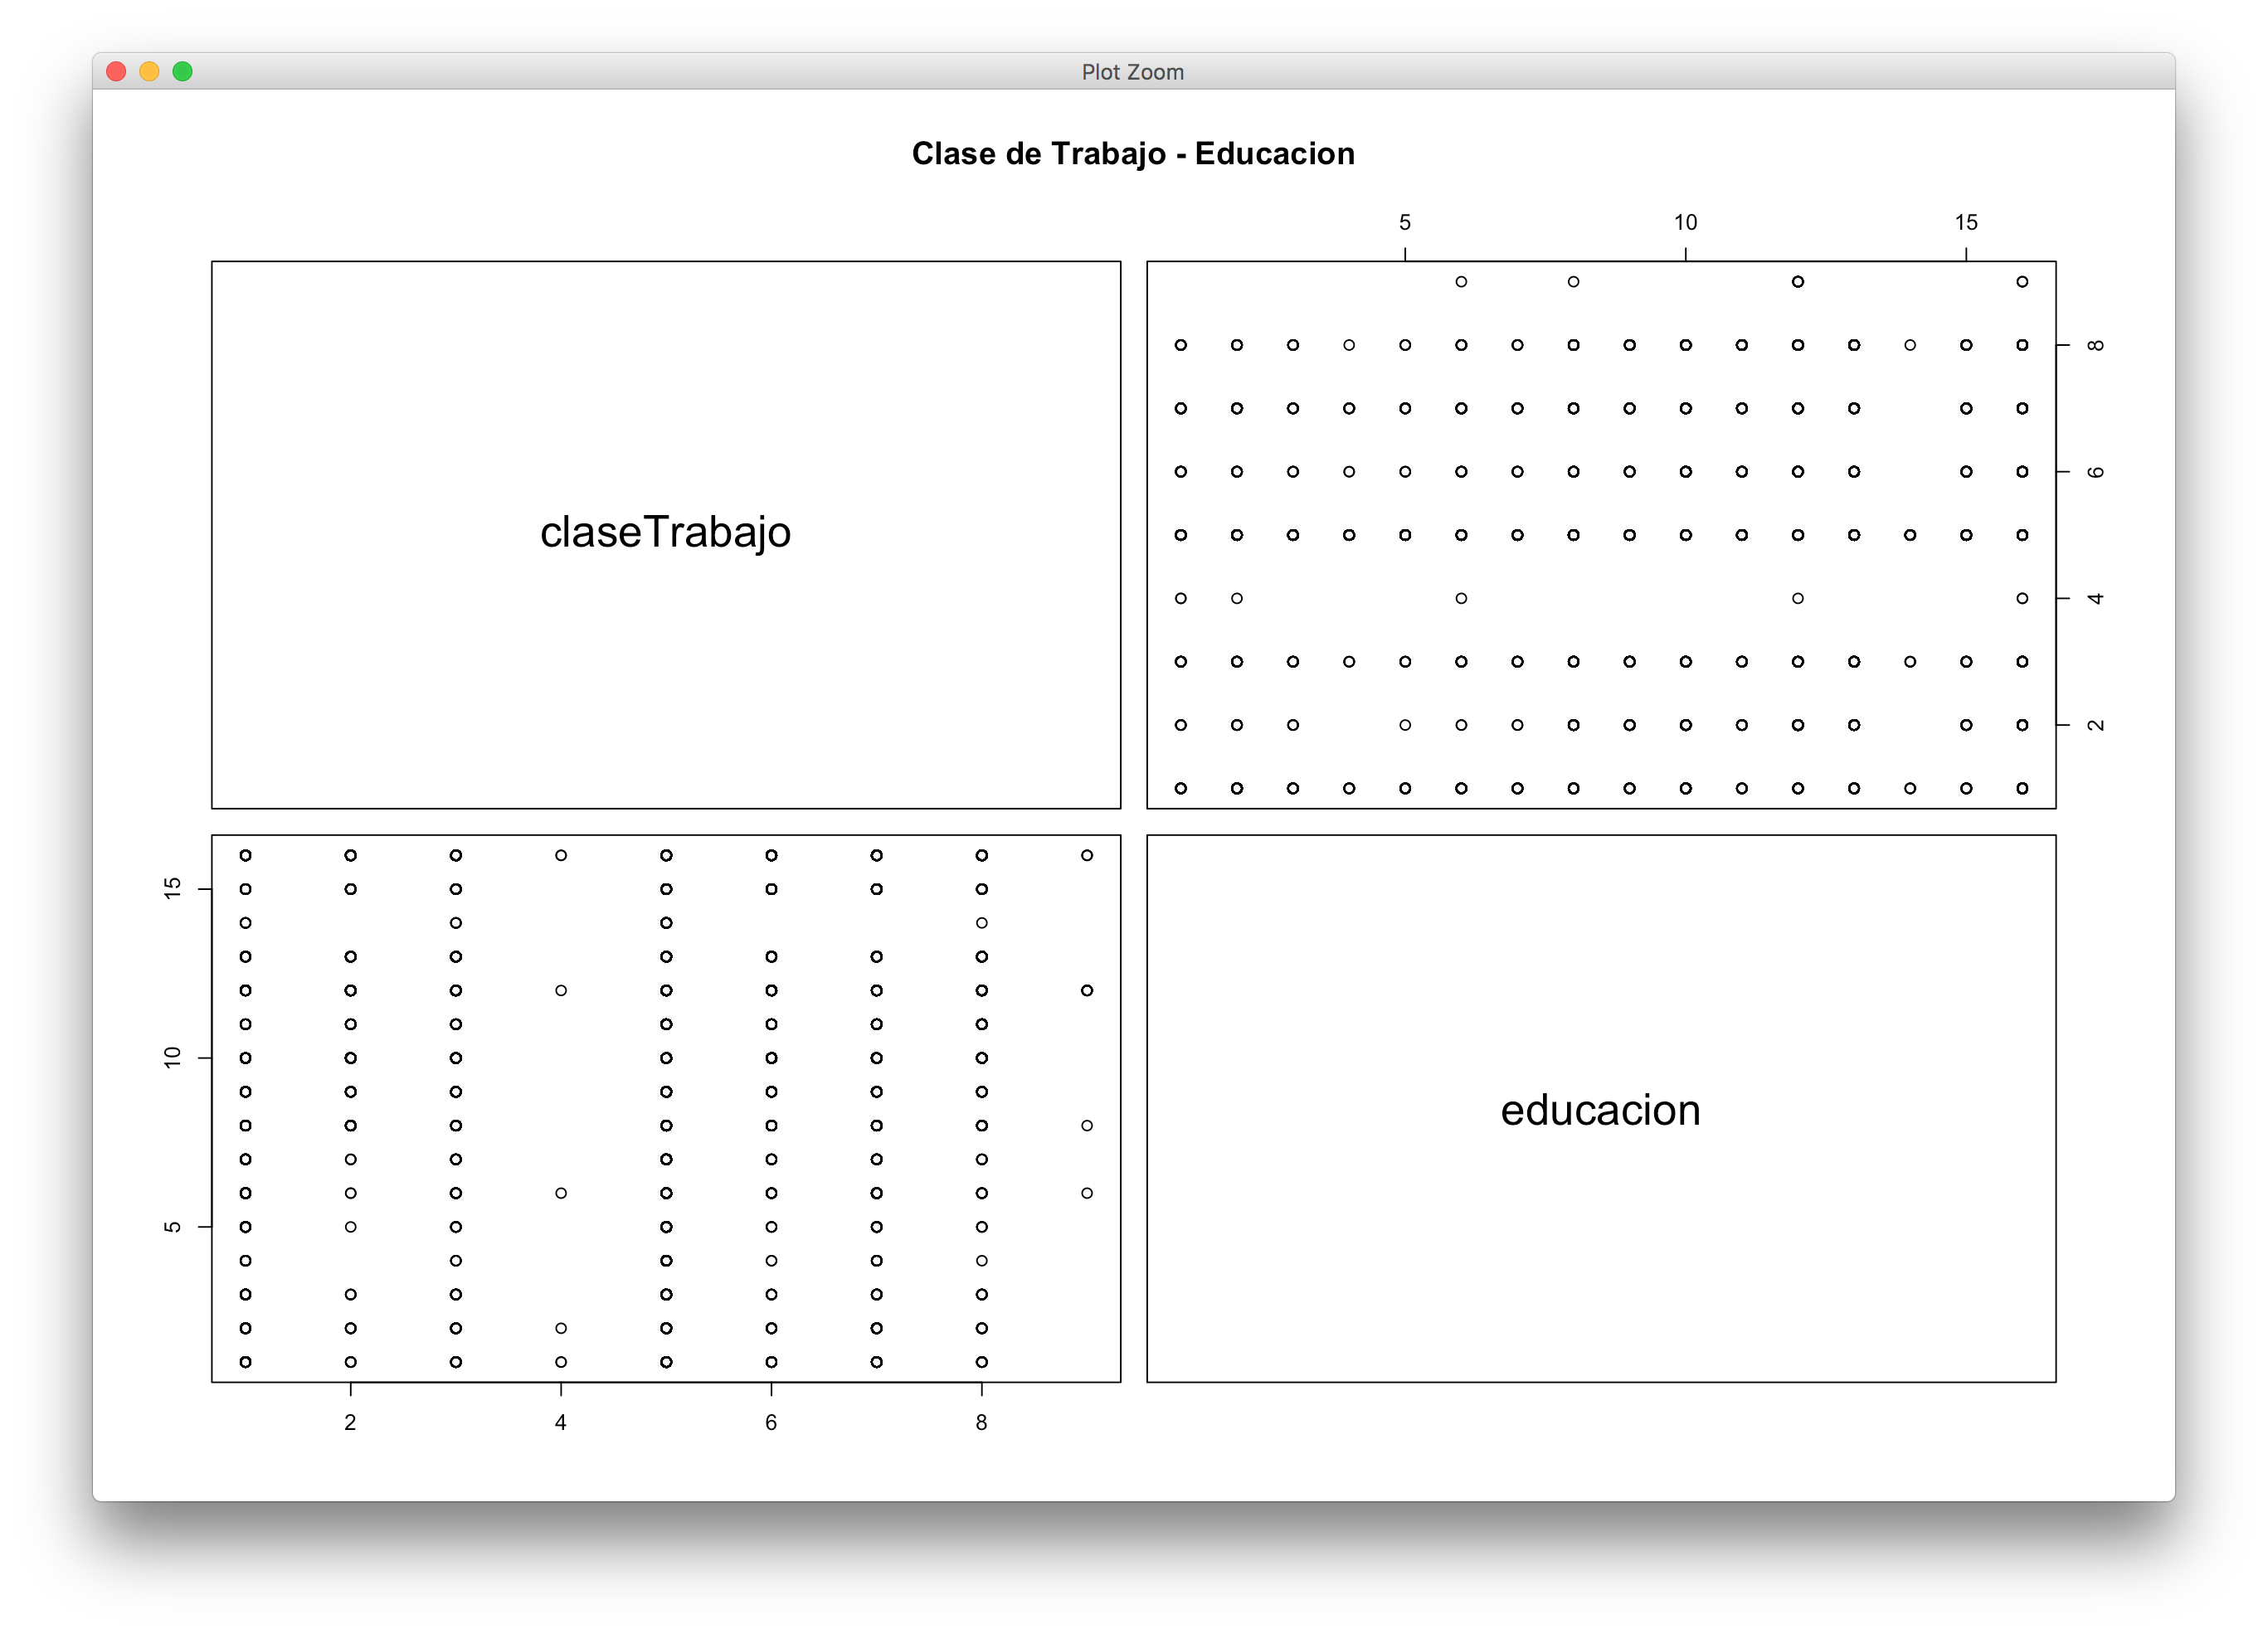
\includegraphics[scale=0.45]{graficas/ClaseTrabEdu}}
  \end{center}
  \begin{center}
    \hbox{\hspace{-5.5em}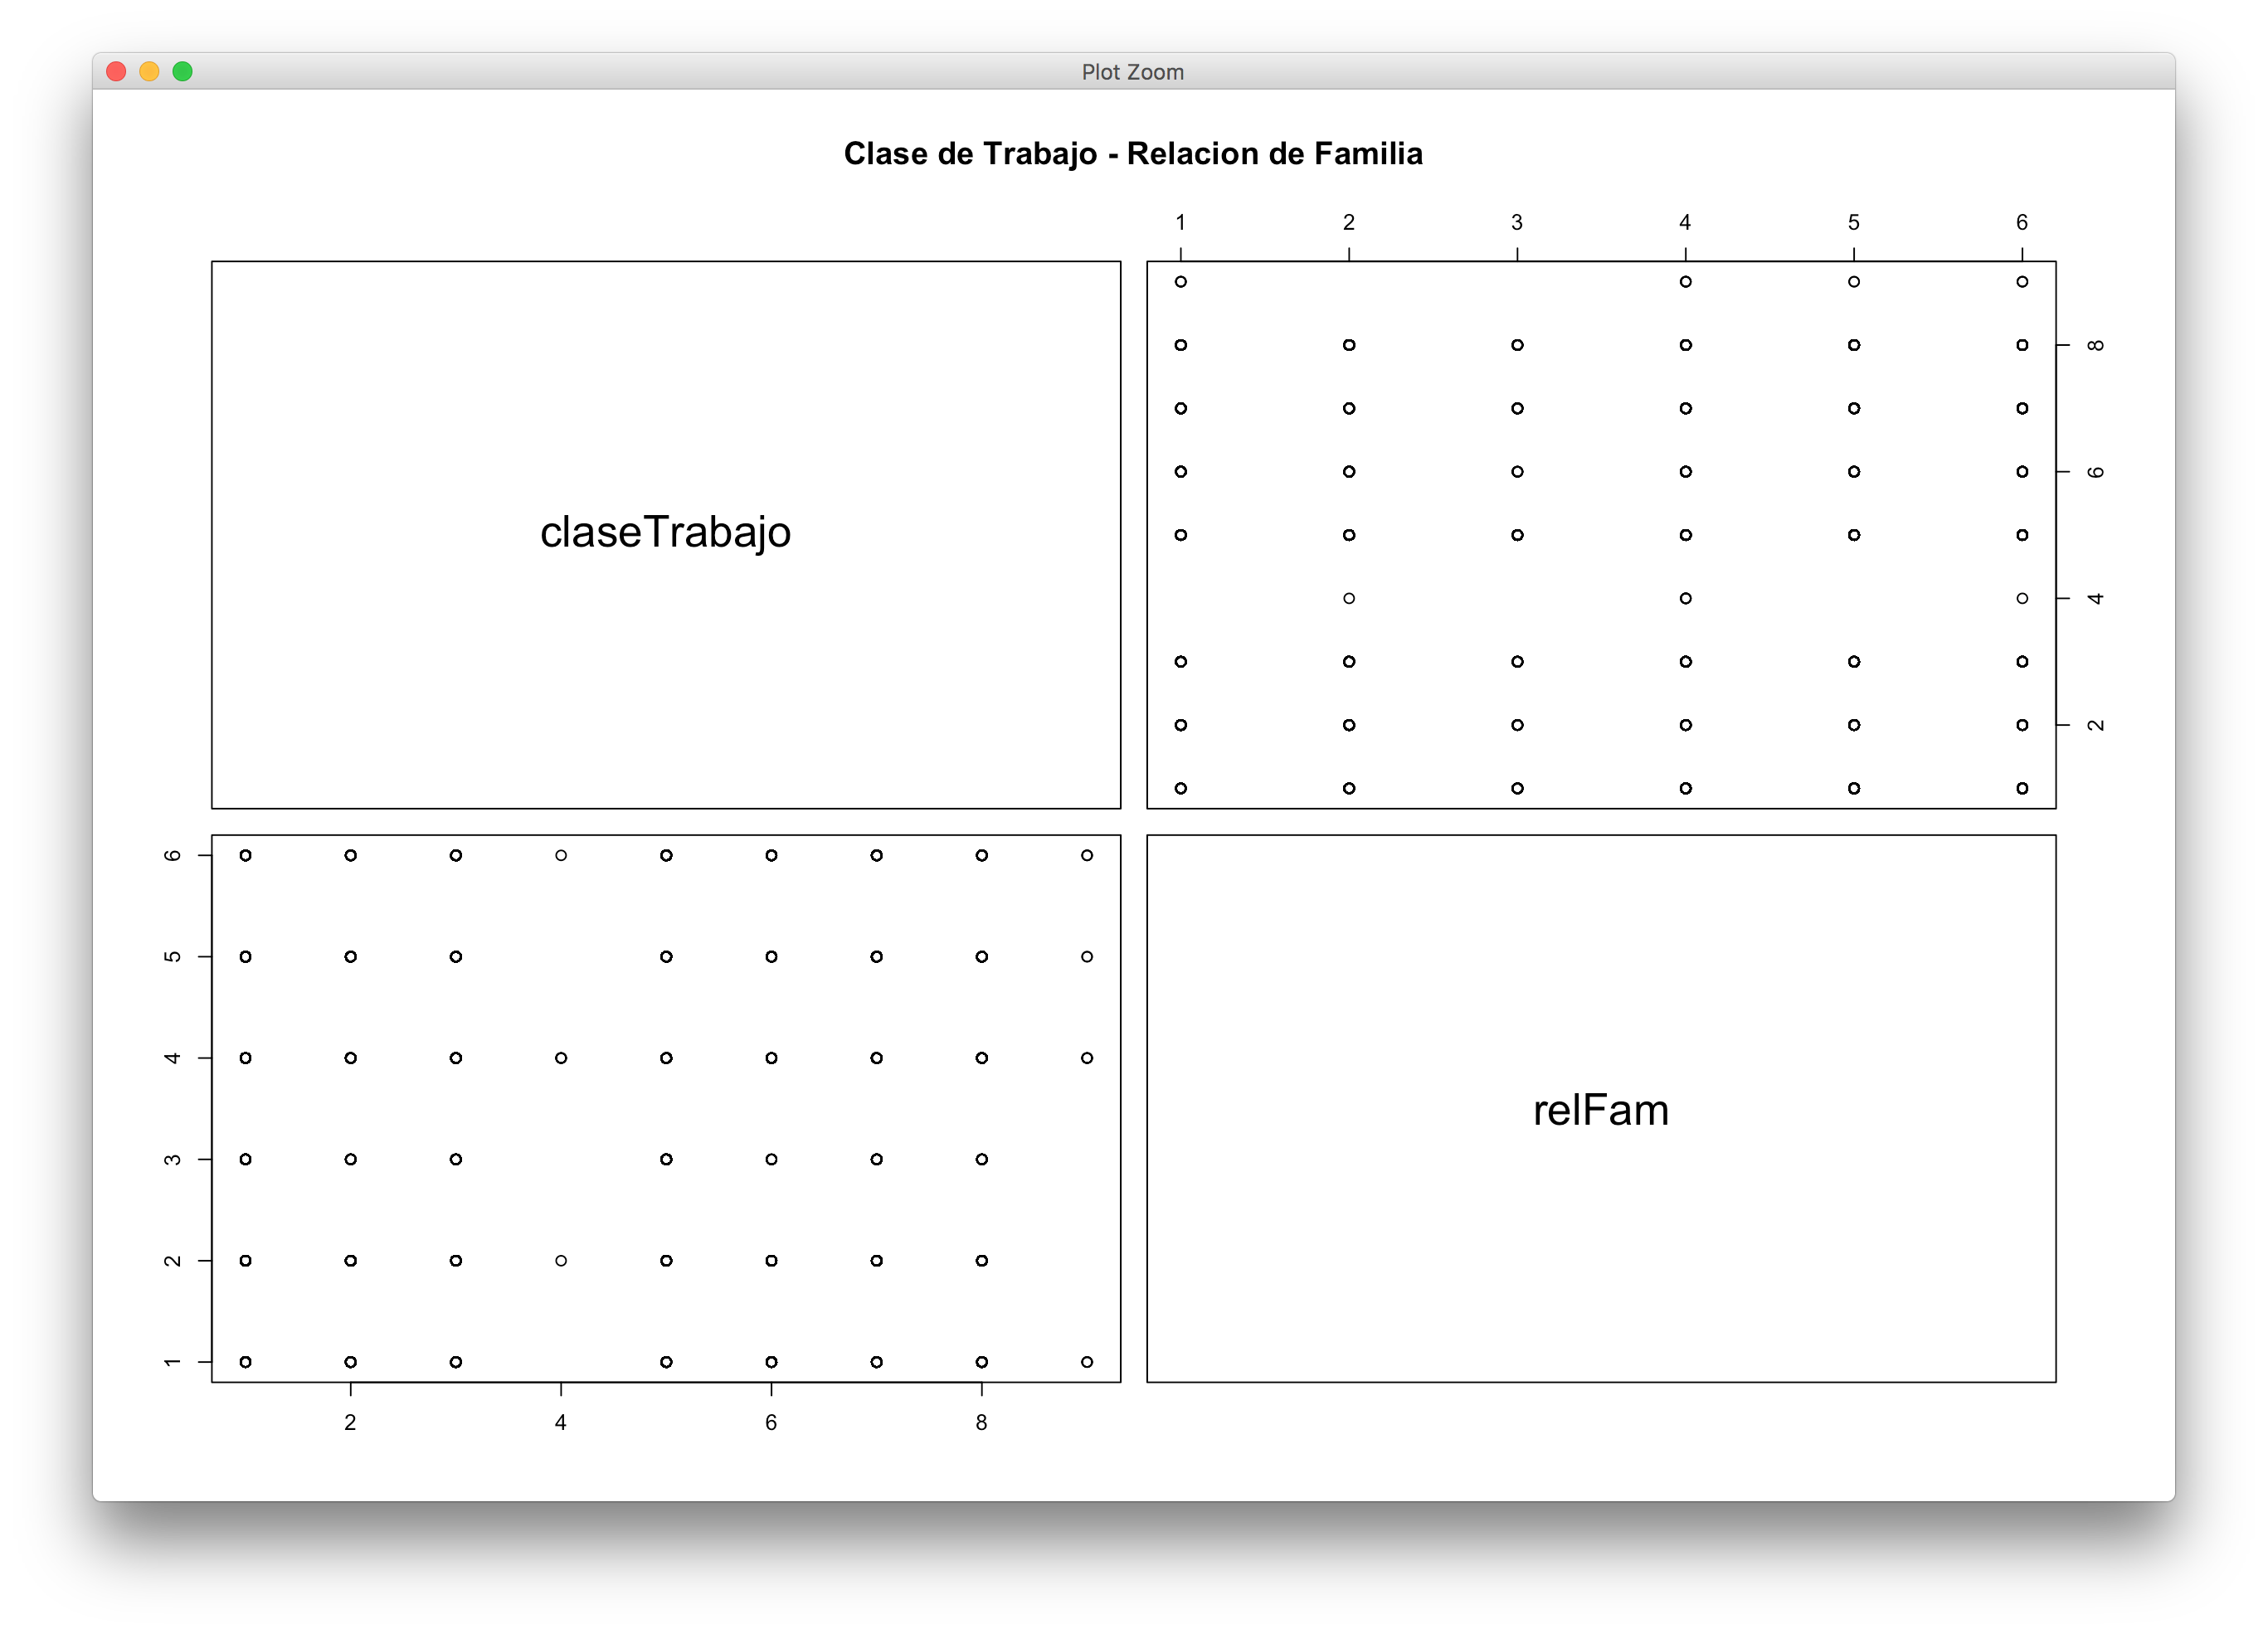
\includegraphics[scale=0.45]{graficas/claseTrabjRelSem}}
  \end{center}
  \begin{center}
    \hbox{\hspace{-5.5em}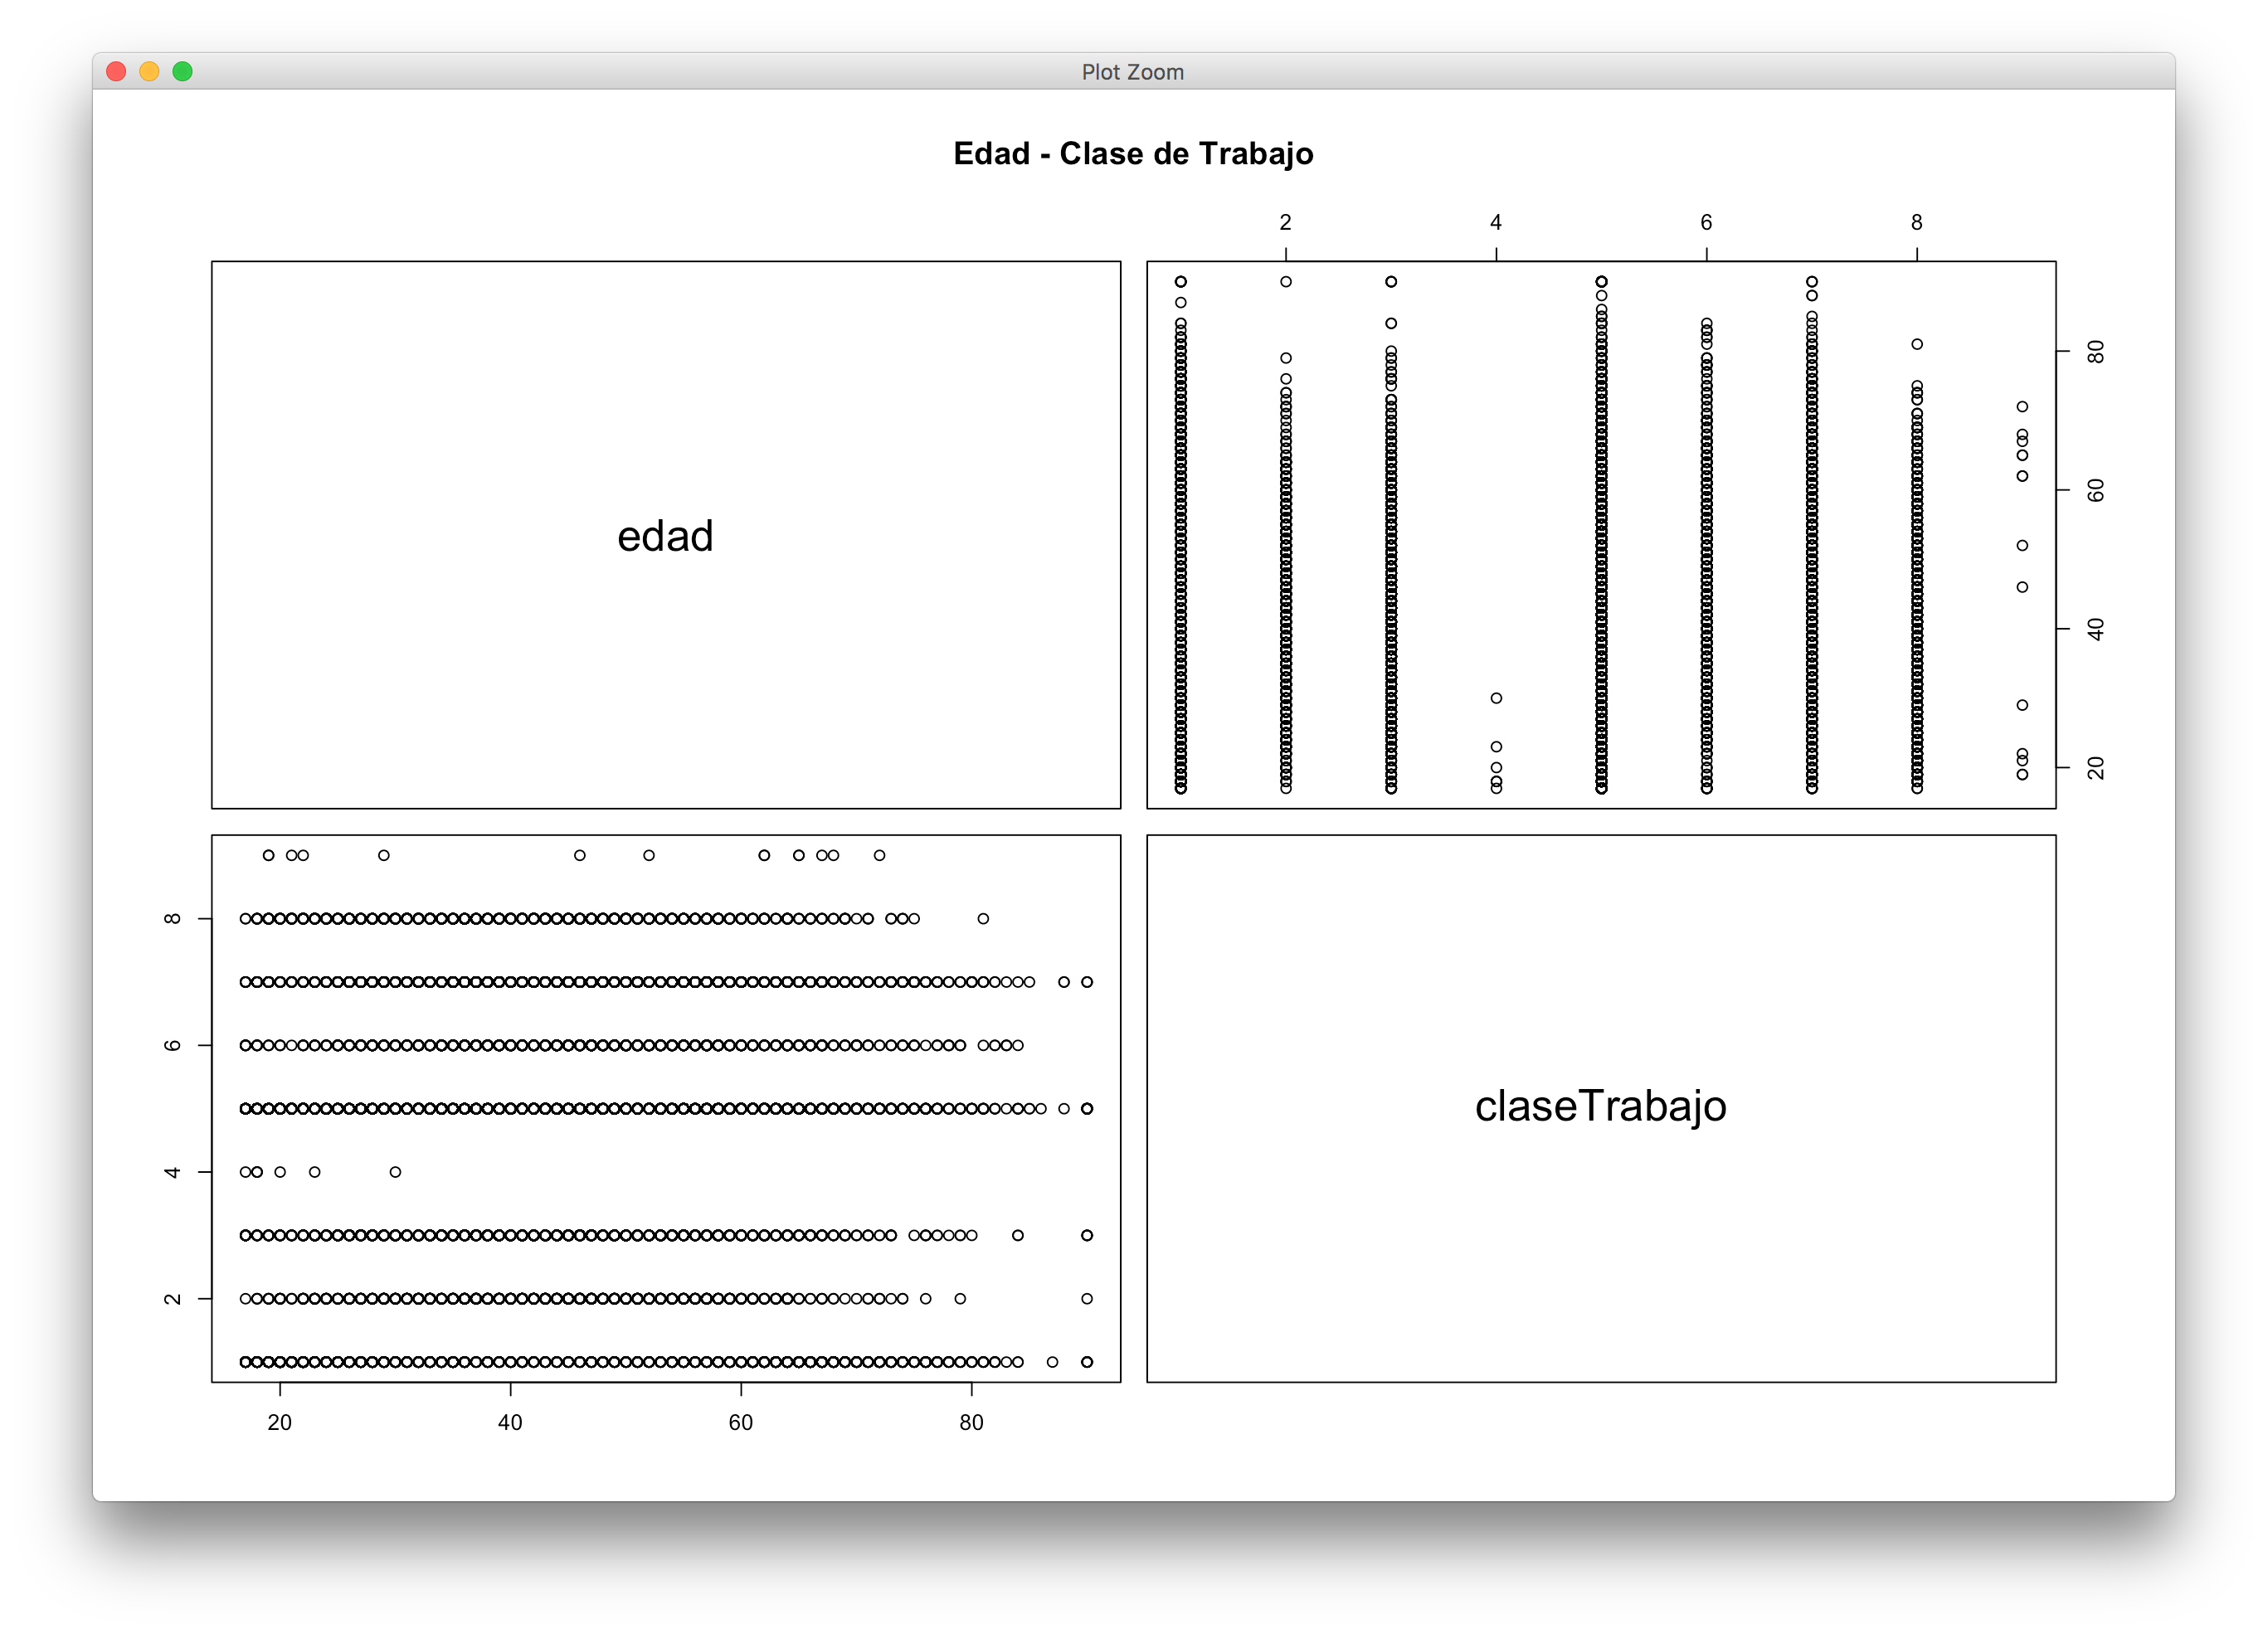
\includegraphics[scale=0.45]{graficas/edadClaseTrab}}
  \end{center}
  \begin{center}
    \hbox{\hspace{-5.5em}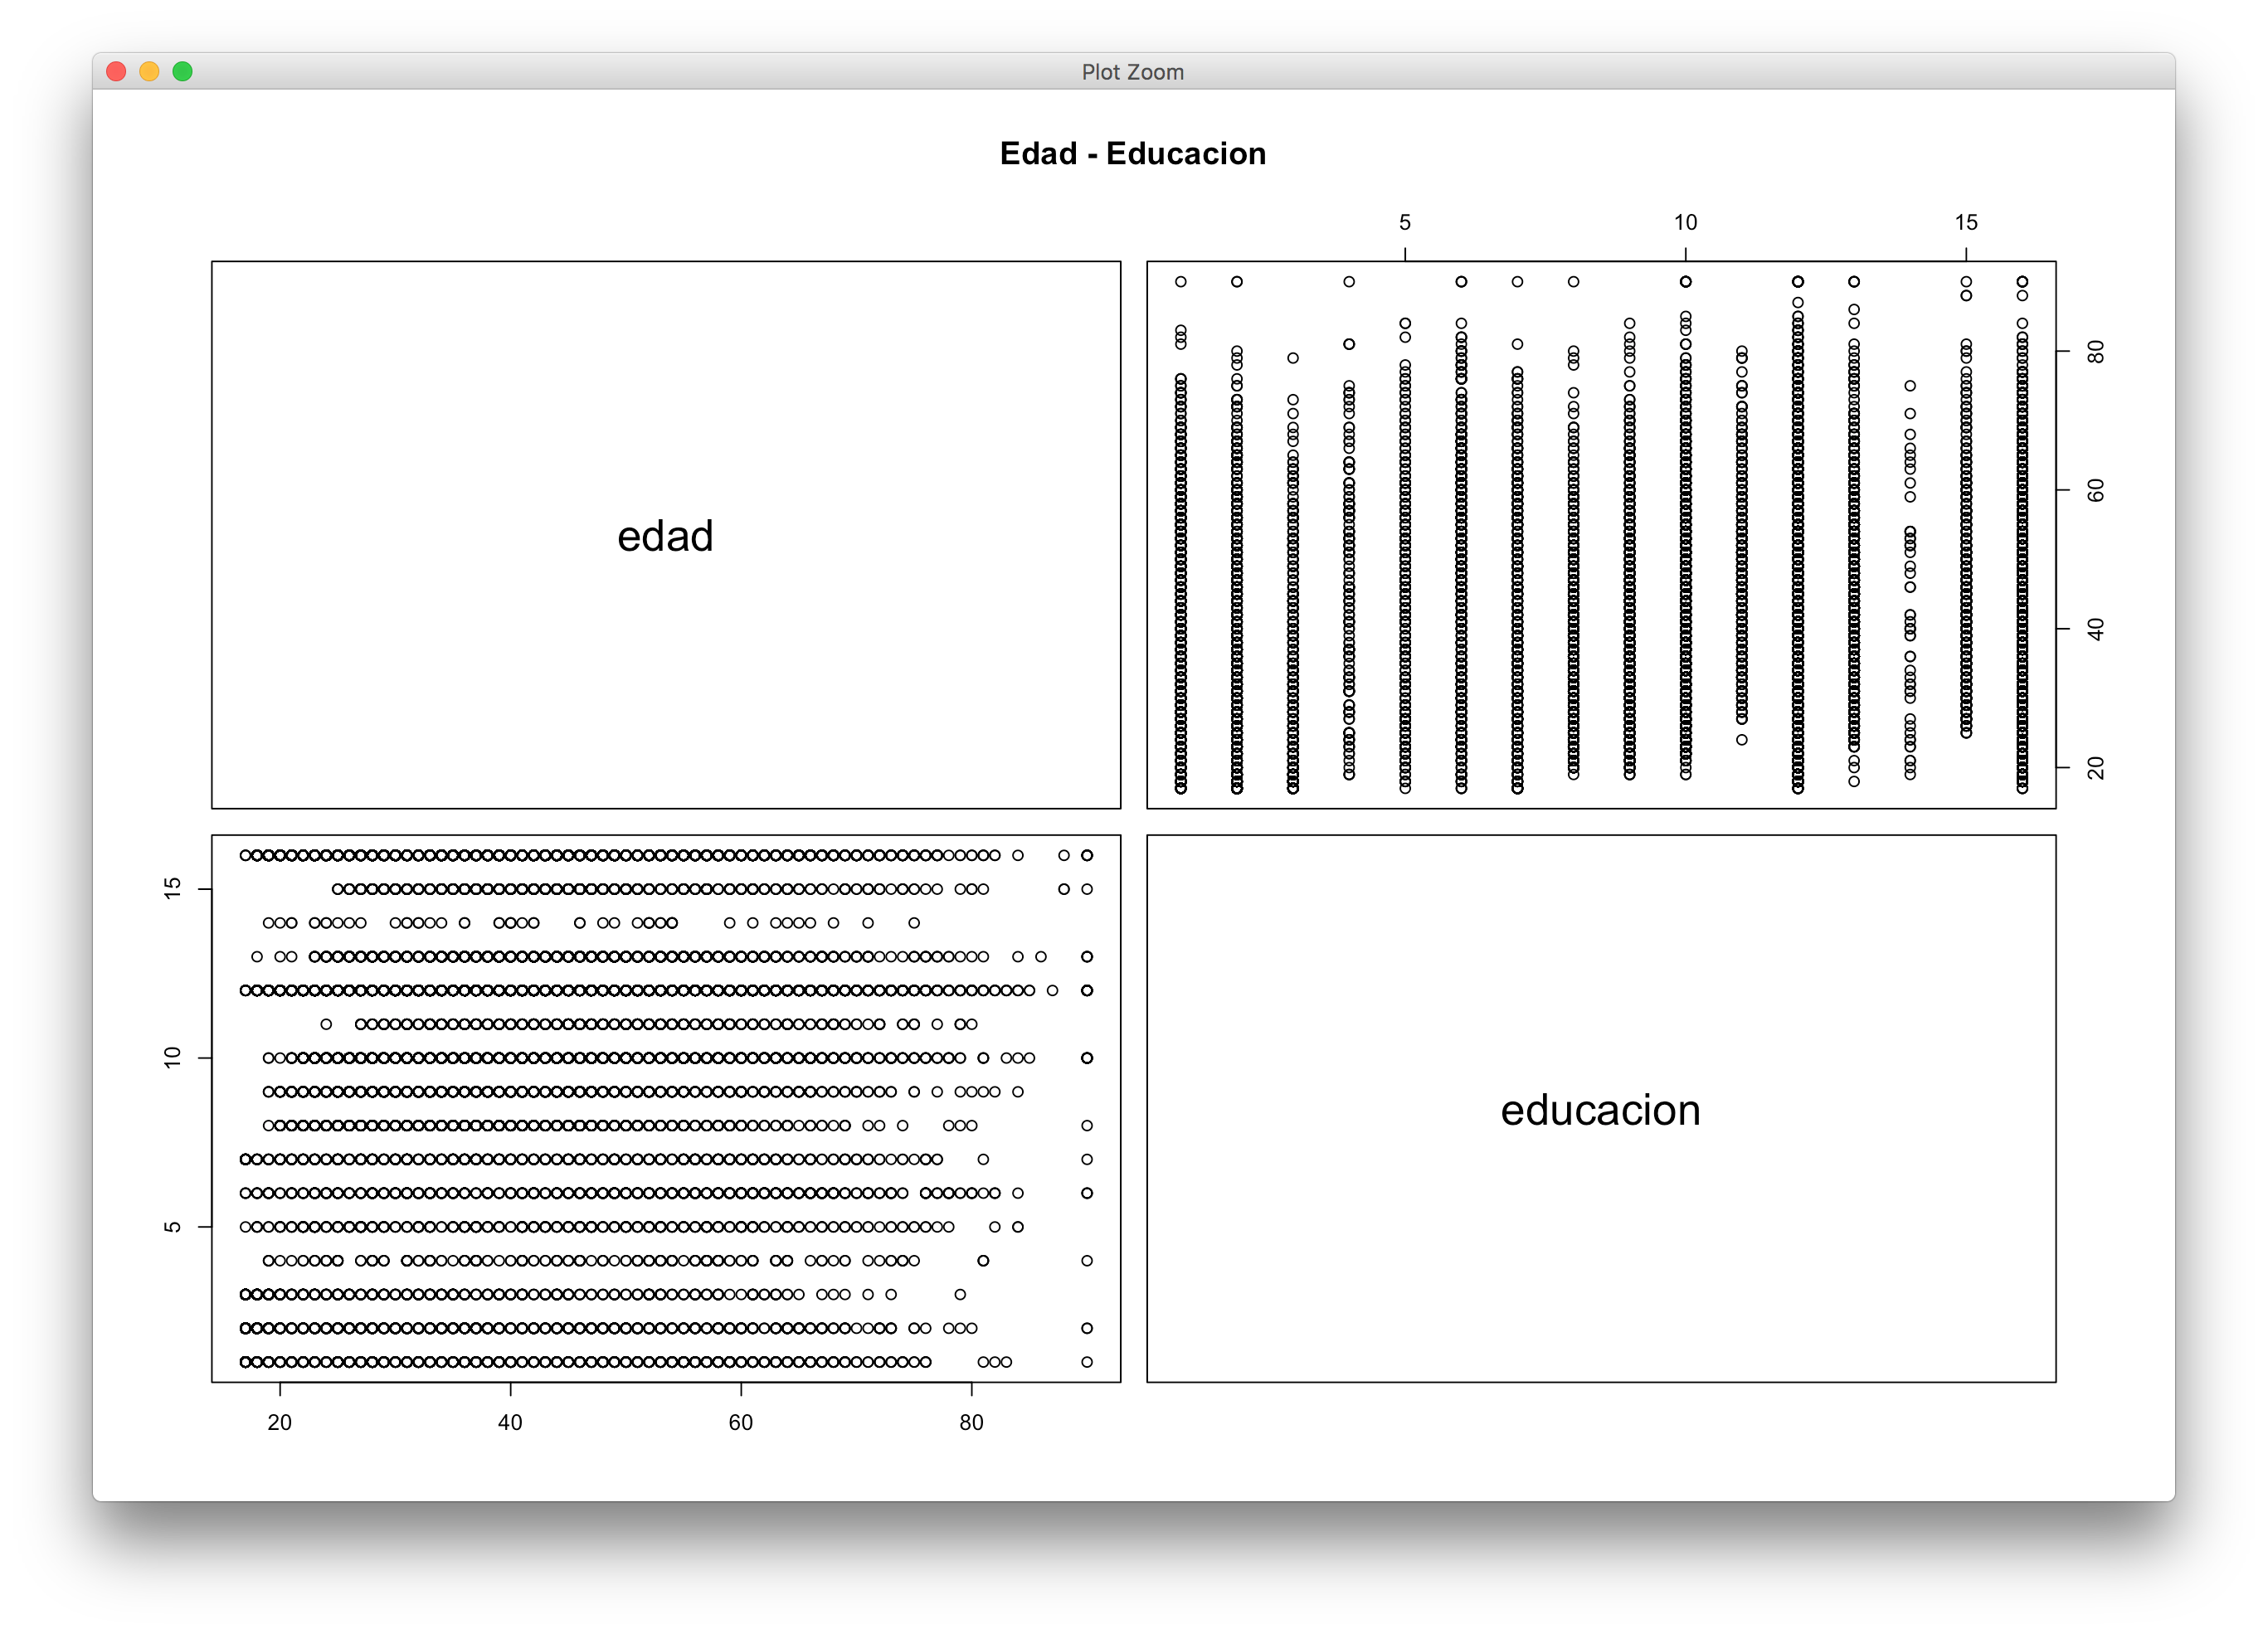
\includegraphics[scale=0.45]{graficas/edadEdu}}
  \end{center}
  \begin{center}
    \hbox{\hspace{-5.5em}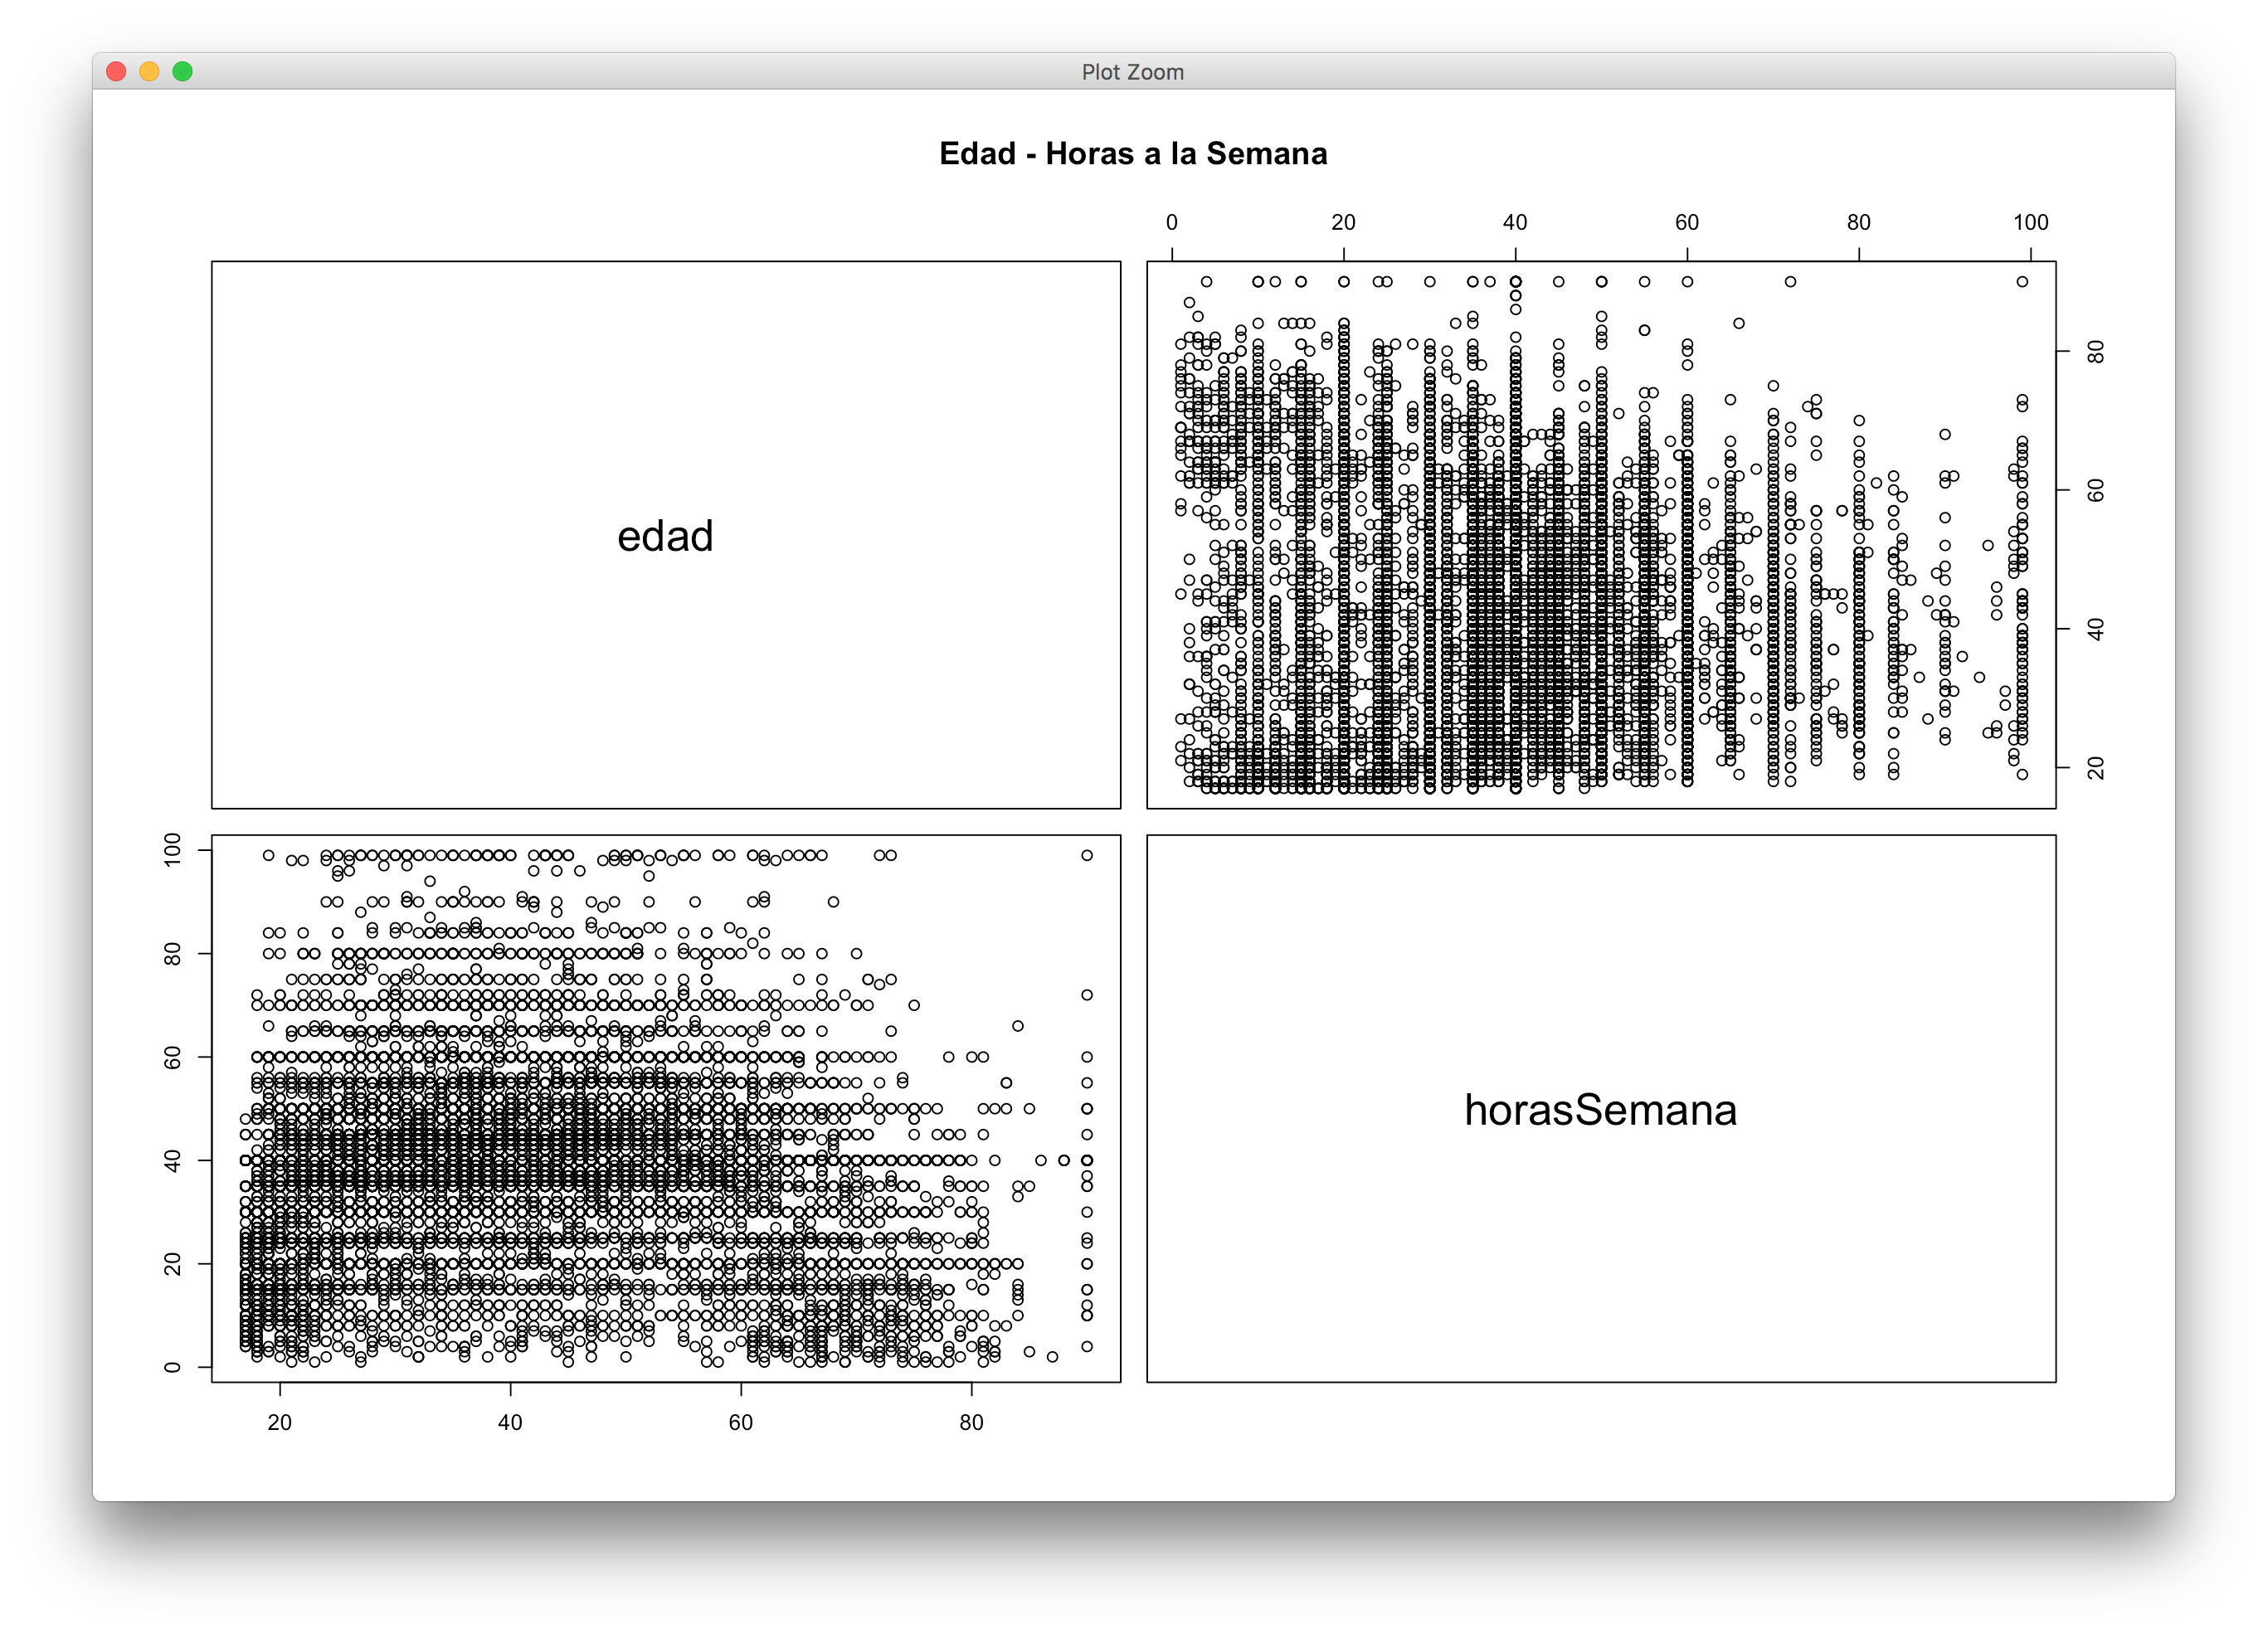
\includegraphics[scale=0.45]{graficas/edadHoras}}
  \end{center}
  \begin{center}
    \hbox{\hspace{-5.5em}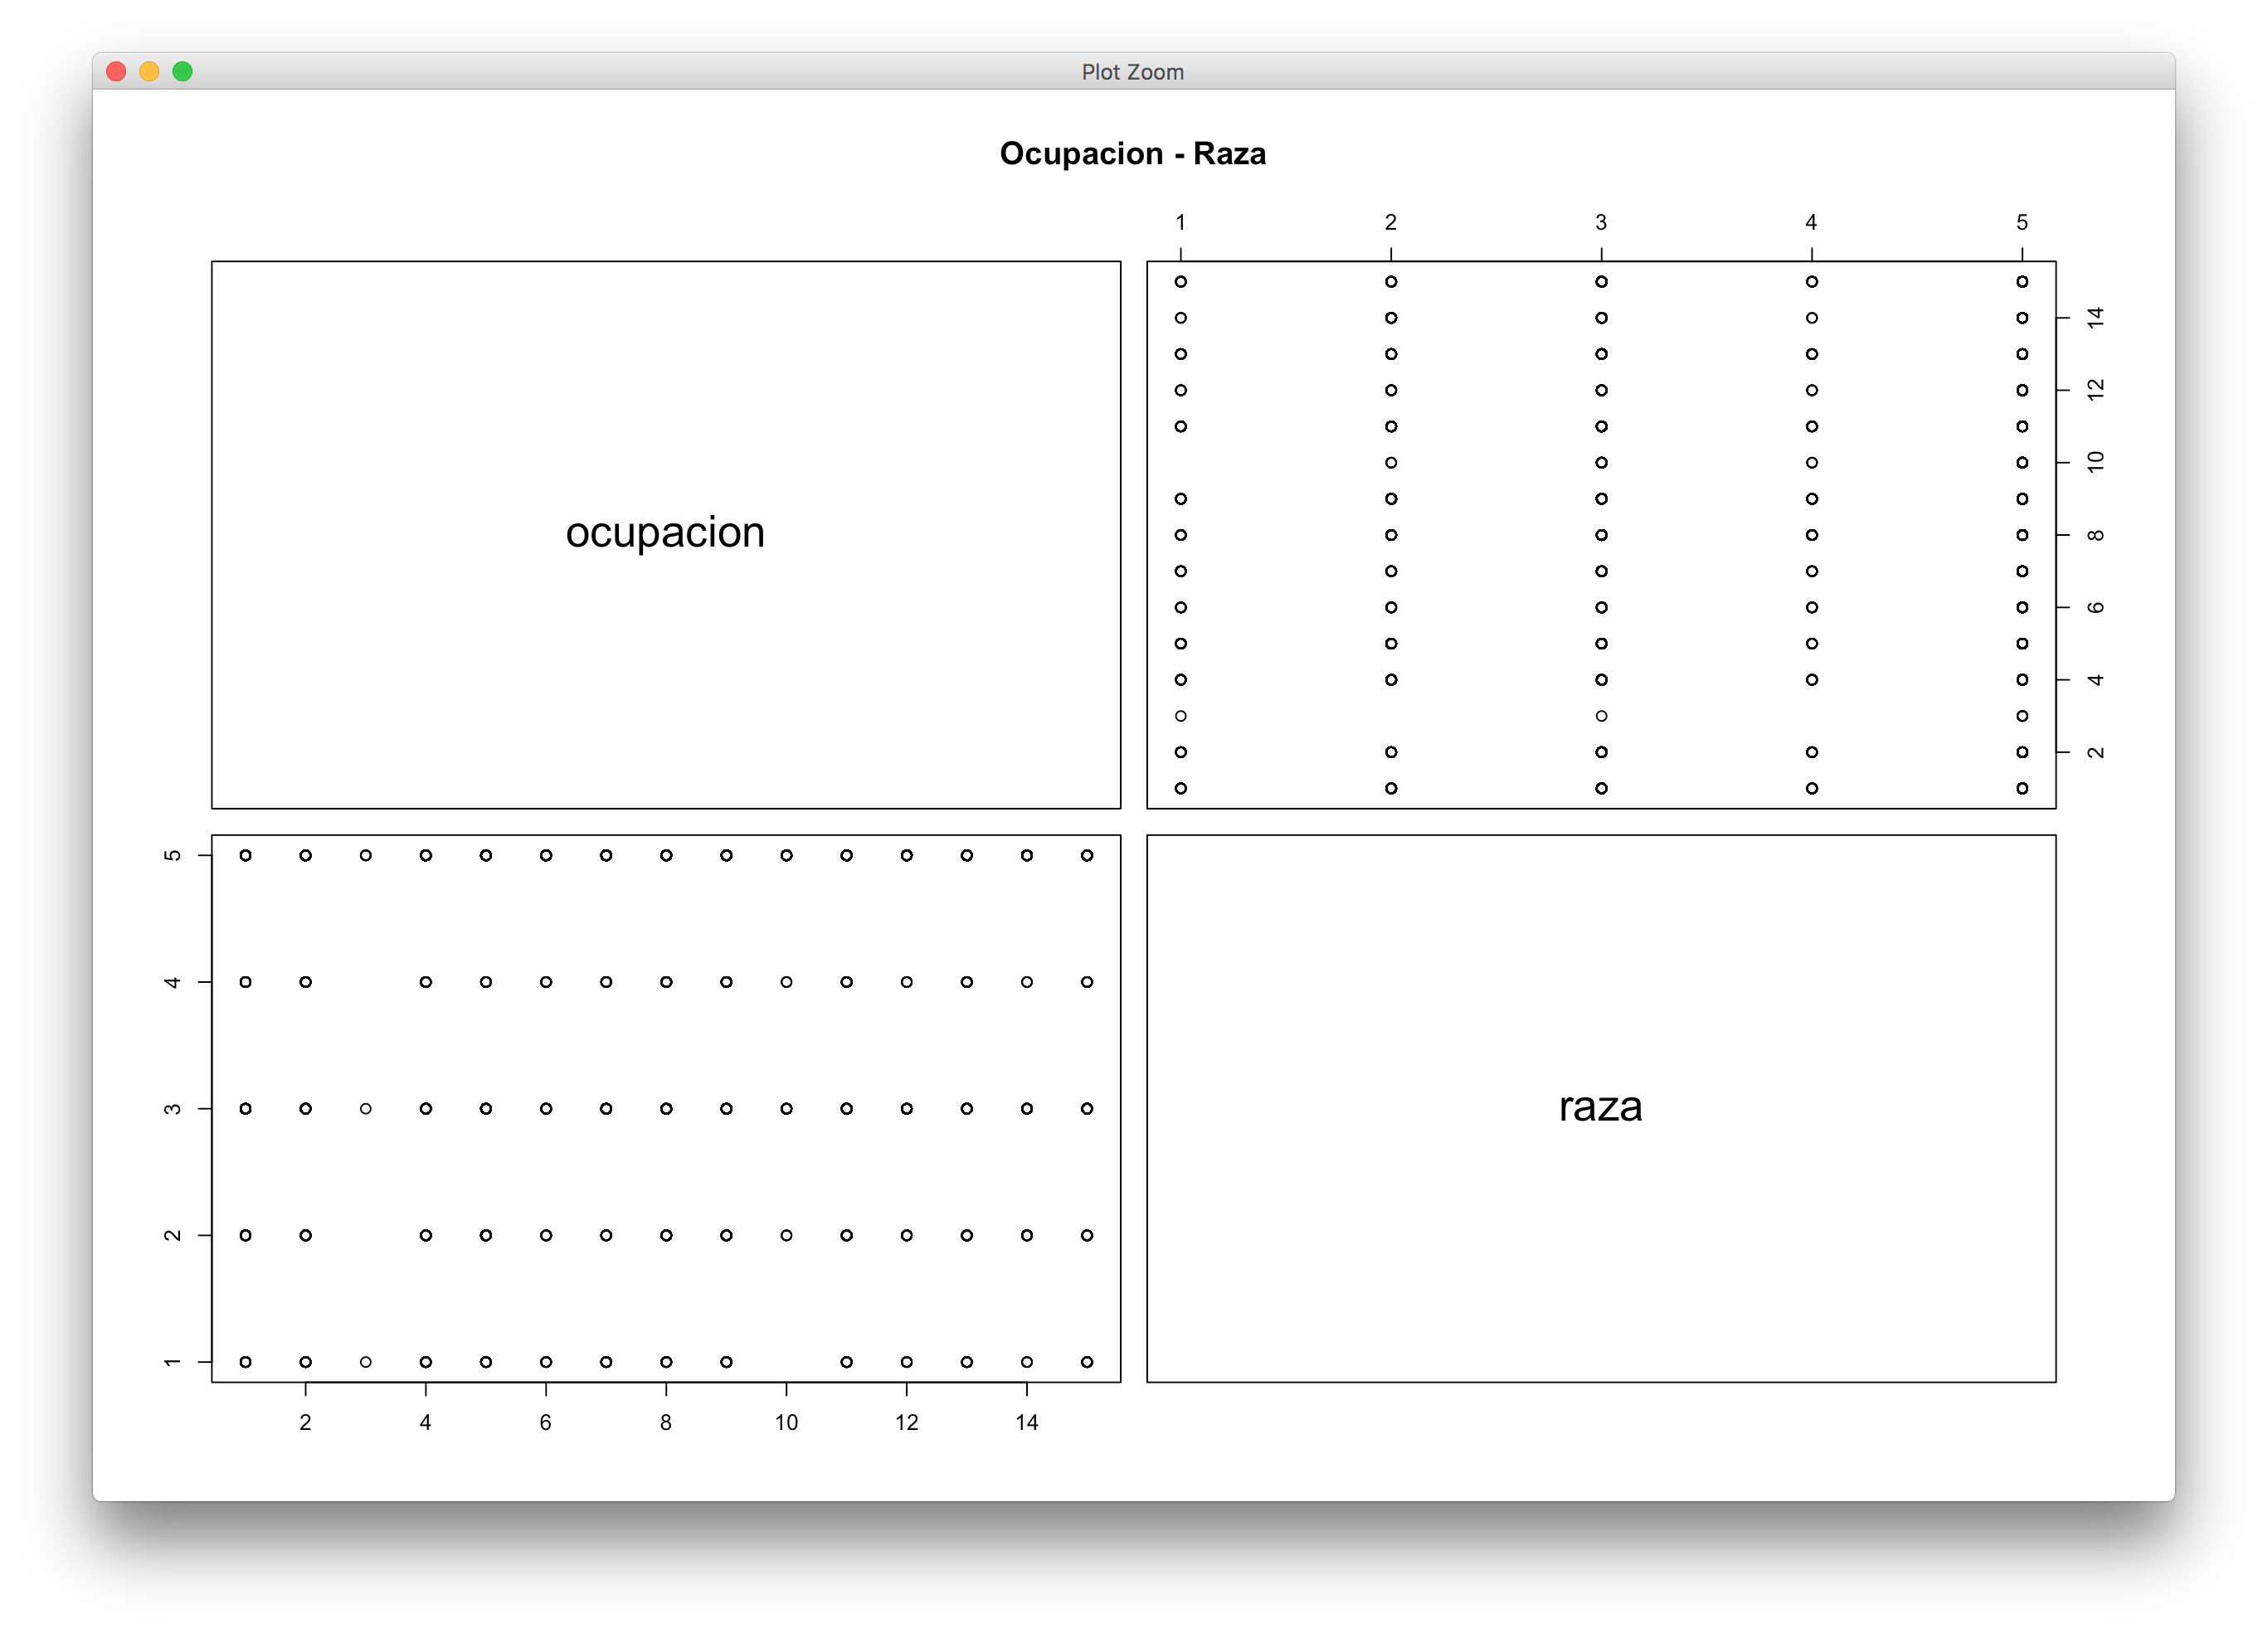
\includegraphics[scale=0.45]{graficas/ocupacion-raza}}
  \end{center}
  \begin{center}
    \hbox{\hspace{-5.5em}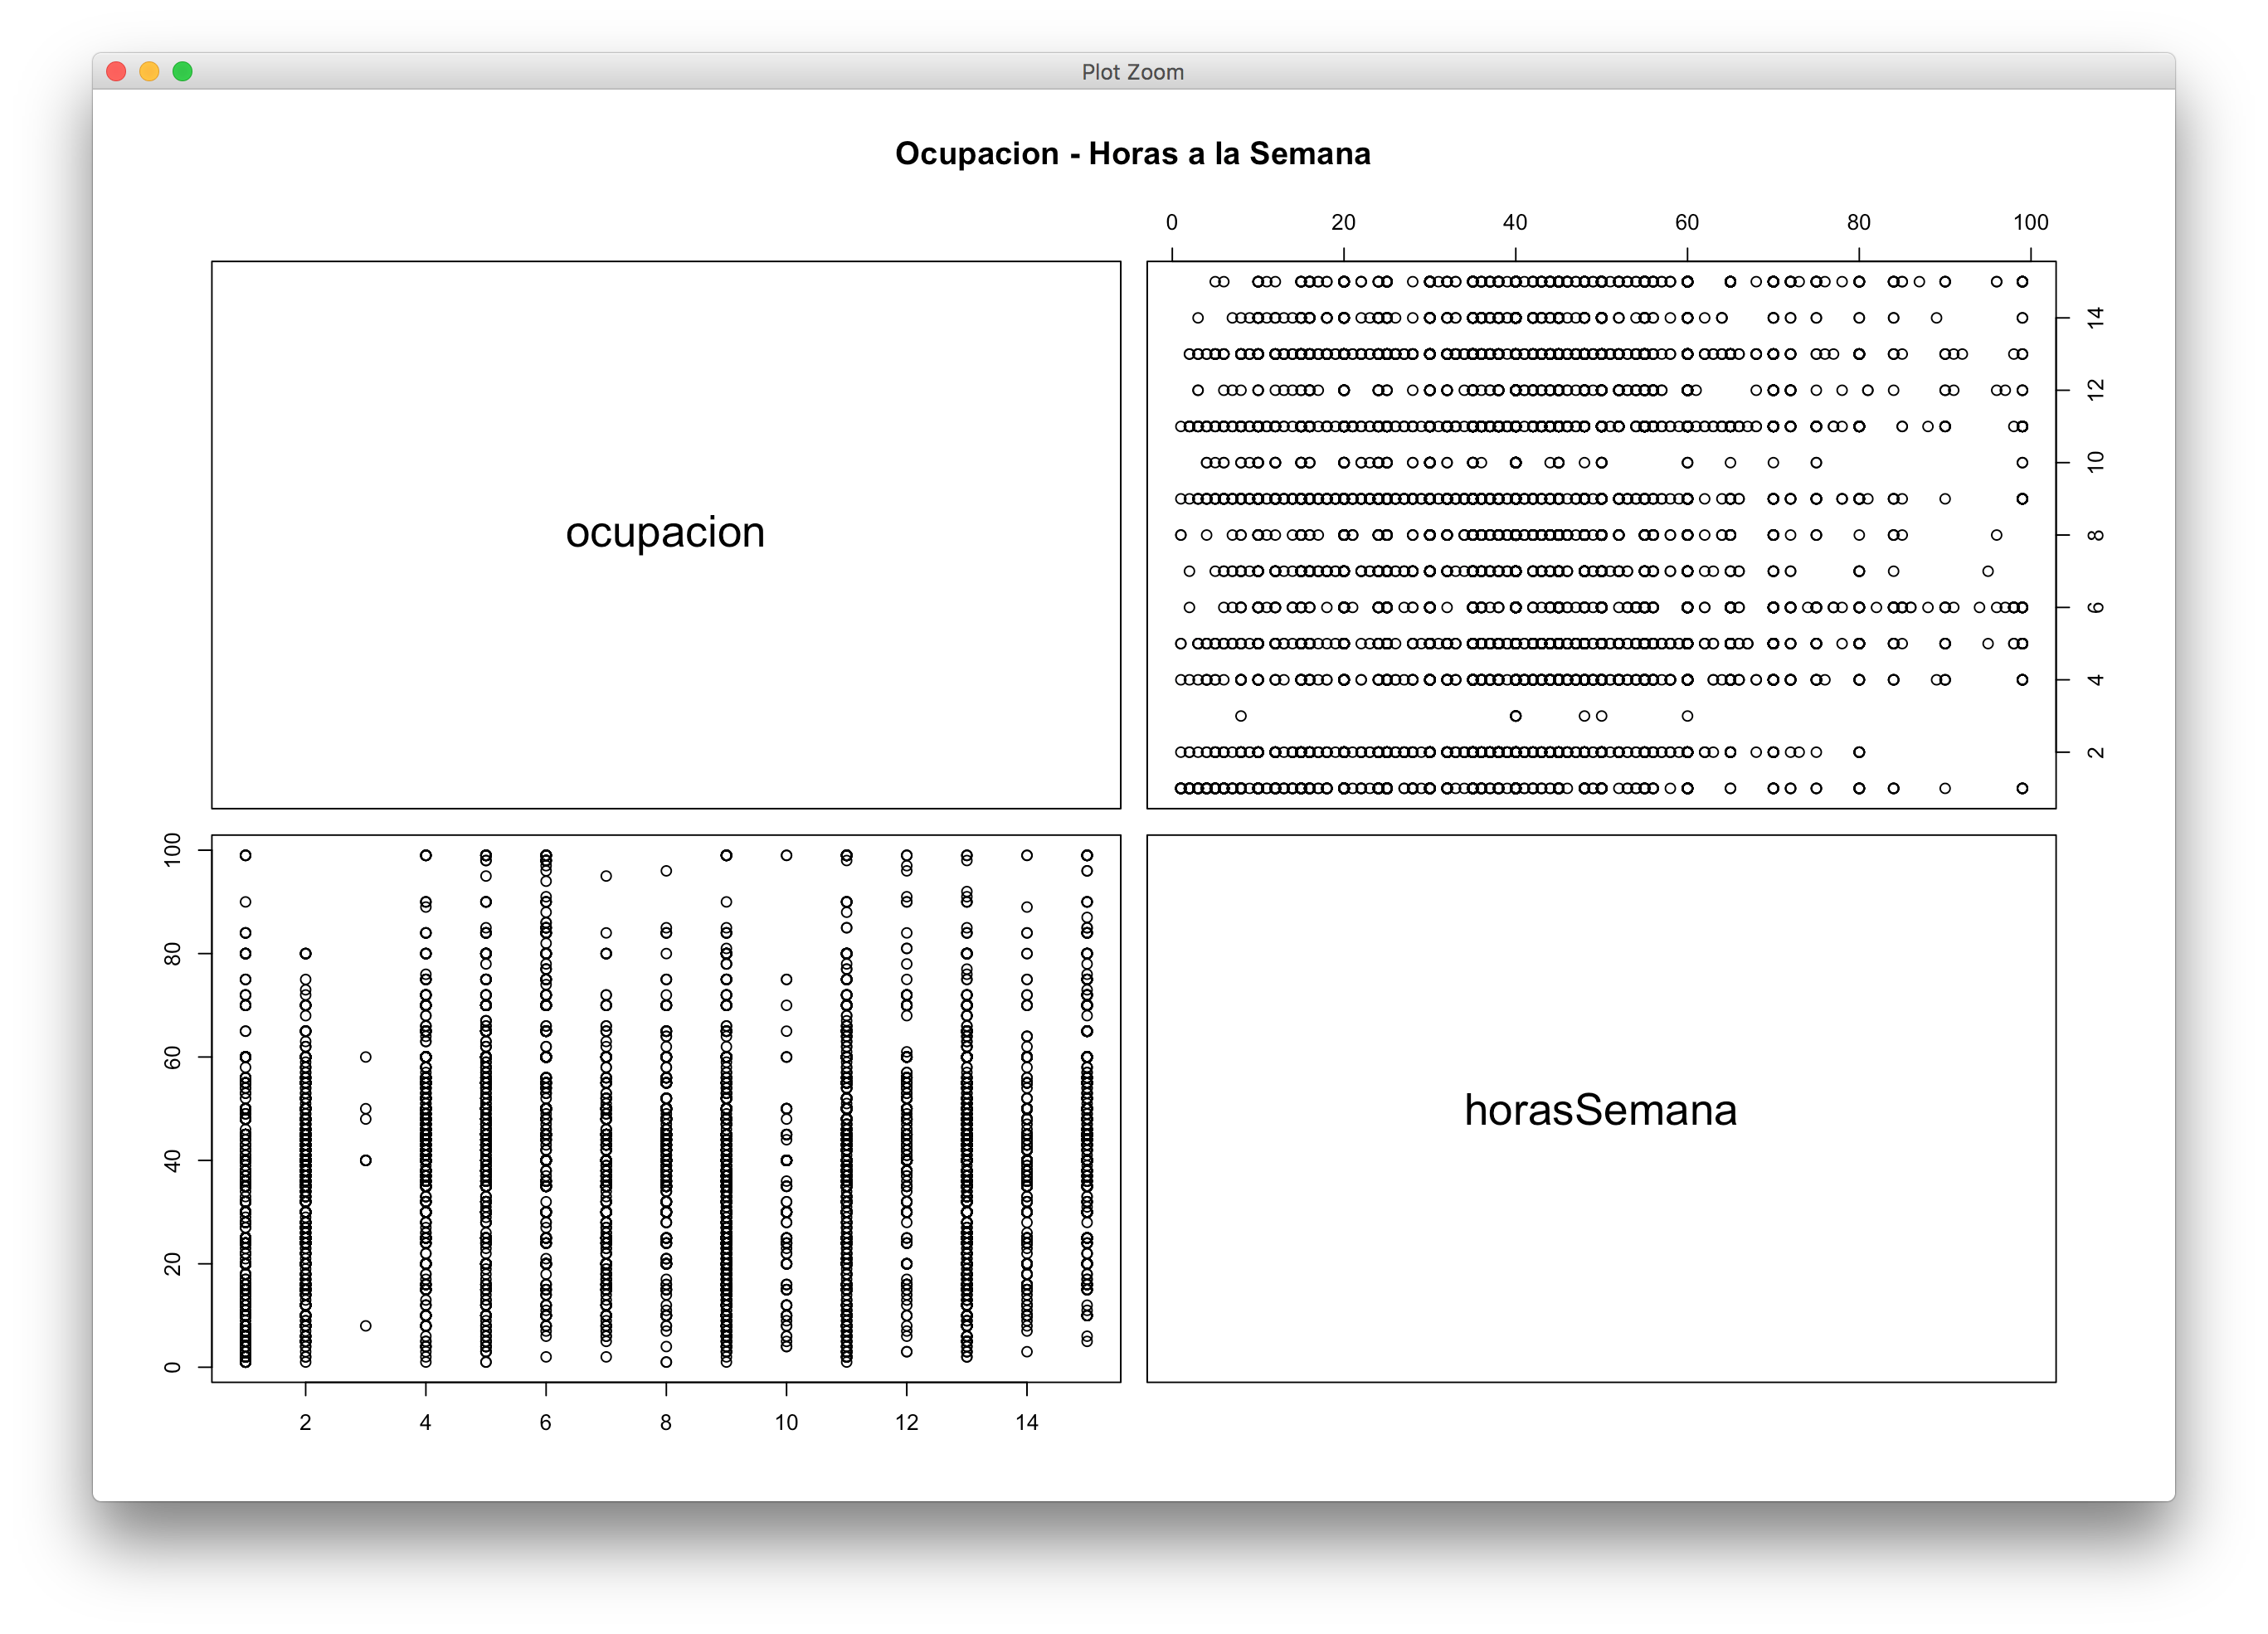
\includegraphics[scale=0.45]{graficas/ocupacionHoras}}
  \end{center}
  \begin{center}
    \hbox{\hspace{-5.5em}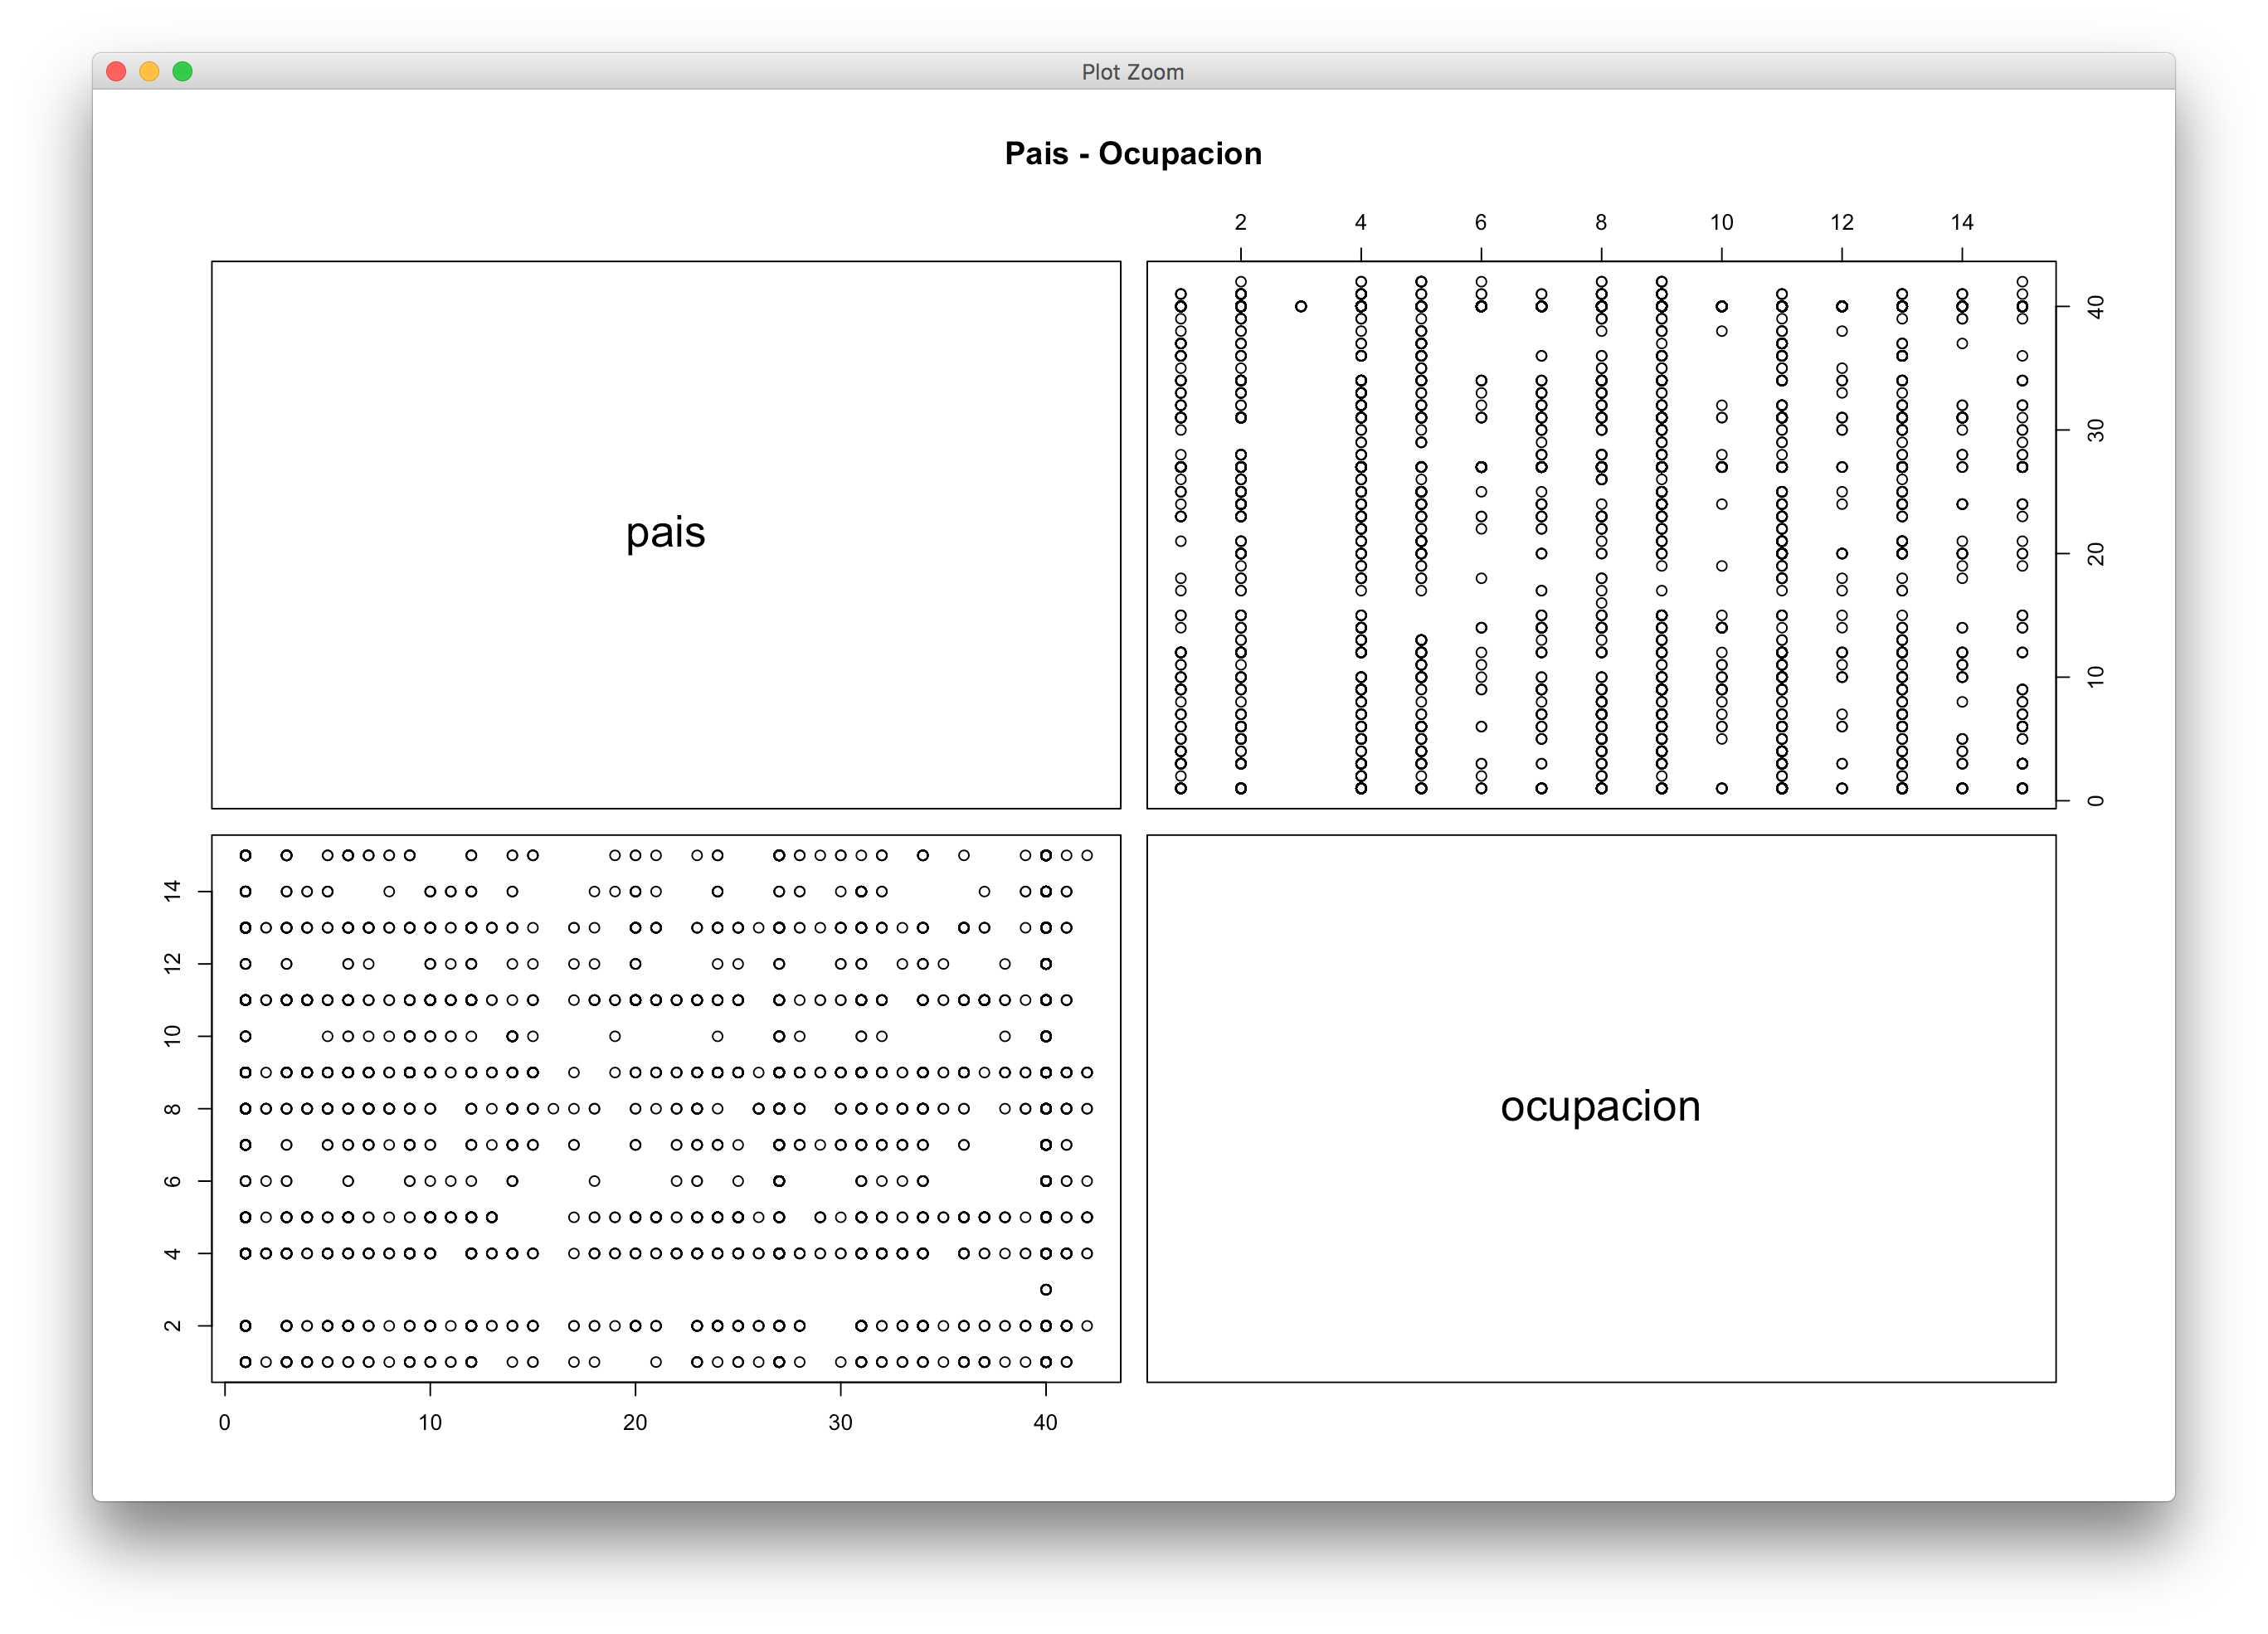
\includegraphics[scale=0.45]{graficas/pais-ocupacion}}
  \end{center}
  \begin{center}
    \hbox{\hspace{-5.5em}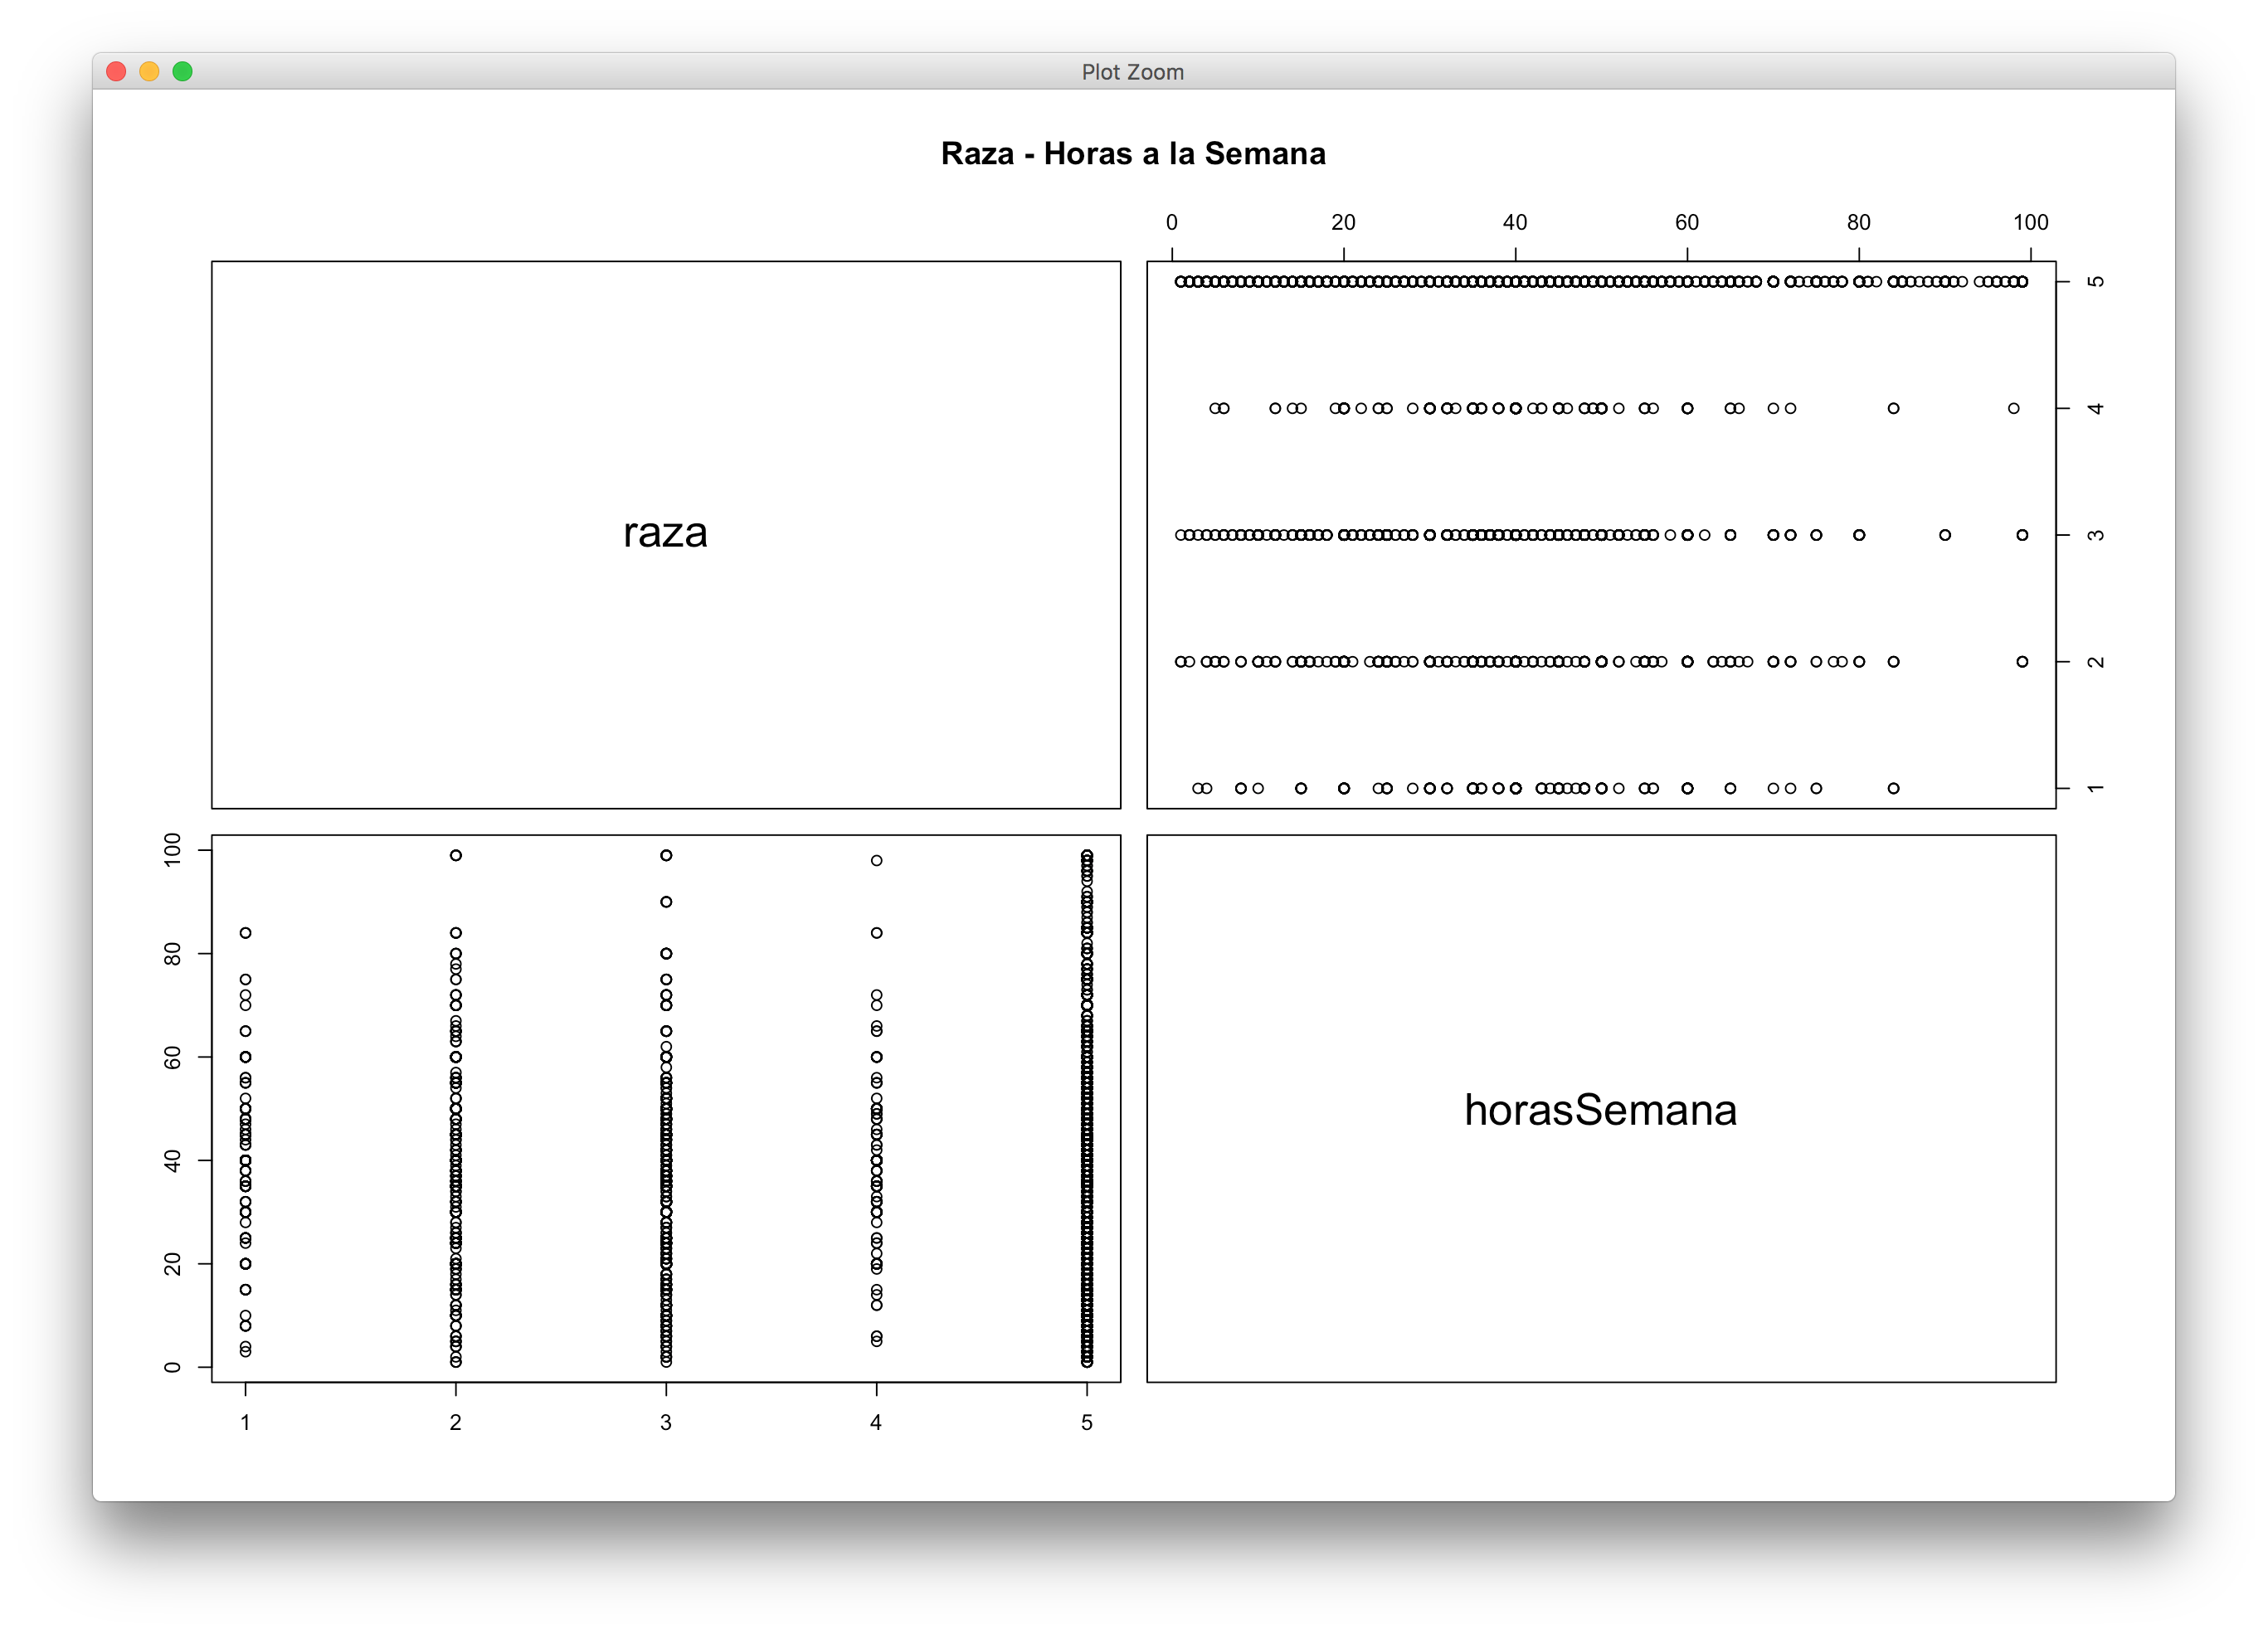
\includegraphics[scale=0.45]{graficas/raza-horas}}
  \end{center}
  \begin{center}
    \hbox{\hspace{-5.5em}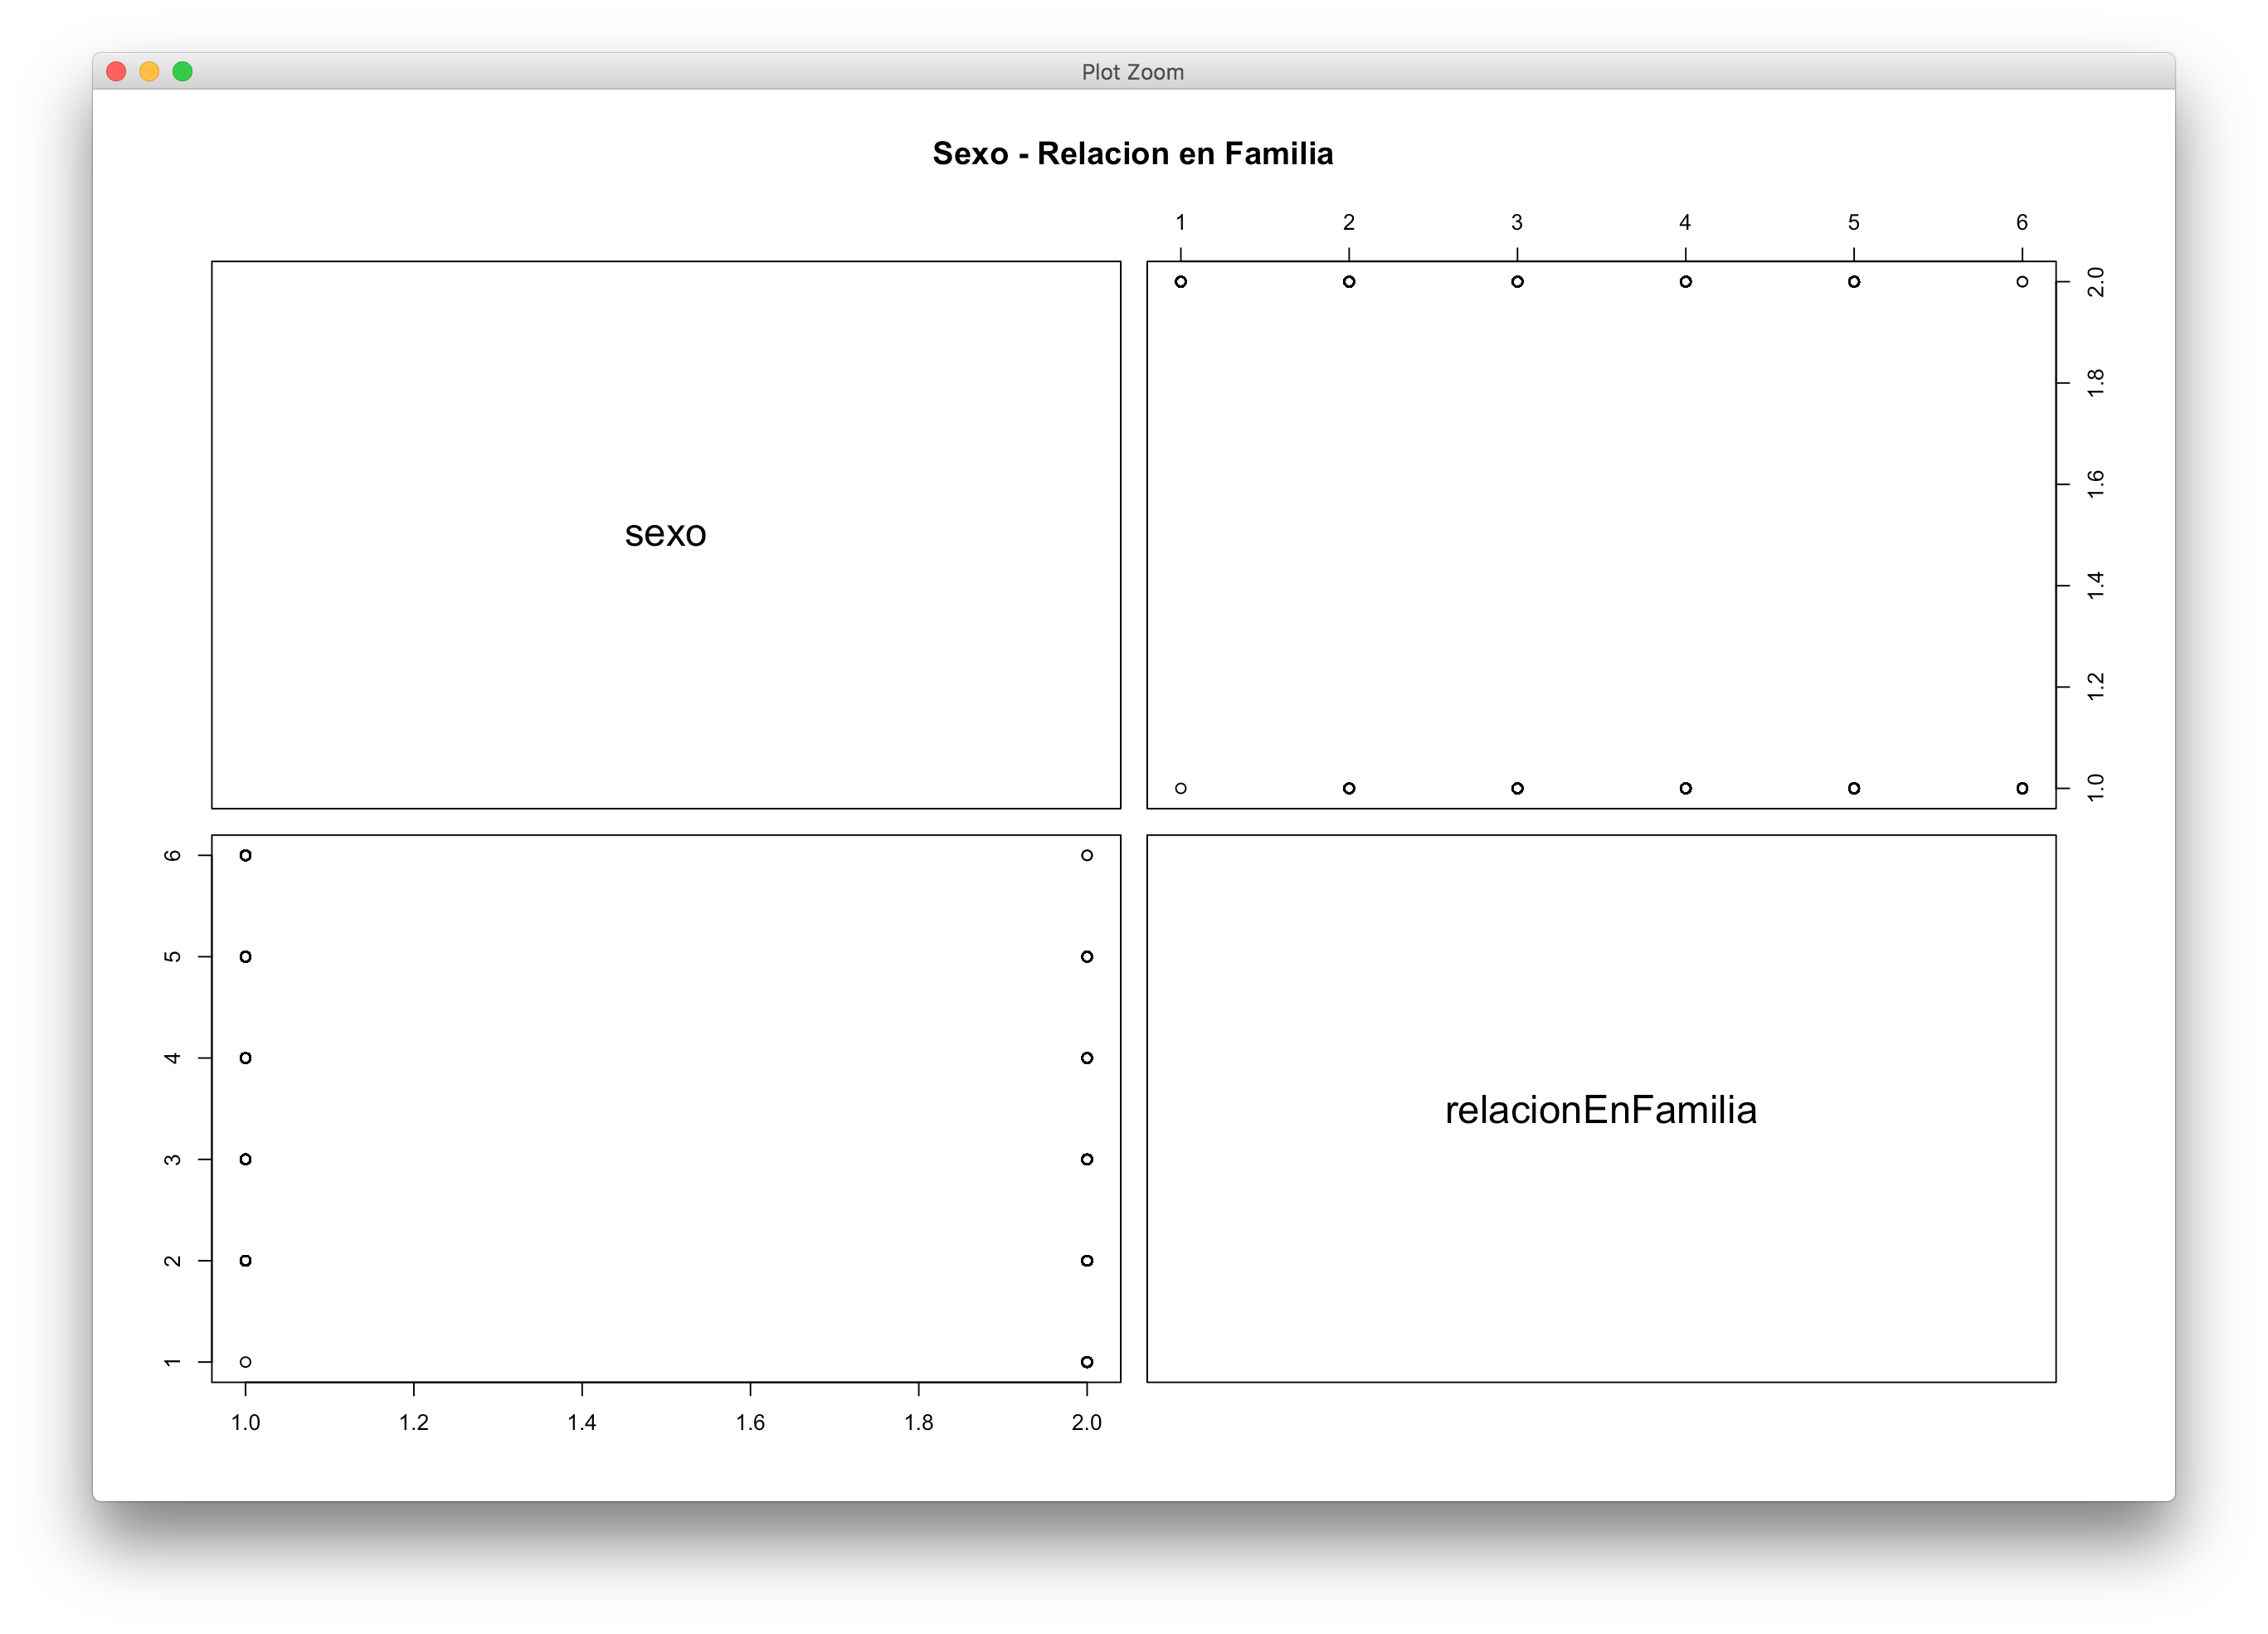
\includegraphics[scale=0.45]{graficas/Sexo-RelFam}}
  \end{center}
\section{Preprocesamiento}
Podemos observar que {\it education} es lo mismo que {\it education\_num}, es decir, si el grado en {\it education} es 'Doctorate' entonces {\it education\_num} será 16, si es 'Masters' será 14, y asi sucesivamente. Por lo que nos deshicimos deshacer de {\it education\_num}, también nos deshicimos de {\it fnlwgt} ya que nos proporciona información de grupos con caracteristicas demográficas parecidas, pero no sabemos el significado exacto del número, porque en la documentación del conjunto de datos no viene como es obtenido, para los datos que son numericos como {\it age} y {\it hours\_per\_week} los dividimos en rangos de 10\% y 5\% respectivamente. Para el atributo {\it native\_country} vimos que el que se repetia por mucho era 'United States', por lo que los dividimos en dos: 'United States' y 'Foreigner'. Hicimos algo parecido para {\it capital gain} y {\it capital loss} los dividimos por cero y mayor a cero. Vistos en tablas de frecuencias nos quedaron de la siguiente manera: estas se pueden encontrar en el archivo {\it preprocesamiento.sql}
  \begin{center}
    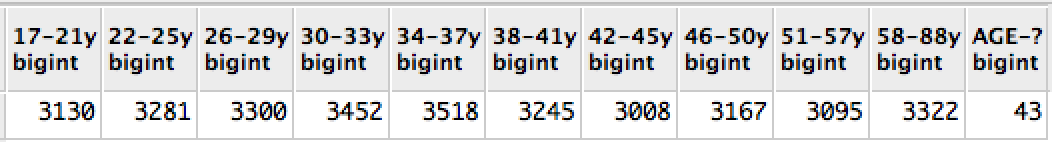
\includegraphics{tablas/age}
  \end{center}
  En esta tabla podemos observar que el rango mas alto es de 21 a 40 años mientras que el menor es de 81 a 100 años, también el otro que se repute bastante son las edades que están en tres 41 y 60 años, entonces podríamos decir que en general las personas de nuestro conjunto de datos se encuentran en el rango de 21 a 60 años.
  \begin{center}
    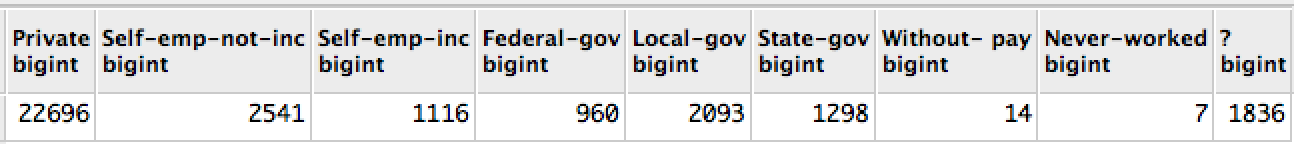
\includegraphics[scale=0.5]{tablas/workclass}
  \end{center}
  La mayoría de la gente de nuestro conjunto de datos tiene un trabajo en el sector privado, este tiene una gran diferencia con respecto a los demás, las demás clases de trabajo no rebasan las 4,000 repeticiones, lo cual es demasiado pequeño.
  \begin{center}
    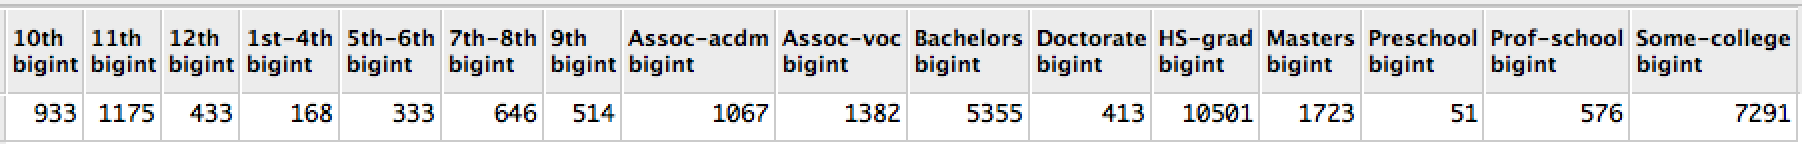
\includegraphics[scale=0.5]{tablas/education}
  \end{center}
  La mayoría de la gente tiene un máximo grado de educación de  preparatoria, el que queda en segundo lugar es grado universitario. Podemos observar que los menores son los que tienen menor grado de estudios van de preescolar a sexto grado. También muy pocos tienen el grado de doctor.
  \begin{center}
    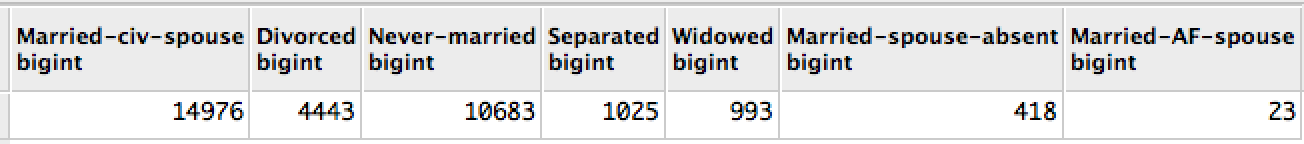
\includegraphics[scale=0.5]{tablas/maritalstatus}
  \end{center}
  Mas de la mitad de las personas están casados, mientras que una tercera parte nunca se ha casado. Los estados civiles mas repetidos quedan ordenados de forma descendente de la siguiente manera: casado, nunca casado y divorciado.
  \begin{center}
    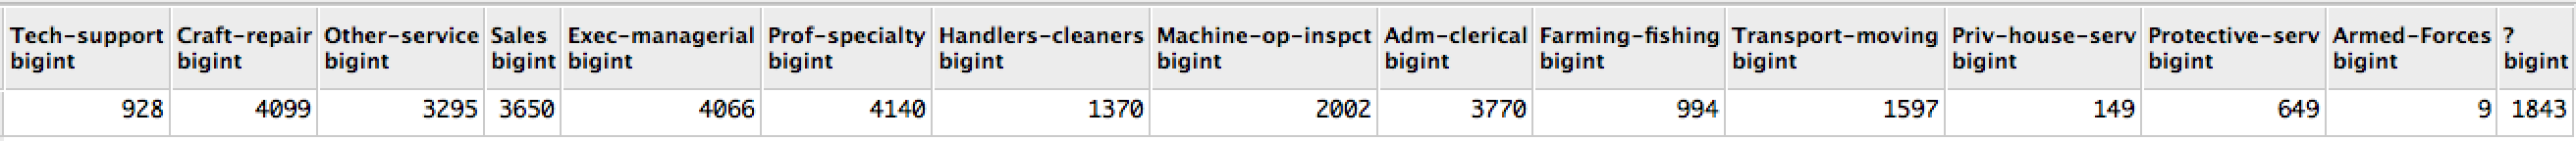
\includegraphics[scale=0.5]{tablas/occupation}
  \end{center}
  Podemos observar que 6 ocupaciones por lo menos se repiten mas de 3,000 veces, mientras que 9 ocupaciones están por debajo de 2,000. Es importante resaltar que no sabemos la ocupación de 2,000 personas.
  \begin{center}
    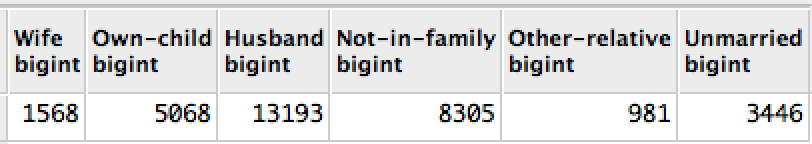
\includegraphics{tablas/relationship}
  \end{center}
  Mezclando la gráfica de sexo y relación en familia podemos observar que casi la mitad de los hombres juegan el papel de Esposo, mientras que solo una pequeña parte de las mujeres tiene el papel de esposa.
  \begin{center}
    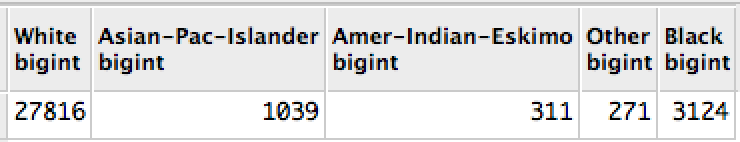
\includegraphics{tablas/race}
  \end{center}
  Mas del 70\% de las personas de nuestro conjunto de datos es de raza Blanca.
  \begin{center}
    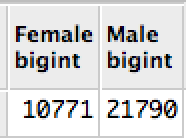
\includegraphics{tablas/sex}
  \end{center}
  Mas del 60\% de nuestra población es hombre.
  \begin{center}
    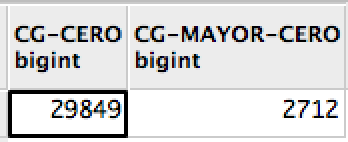
\includegraphics{tablas/capitalgain}
  \end{center}
  Podemos observar que mas de la mitad tiene 0
  \begin{center}
    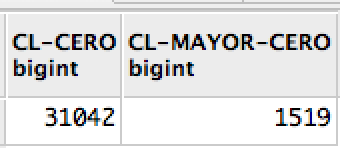
\includegraphics{tablas/capitalloss}
  \end{center}
  Lo mimso que en el anterior la mayoria tiene valor cero.
  \begin{center}
    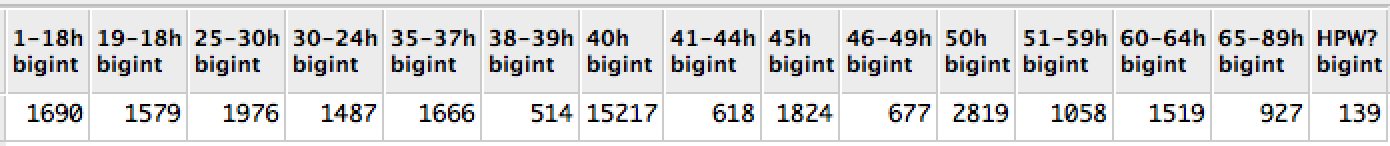
\includegraphics[scale=0.5]{tablas/hpw}
  \end{center}
  La mayoría de las personas trabajan entre 21 a 40 horas a la semana.
  \begin{center}
    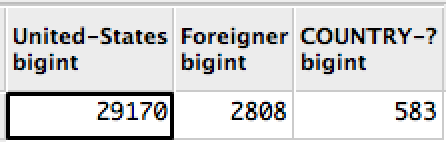
\includegraphics{tablas/nativecountry}
  \end{center}
  El país que predomina bastante es estados unidos.
  \begin{center}
    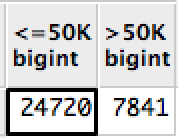
\includegraphics{tablas/total}
  \end{center}
  En total mas de la mitad de la gente gana menos de 50k.

\end{document}
